\chapter{Event selection and reconstruction}

In this chapter the procedure for reconstruction of the events where one $B$ meson decays inclusively
to a $\Lambda_c$ baryon and the accompanying $B$ meson decays hadronically is illustrated.

\section{$B_{tag}$ reconstruction}

The FEI is an exclusive tagging algorithm that uses machine learning to reconstruct
$B$ meson decay chains and calculates the probability that these decay chains correctly
describe the true process. In this analysis only hadronically reconstructed decay chains are
considered. The training called \texttt{FEI\_}\texttt{B2BII\_}\texttt{light-2012-minos} is used. Tag-side $B$ meson candidates are required to have a beam-constrained mass greater than 5.22 GeV/c$^2$ and $- 0.15 < \Delta E < 0.07 $   GeV. \\
In the case of multiple candidates in the same event, the candidate with the highest SignalProbability (the signal probability calculated by FEI using FastBDT) is chosen. To suppress the background constisting of $B^0$ events misreconstructed as $B^+$ (and vice-versa) from neutral (charged) decays also a $B^0$ ($B^+$) candidate is reconstructed with FEI and if its SignalProbability is higher than the charged (neutral) reconstructed $B$ meson, the event is discarded. This constitutes a sort of crossfeed-veto, rejecting part of events belonging to the other typology of decays of interest: for example in the case one is interested in reconstructing $B^{+/-}$ decays and the event actually contains $B^0/\bar{B^0}$ decays, the FEI reconstructed neutral $B$ meson candidate most likely presents a higher SignalProbability than the charged FEI reconstructed candidate.

\section{$\Lambda_c$ reconstruction}

In the \textit{rest of event} (ROE) of the reconstructed $B_{tag}$ meson, to select $\Lambda_c \rightarrow p  K \pi$ signal candidates, the following event selection criteria are applied (same PID cuts were used for example in the Belle Note 1521 \url{https://belle.kek.jp/secured/belle_note/gn1521/BN_v1.pdf}). 
Charged tracks with the impact parameters perpendicular to and along the nominal interaction point (IP) are required to be less than 2 cm and 4 cm respectively ($dr <$ 2 cm and $|dz| <$ 4 cm).\\
The pion tracks are required to be identified with $\frac{\mathcal{L_{\pi}}}{\mathcal{L}_{K}+\mathcal{L_{\pi}}} > 0.6$. The kaon tracks are required to be identified with $\frac{\mathcal{L}_{K}}{\mathcal{L_{K}}+\mathcal{L_{\pi}}} > 0.6$, and the proton/anti-proton tracks are required to be identified with  
$\frac{\mathcal{L}_{p/\bar{p}}}{\mathcal{L}_{K}+\mathcal{L}_{p/\bar{p}}} > 0.6$ and $\frac{\mathcal{L}_{p/\bar{p}}}{\mathcal{L}_{\pi}+\mathcal{L}_{p/\bar{p}}} > 0.6$, where the $\mathcal{L}_{\pi ,} {}_{K,} {}_{p/\bar{p}}$ are the likelihoods for pion, kaon, proton/anti-proton, respectively, determined using the ratio of the energy deposit in the ECL to the momentum measured in the SVD and CDC, the shower shape in the ECL, the matching between the position of charged
track trajectory and the cluster position in the ECL, the hit information from the
ACC and the dE/dx information in the CDC. \\
For the $\Lambda_c$ candidates a vertex fit is performed with \texttt{TreeFitter}, requiring it to converge.  If there are more than one $\Lambda_c$ combination, then the best candidate based on the $\chi^2$ probability is chosen. The $\Lambda_c$ signal region is defined to be $|M_{\Lambda_c} - m_{\Lambda_c}| < $   20  MeV/$c^2$ ($\sim$ 3$\sigma$), here $m_{\Lambda_c}$ is the nominal mass of $m_{\Lambda_c}$.\\



\begin{figure}[H]
%\centering
{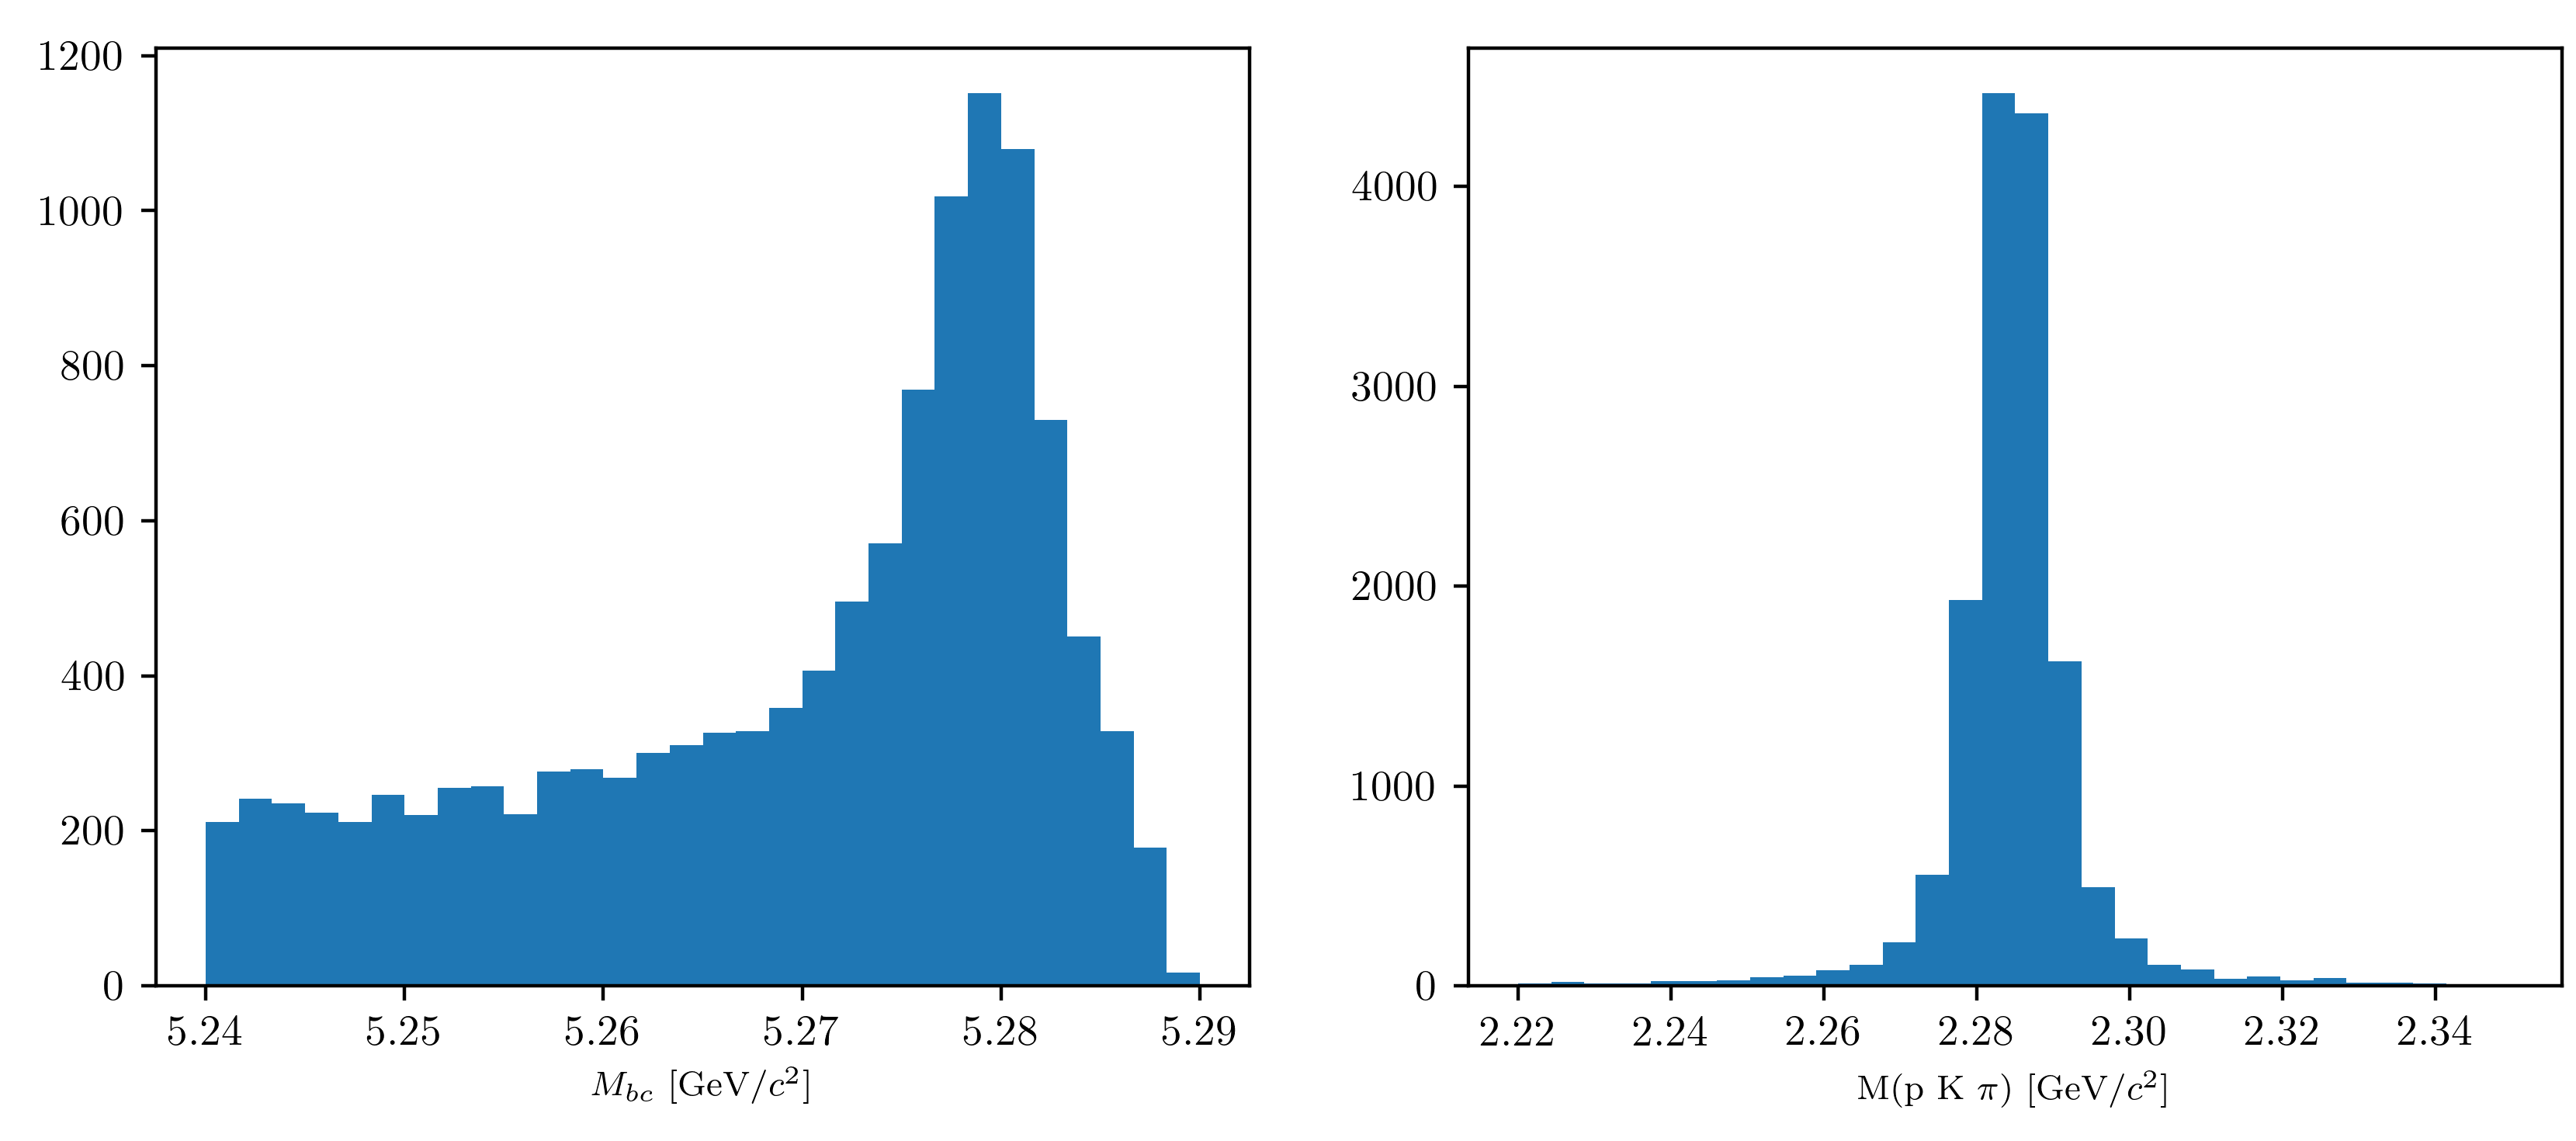
\includegraphics[width=1.0\textwidth]{03-Selection/figs/chargedBcorr_Mbc_MpKpi_TotalSignal.png}}
\caption{$M_{bc}$ and $M(p K \pi)$ distributions of $B_{tag}$ and $\Lambda_c$ candidates reconstructed in the signal sample.}
\label{fig:chargedBcorr_Mbc_MpKpi_TotalSignal}
\end{figure}

\section{Wrongly reconstructed $B_{tag}$ candidates}\label{wronglyBtag}

In the case of the signal sample the distributions for the beam-constrained mass $M_{bc}$ and for the correctly reconstructed $\Lambda_c$ candidates, look
like in \cref{fig:chargedBcorr_Mbc_MpKpi_TotalSignal}. If one then investigates the $M_{bc}$ distribution of the $B_{tag}$ candidates reconstructed with 
FEI, it can be seen that there is a peaking structure for wrongly reconstructed $B$ 
mesons (as in \cref{fig:wrongly_recoB}), according to the BASF2 internal truth matching variable \textbf{isSignal}.
It is obvious from this that the BASF2 internal truth matching variable cannot be used to separate properly the signal events in correctly and wrongly reconstructed $B$ mesons. In the study  BELLE2-NOTE-TE-2021-026 \url{https://docs.belle2.org/record/2711/files/BELLE2-NOTE-TE-2021-026.pdf} a possible solution was found developing new variables that can be used for an improved truth matching for the FEI (those variables were added to a newer BASF2 release than the one used for this study). In the present study instead a more "traditional" approach was adopted: fitting the $M_{bc}$ distribution with a sum of PDFs that account for the flat (background) component and the peaking (signal) component. The first component represents the combinatorial background, i.e. $B$ mesons that were mis-reconstructed, and therefore those events are denoted from now on as    "\textbf{misreconstructed signal}".  
The peaking component represents the correctly reconstructed signal events in $M_{bc}$ and therefore denoted from now on as "\textbf{reconstructed signal}".  Only the second one is then considered for the signal yield, while the first is counted as a background.
To validate this method a control decay study was performed on the flavor correlated $B^+ \rightarrow \bar{D^0}$ channel. 


\begin{figure}[h!]
\centering
{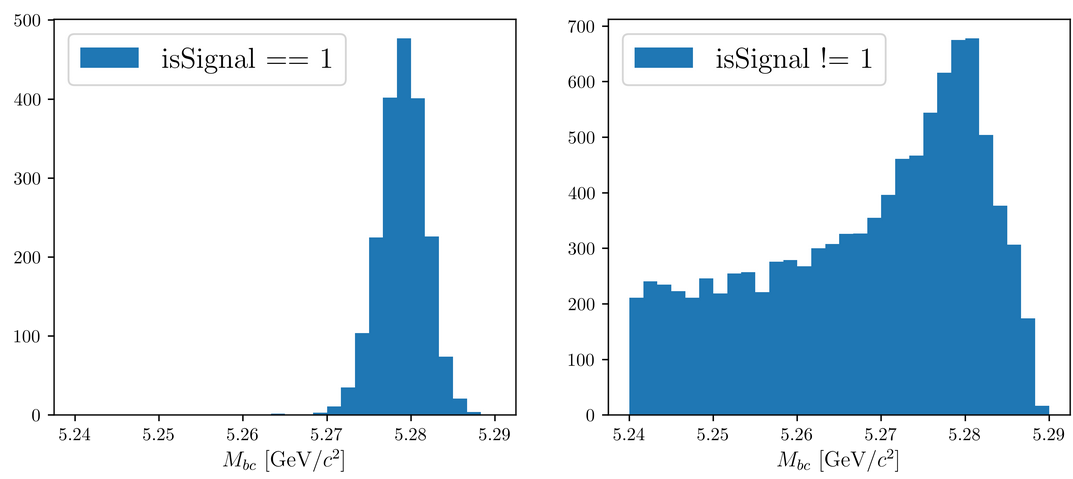
\includegraphics[width=1.\textwidth]{03-Selection/figs/wrongly_recoB.png}}
\caption{$M_{bc}$ distribution of $B_{tag}$ candidates reconstructed in the signal sample, truth-matched (on the left) and not (on the right).}
\label{fig:wrongly_recoB}
\end{figure}


\newpage

\section{Signal selection optimization}

To further enhance the purity of the signal decays, an optimization procedure is adopted to determine optimal cuts for a set of variables for each decay mode under investigation by this study.
The cuts on the following variables are optimized:
\begin{itemize}
    \item $foxWolframR2$: the event based ratio
of the 2-nd to the 0-th order Fox-Wolfram moments
    \item SignalProbability: the already mentioned signal probability calculated by FEI using FastBDT
    \item $p^{\Lambda_c}_{CMS}$: momentum of the $\Lambda_c$ candidates in the center of mass system
\end{itemize}

The optimization is based on the Figure Of Merit (FOM): FOM = $\frac{S}{\sqrt{S+B}}$

Where S and B are respectively signal and background events in the signal region: $M_{bc} > $ 5.27 GeV/$c^2$,  2.2665  $< M(p K \pi) <$ 2.3065 GeV/$c^2$.\\
Due to the issue reported in Sec. \ref{wronglyBtag}, to separate signal events that peak in $M_{bc}$ from the ones that are not (which are then categorized as background events), the events reconstructed in the signal sample are fitted. with a sum of Crystal Ball function and Argus for each cut value on the corresponding variable to optimize (as in \cref{fig:wrongB_Mbc}).

\begin{figure}[h!]
%\centering
{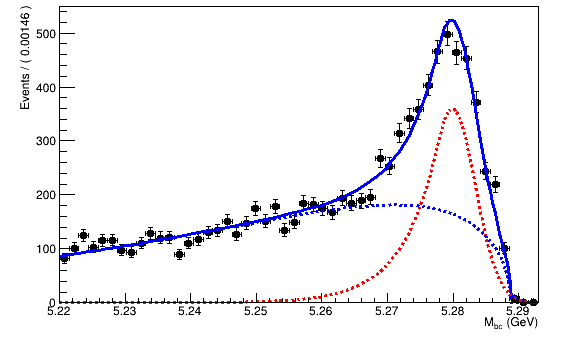
\includegraphics[width=0.75\textwidth]{03-Selection/figs/wrongB_Mbc.png}}
\caption{Example of a fit used to separate the correctly reconstructed $B$ mesons (described by the red dotted Crystal Ball function) from the wrongly reconstructed ones (described by the blue dotted Argus function).}
\label{fig:wrongB_Mbc}
\end{figure}

The next sections illustrate the procedure for each of the four decay channels.

\newpage

\subsection{$B^- \rightarrow \Lambda_c^+$ decays}
\label{sec:chargedCorrBtoLambdaC}

Here below the procedure of optimized signal selection of charged correlated decays is presented. 
\newline First, in order to suppress the continuum background the cut on $foxWolframR2$ is optimized. Fig. \ref{fig:R2distributions} shows the $foxWolframR2$ distributions for signal and continuum events. 
\begin{figure}[H]
%\centering
{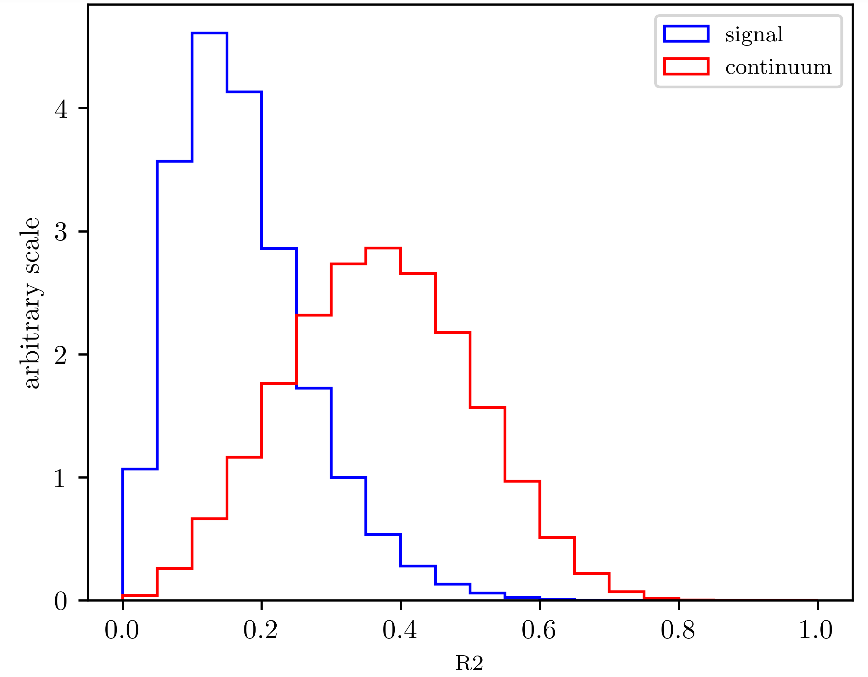
\includegraphics[width=0.75\textwidth]{03-Selection/figs/R2EventLevel_sig_qqbar_distributions.png}}
\caption{Distribution of the $foxWolframR2$ variable for signal and continuum background events.}
\label{fig:R2distributions}
\end{figure}


\begin{figure}[h!]
%\centering
{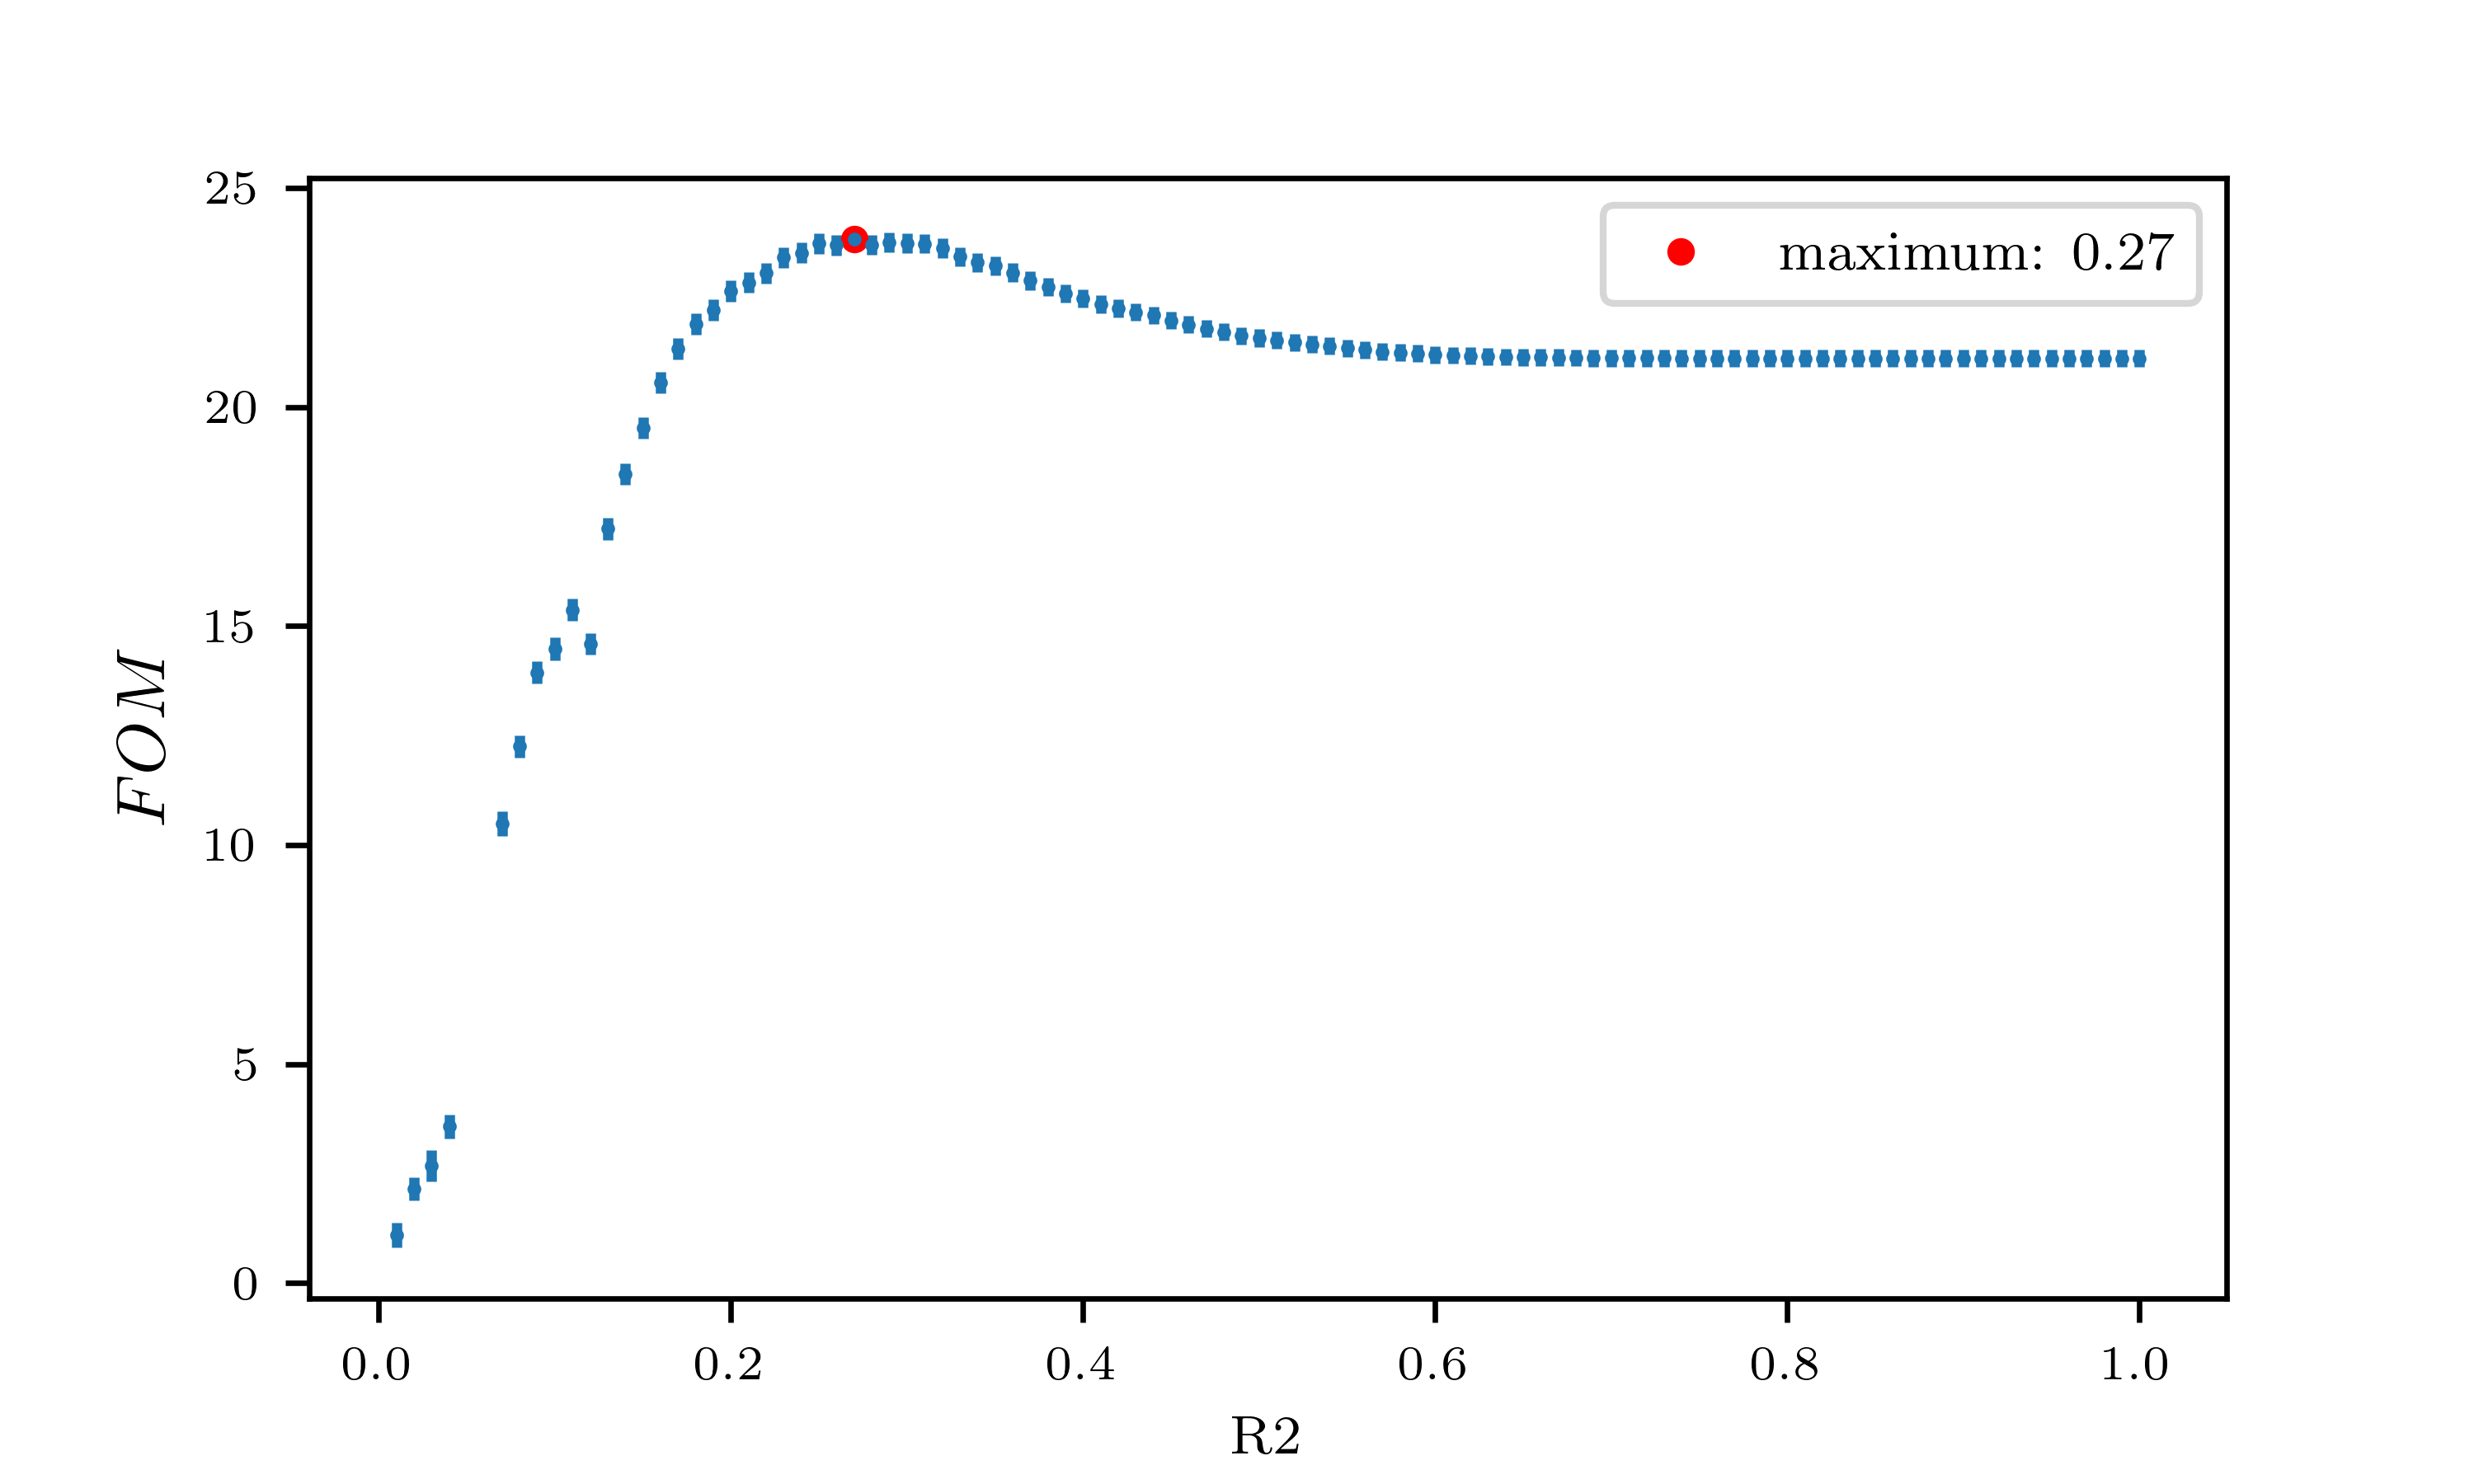
\includegraphics[width=0.65\textwidth]{03-Selection/figs/corr_chargedB_FOMvsR2_cut.png}}
\caption{Figure of Merit values calculated at several cuts on the $foxWolframR2$ variable}
\label{fig:corr_chargedB_FOMvsR2_cut}
\end{figure}

With the optimized cut $foxWolframR2 < 0.27$ (corresponding to the maximum of the FOM curve shown in Fig. \ref{fig:corr_chargedB_FOMvsR2_cut}), the cut on SignalProbability is optimized in the same way (see Fig. \ref{fig:corr_chargedB_FOMvsSigProb_cut}).


\begin{figure}[H]
%\centering
{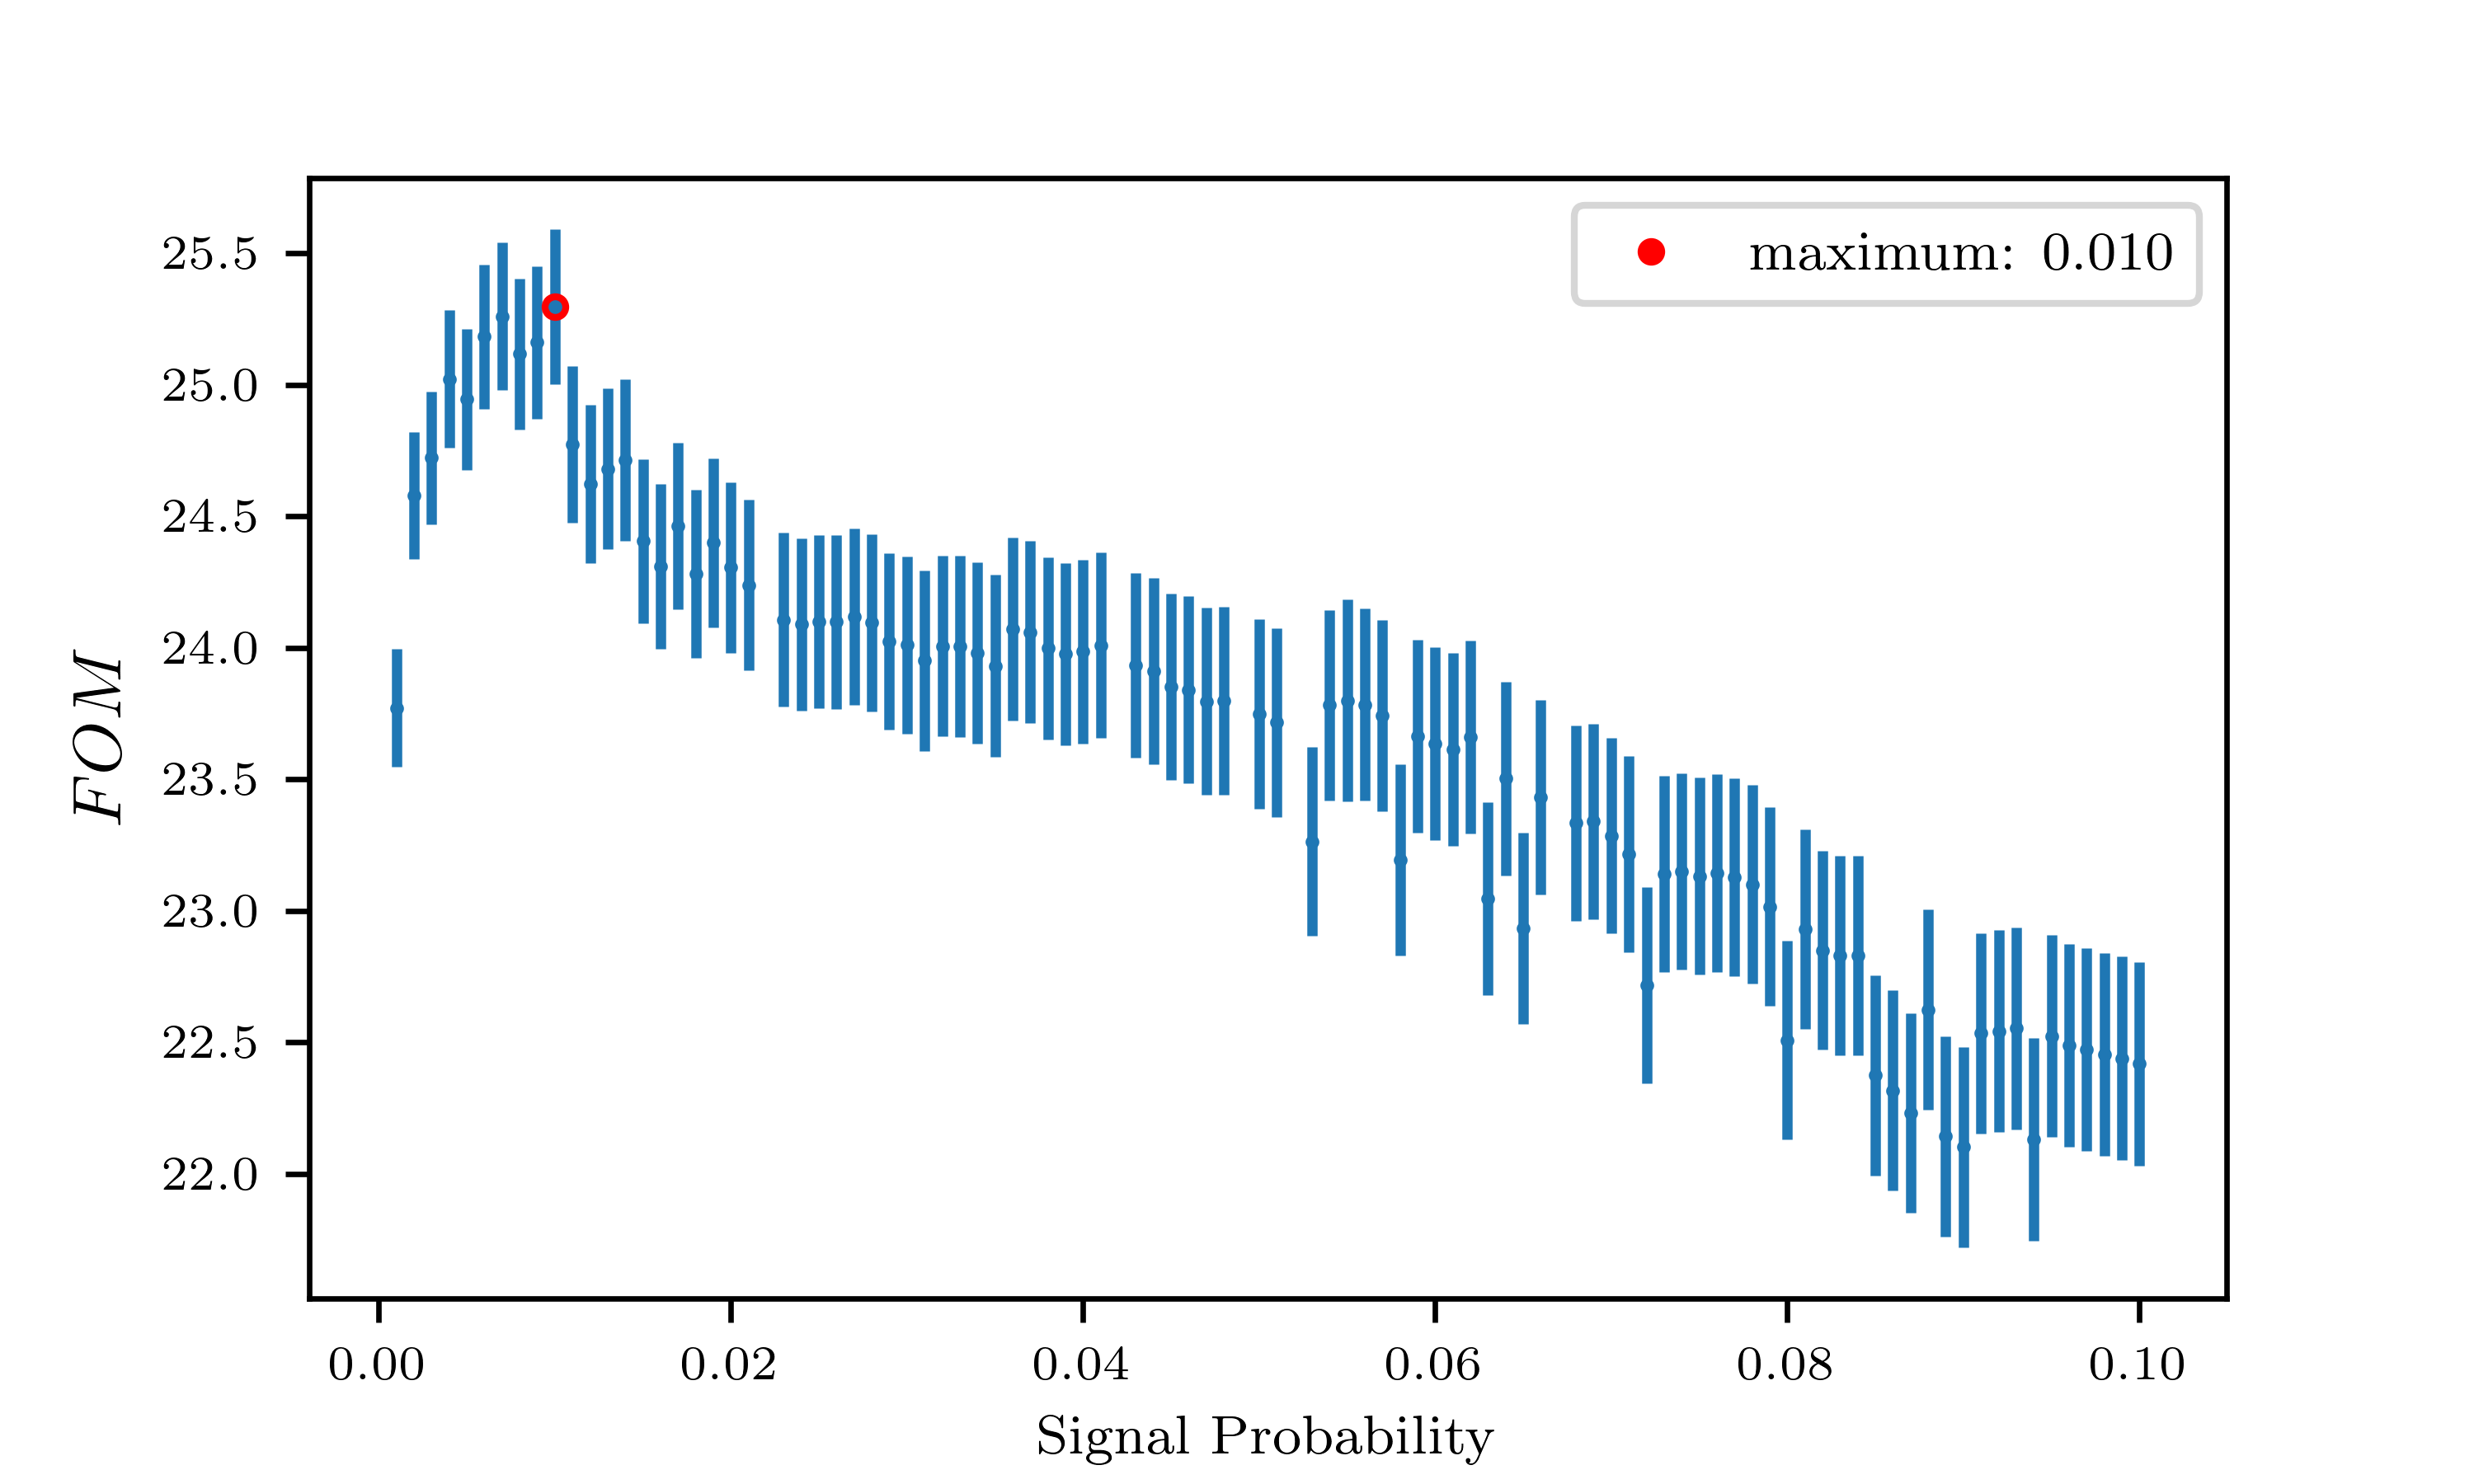
\includegraphics[width=0.75\textwidth]{03-Selection/figs/corr_chargedB_FOMvsSigProb_cut.png}}
\caption{Figure of Merit values calculated at several cuts on the SignalProbability variable}
\label{fig:corr_chargedB_FOMvsSigProb_cut}
\end{figure}

With the optimized cut SignalProbability $ > $ 0.01, the cut on $foxWolframR2$ variable is rechecked (Fig. \ref{fig:corr_chargedB_FOMvsR2_cut_SigProbOpt}). Being the maximum values fluctuating around $foxWolframR2 < 0.3$, this cut is the one finally chosen for this variable.   

\begin{figure}[H]
%\centering
{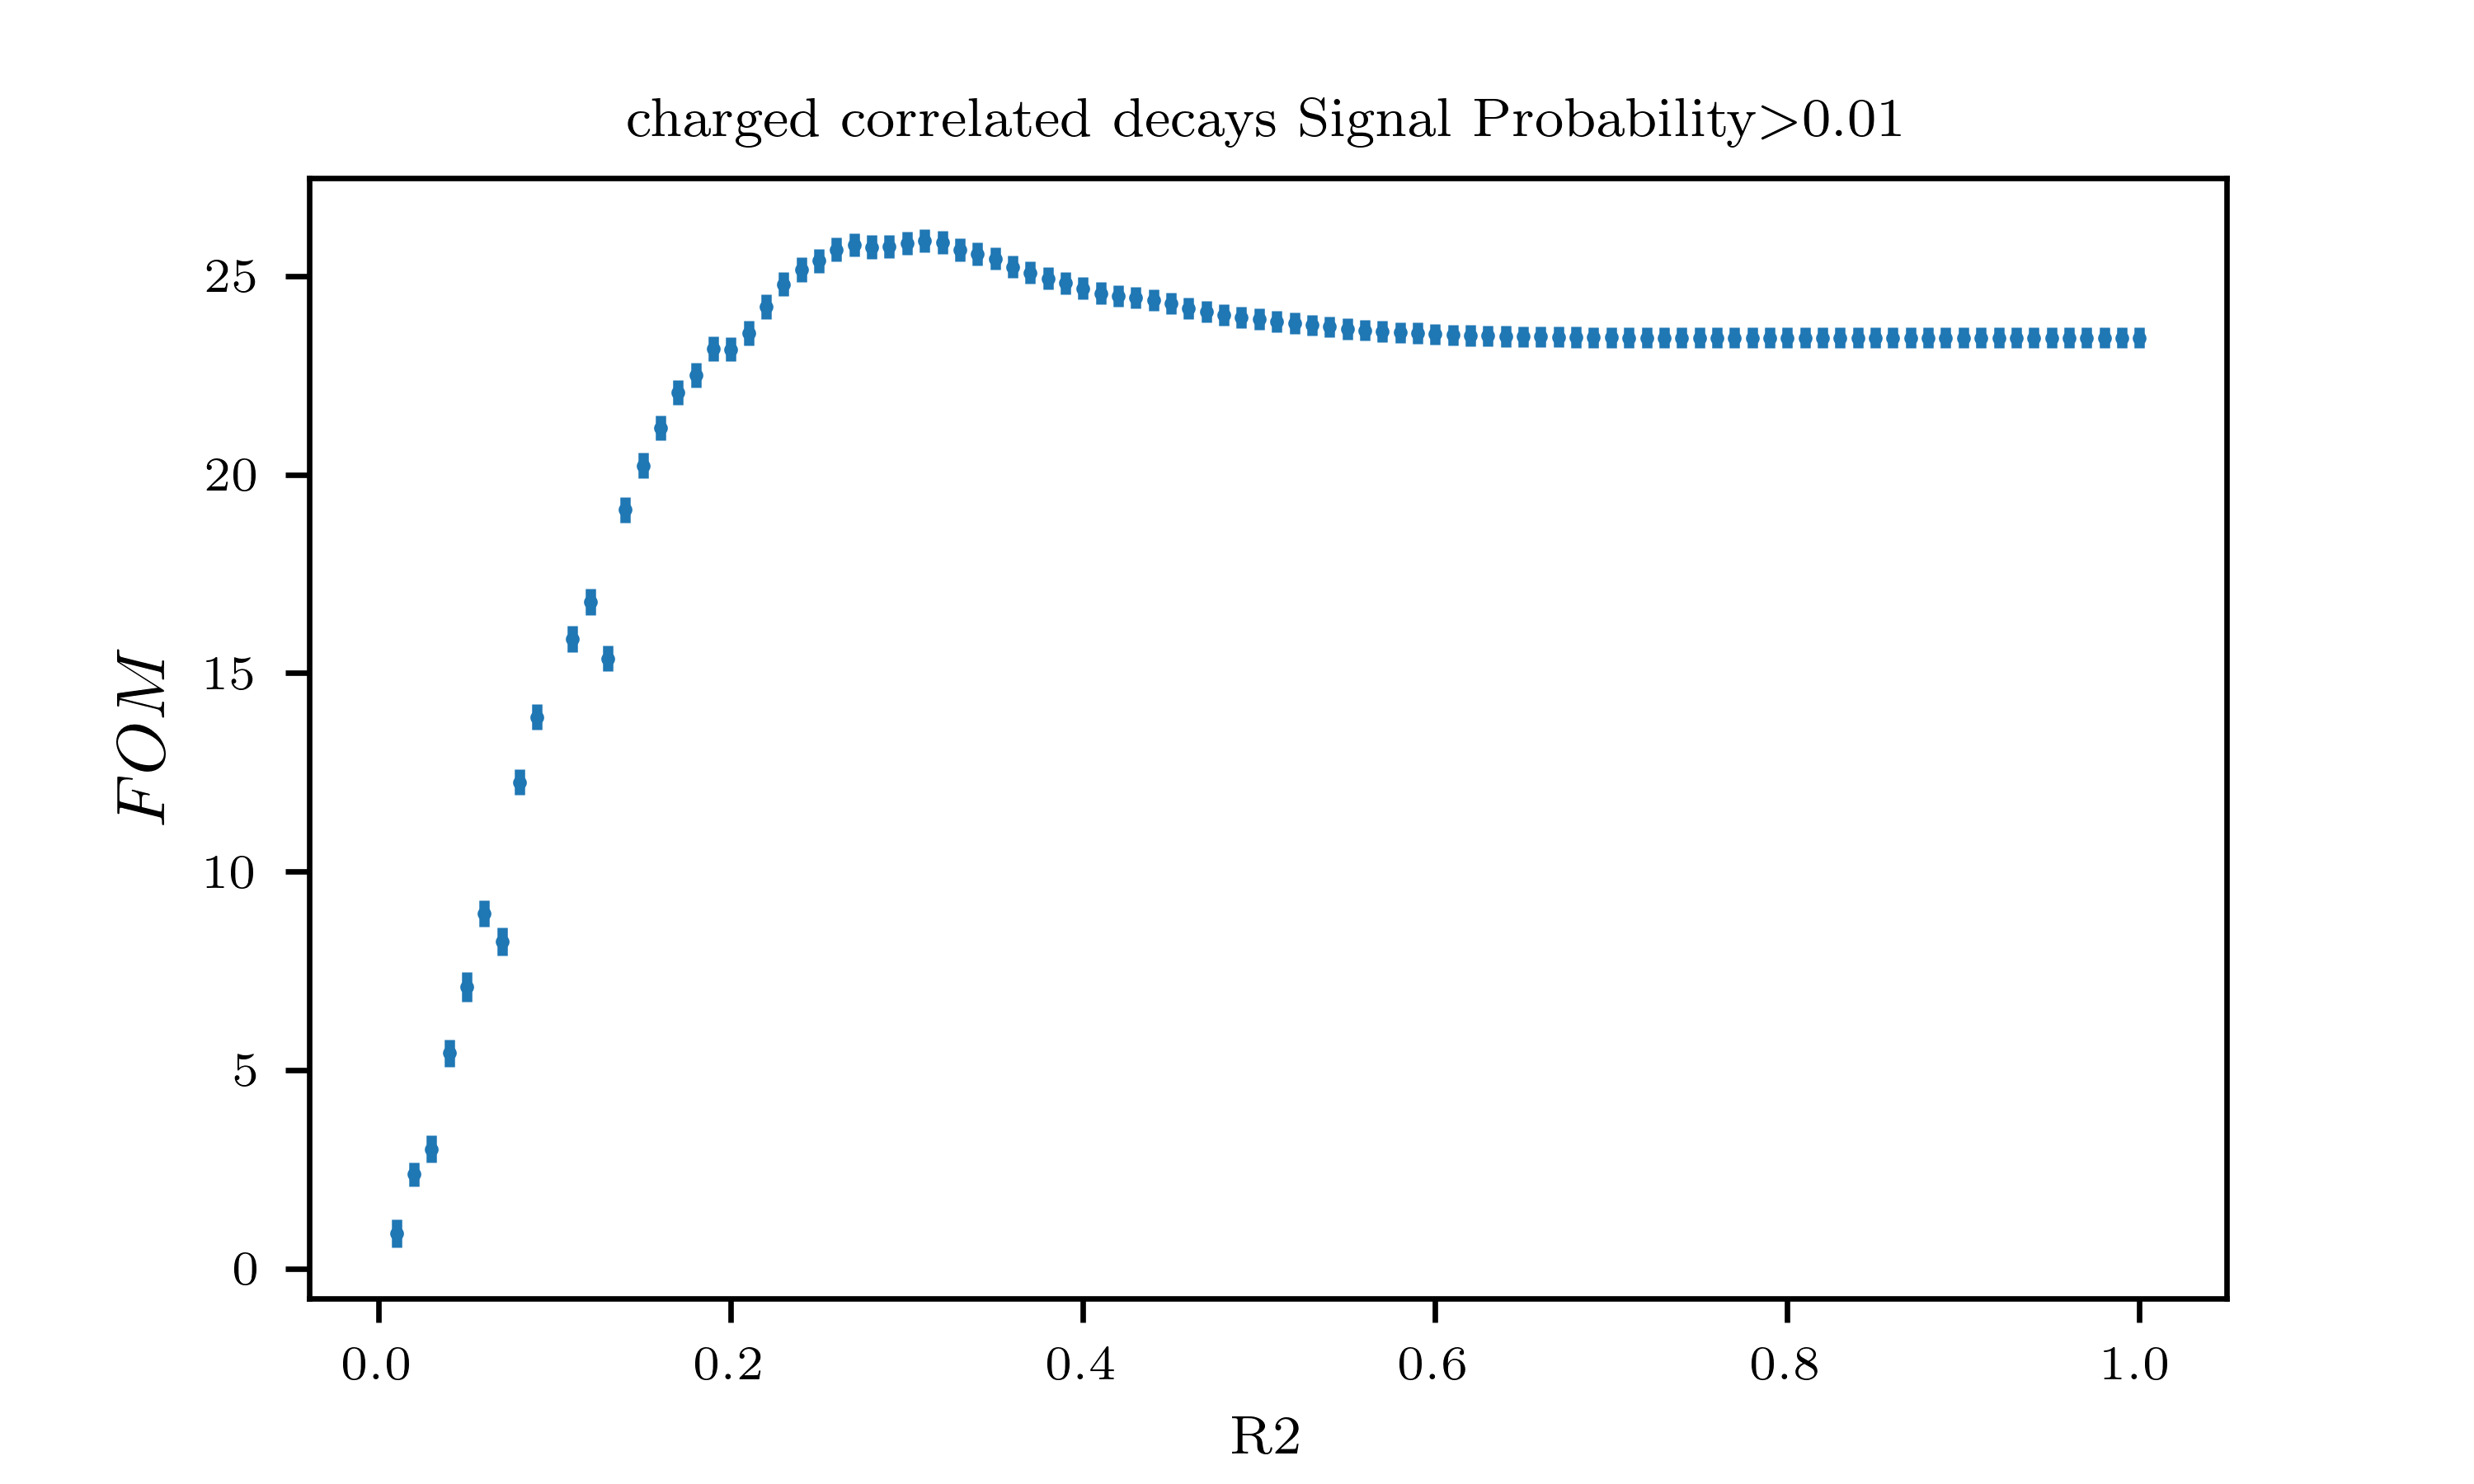
\includegraphics[width=0.75\textwidth]{03-Selection/figs/corr_chargedB_FOMvsR2_cut_SigProbOpt.png}}
\caption{Figure of Merit values calculated at several cuts on the $foxWolframR2$ variable}
\label{fig:corr_chargedB_FOMvsR2_cut_SigProbOpt}
\end{figure}

With the optimized cuts on SignalProbability and $foxWolframR2$ variable, the cut on $p^{\Lambda_c}_{CMS}$ is optimized\\
\vspace{0.2 cm}


\begin{figure}[H]
%\centering
{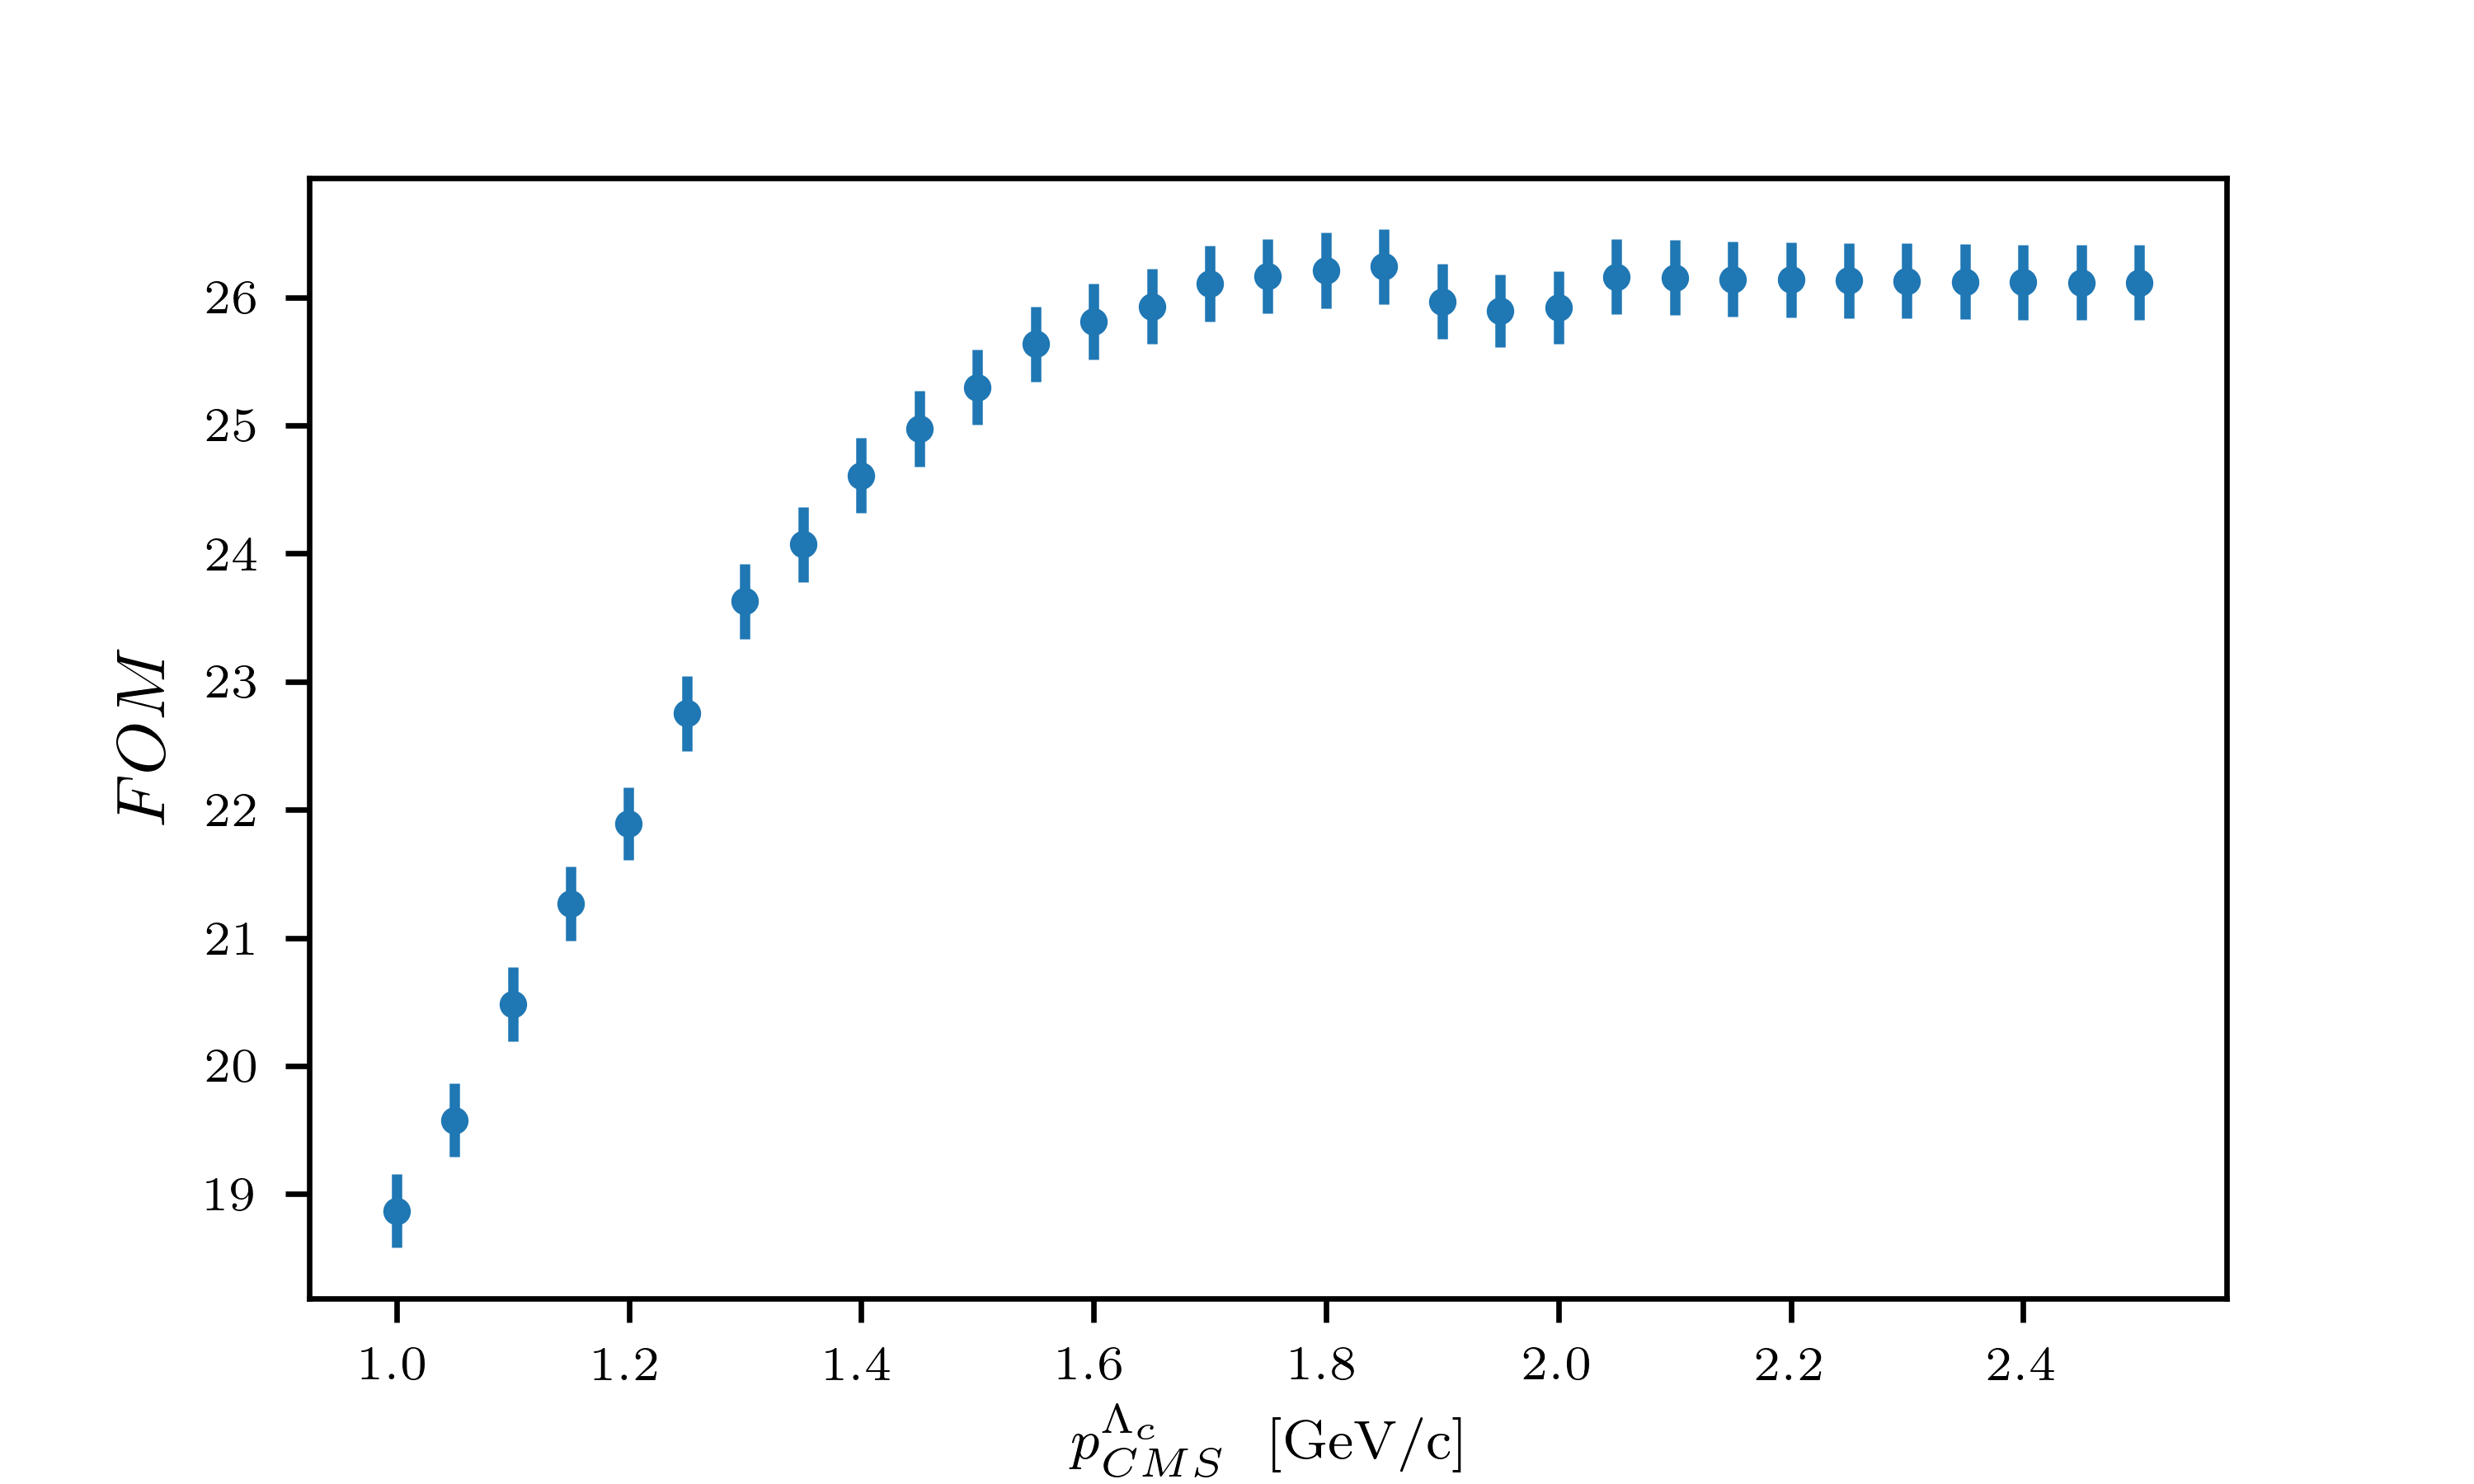
\includegraphics[width=0.85\textwidth]{03-Selection/figs/corr_chargedB_FOMvsCMS_Pcut.png}}
\caption{Figure of Merit values calculated at several cuts on the momentum of the $\Lambda_c$ candidates in the center of mass system}
\label{fig:corr_chargedB_FOMvsCMS_Pcut}
\end{figure}
From Fig. \ref{fig:corr_chargedB_FOMvsCMS_Pcut} one can see that with values of the cut above $p^{\Lambda_c}_{CMS} <$ 1.8 GeV/$c^2$ a plateau of maximum FOM values is reached. But such a cut would still be useful to reject some background events as one can see from Fig. \ref{fig:LogPlotchargedBcorr_Lambda_c_CMS_P_optimisedSigProb_R}.  \\
Finally the optimized selection cuts are:

\begin{itemize}
    \item $foxWolframR2  < $  0.3
    \item SignalProbability $>$ 0.01
    \item $p^{\Lambda_c}_{CMS} <$ 1.8 GeV/$c$
\end{itemize}


\begin{figure}[H]
%\centering
{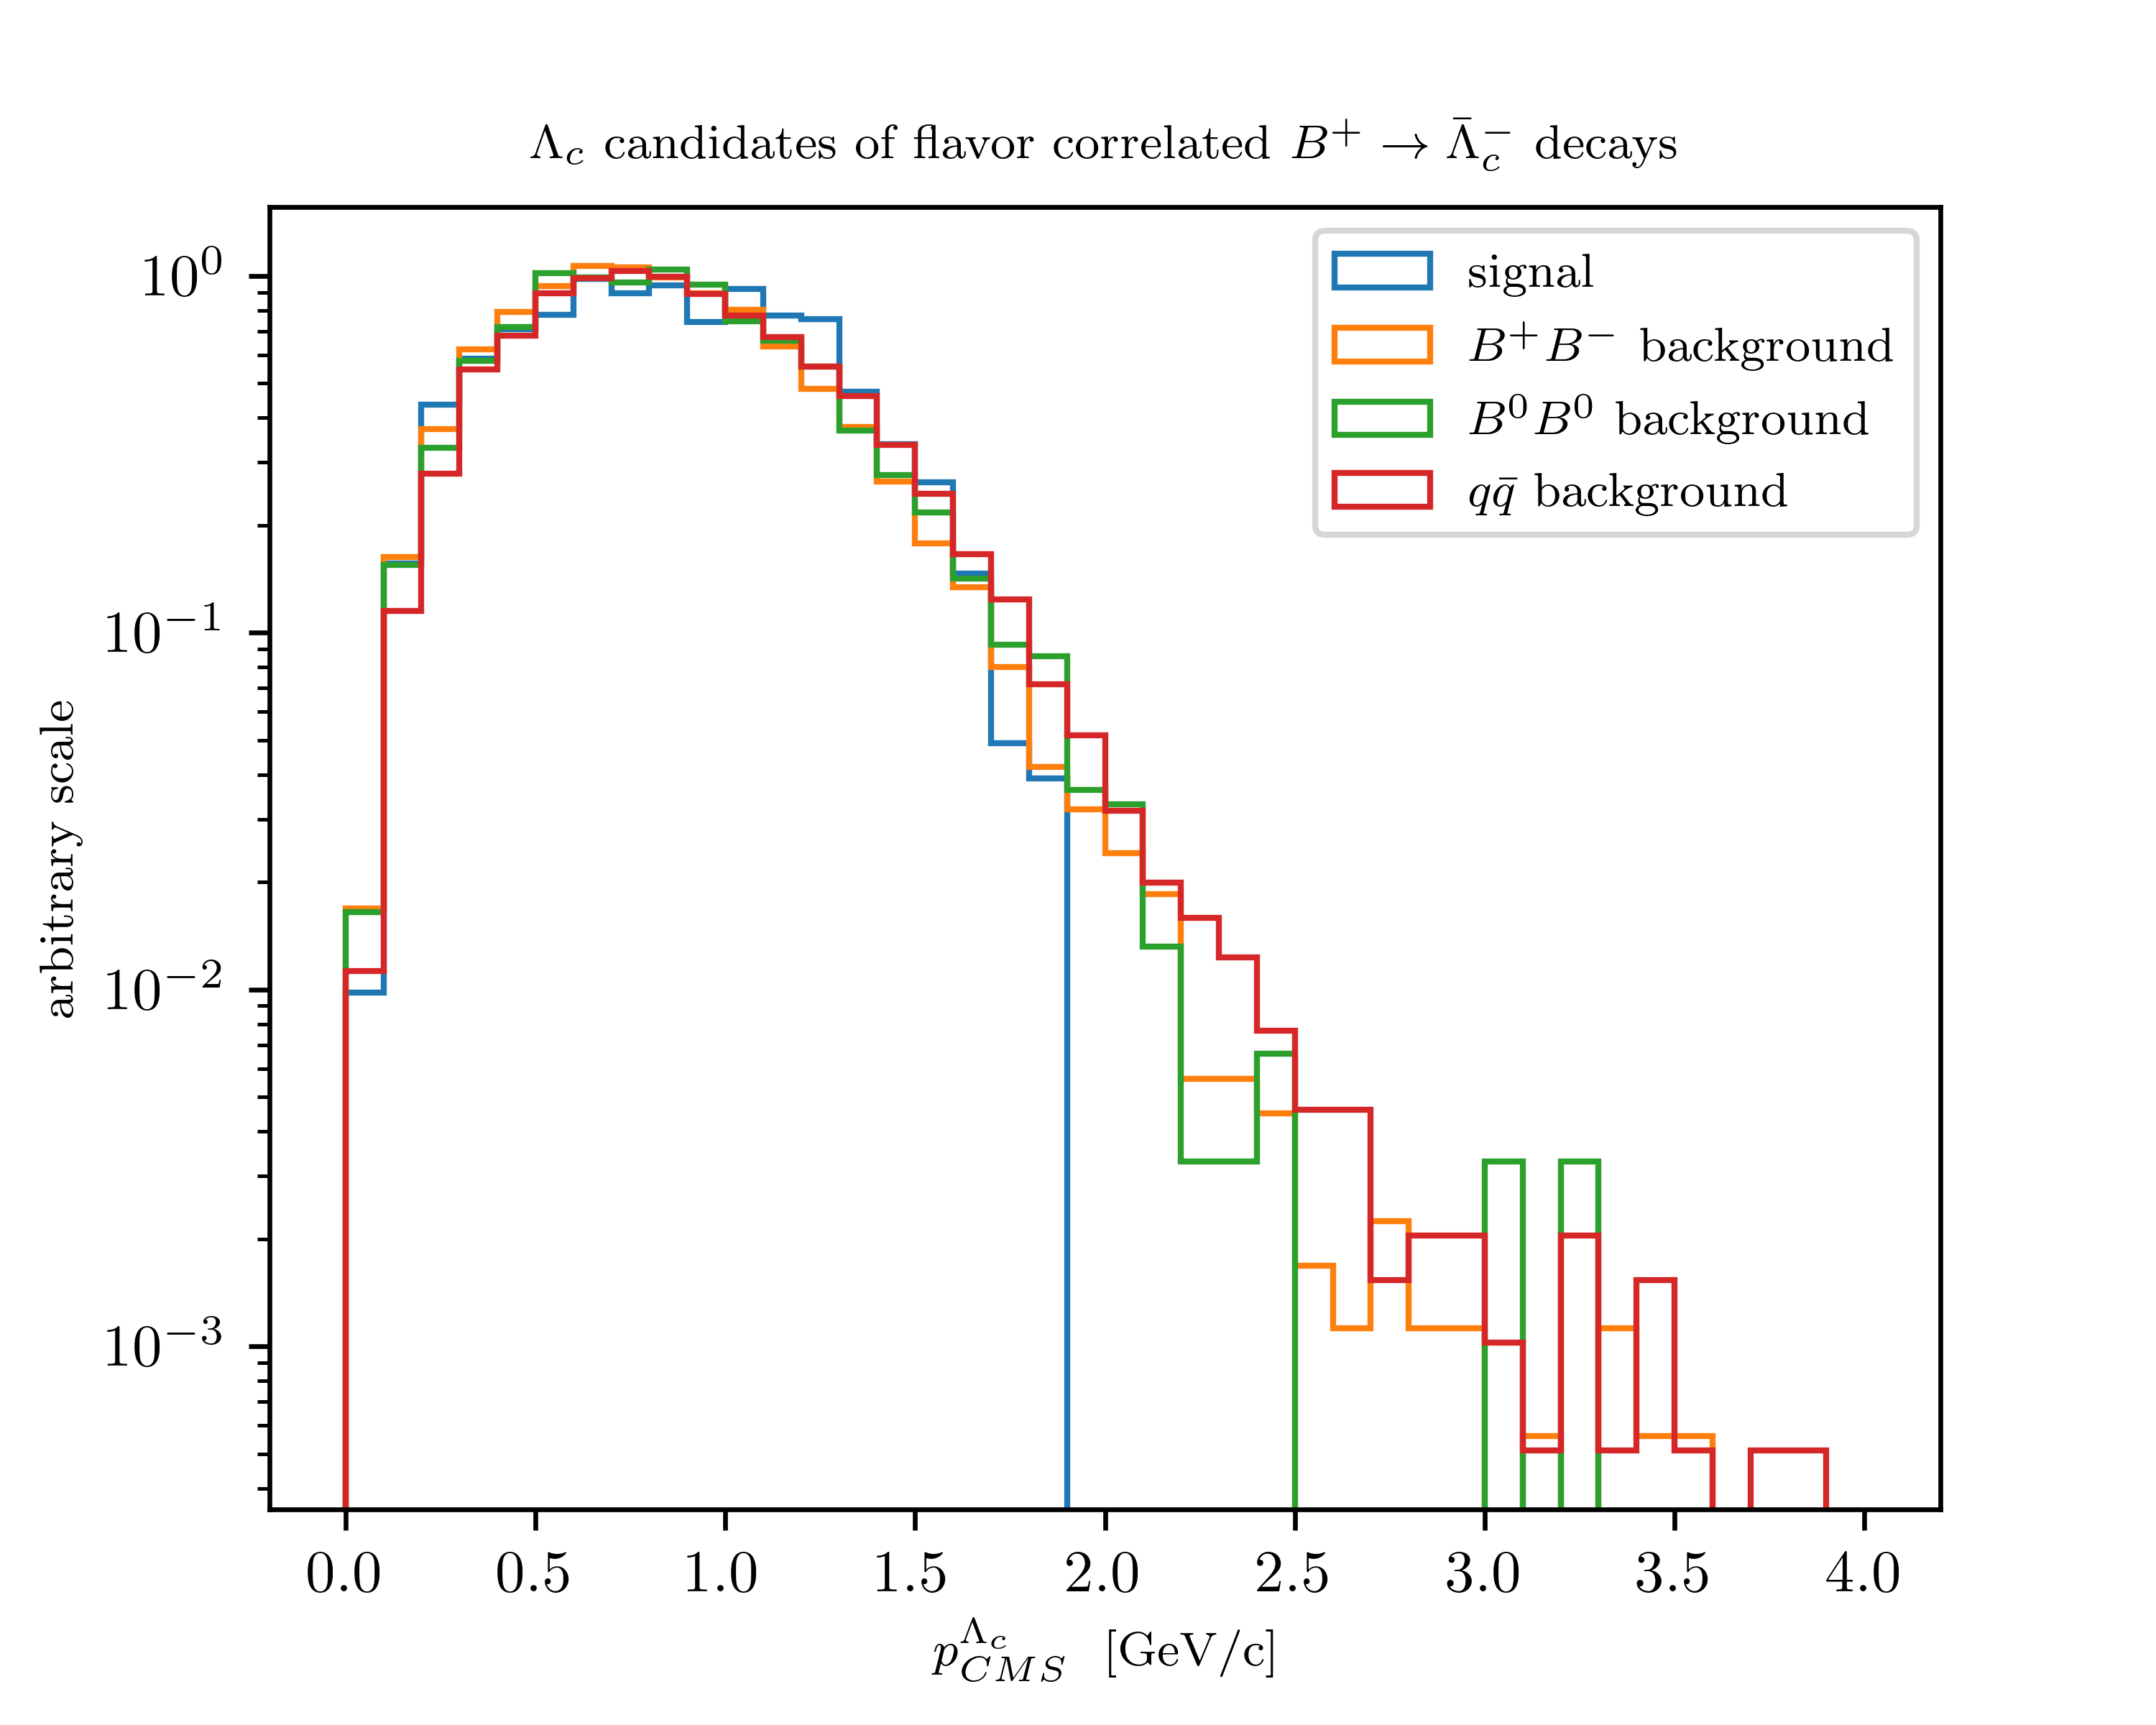
\includegraphics[width=0.85\textwidth]{03-Selection/figs/LogPlotchargedBcorr_Lambda_c_CMS_P_optimisedSigProb_R.png}}
\caption{Distribution of  $\Lambda_c$ candidates momenta in the center of mass system}
\label{fig:LogPlotchargedBcorr_Lambda_c_CMS_P_optimisedSigProb_R}
\end{figure}

\begin{figure}[h!]
%\centering
{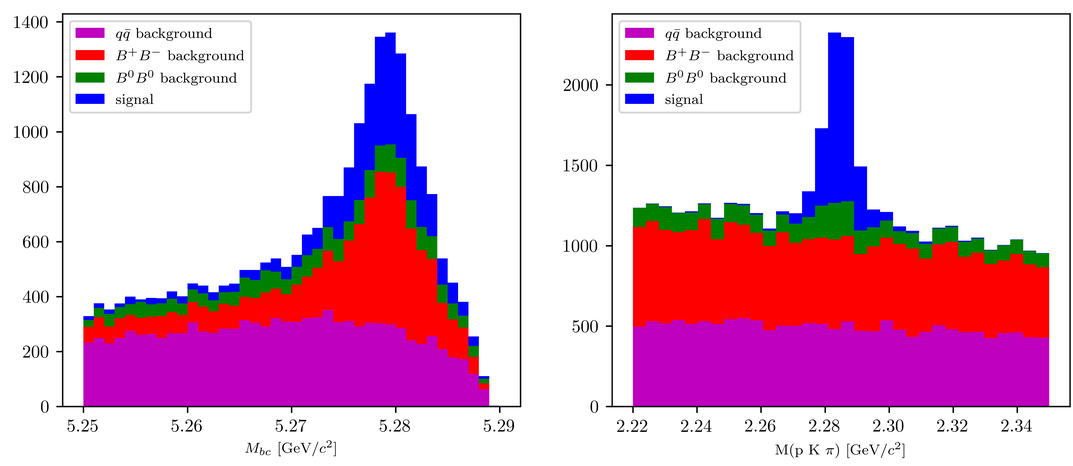
\includegraphics[width=0.95\textwidth]{03-Selection/figs/Mbc_InvM_optimizedSelection_SigR.png}}
\caption{Distribution of $M_{bc} $ (left) and invariant mass of charged correlated $\Lambda_c$  candidates (right), in the signal region after the above mentioned selection cuts.}
\label{fig:Mbc_InvM_optimizedSelection_SigR}
\end{figure}

\subsection{$B^+ \rightarrow \Lambda_c^+$ decays}
\label{sec:chargedAntiBtoLambdaC}

For anticorrelated decays, the same  $foxWolframR2$ cut is defined after the optimization procedure (see \cref{fig:acorr_chargedB_FOMvsR2_cut_SigProbOpt}).

\begin{figure}[h!]
    %\centering
    {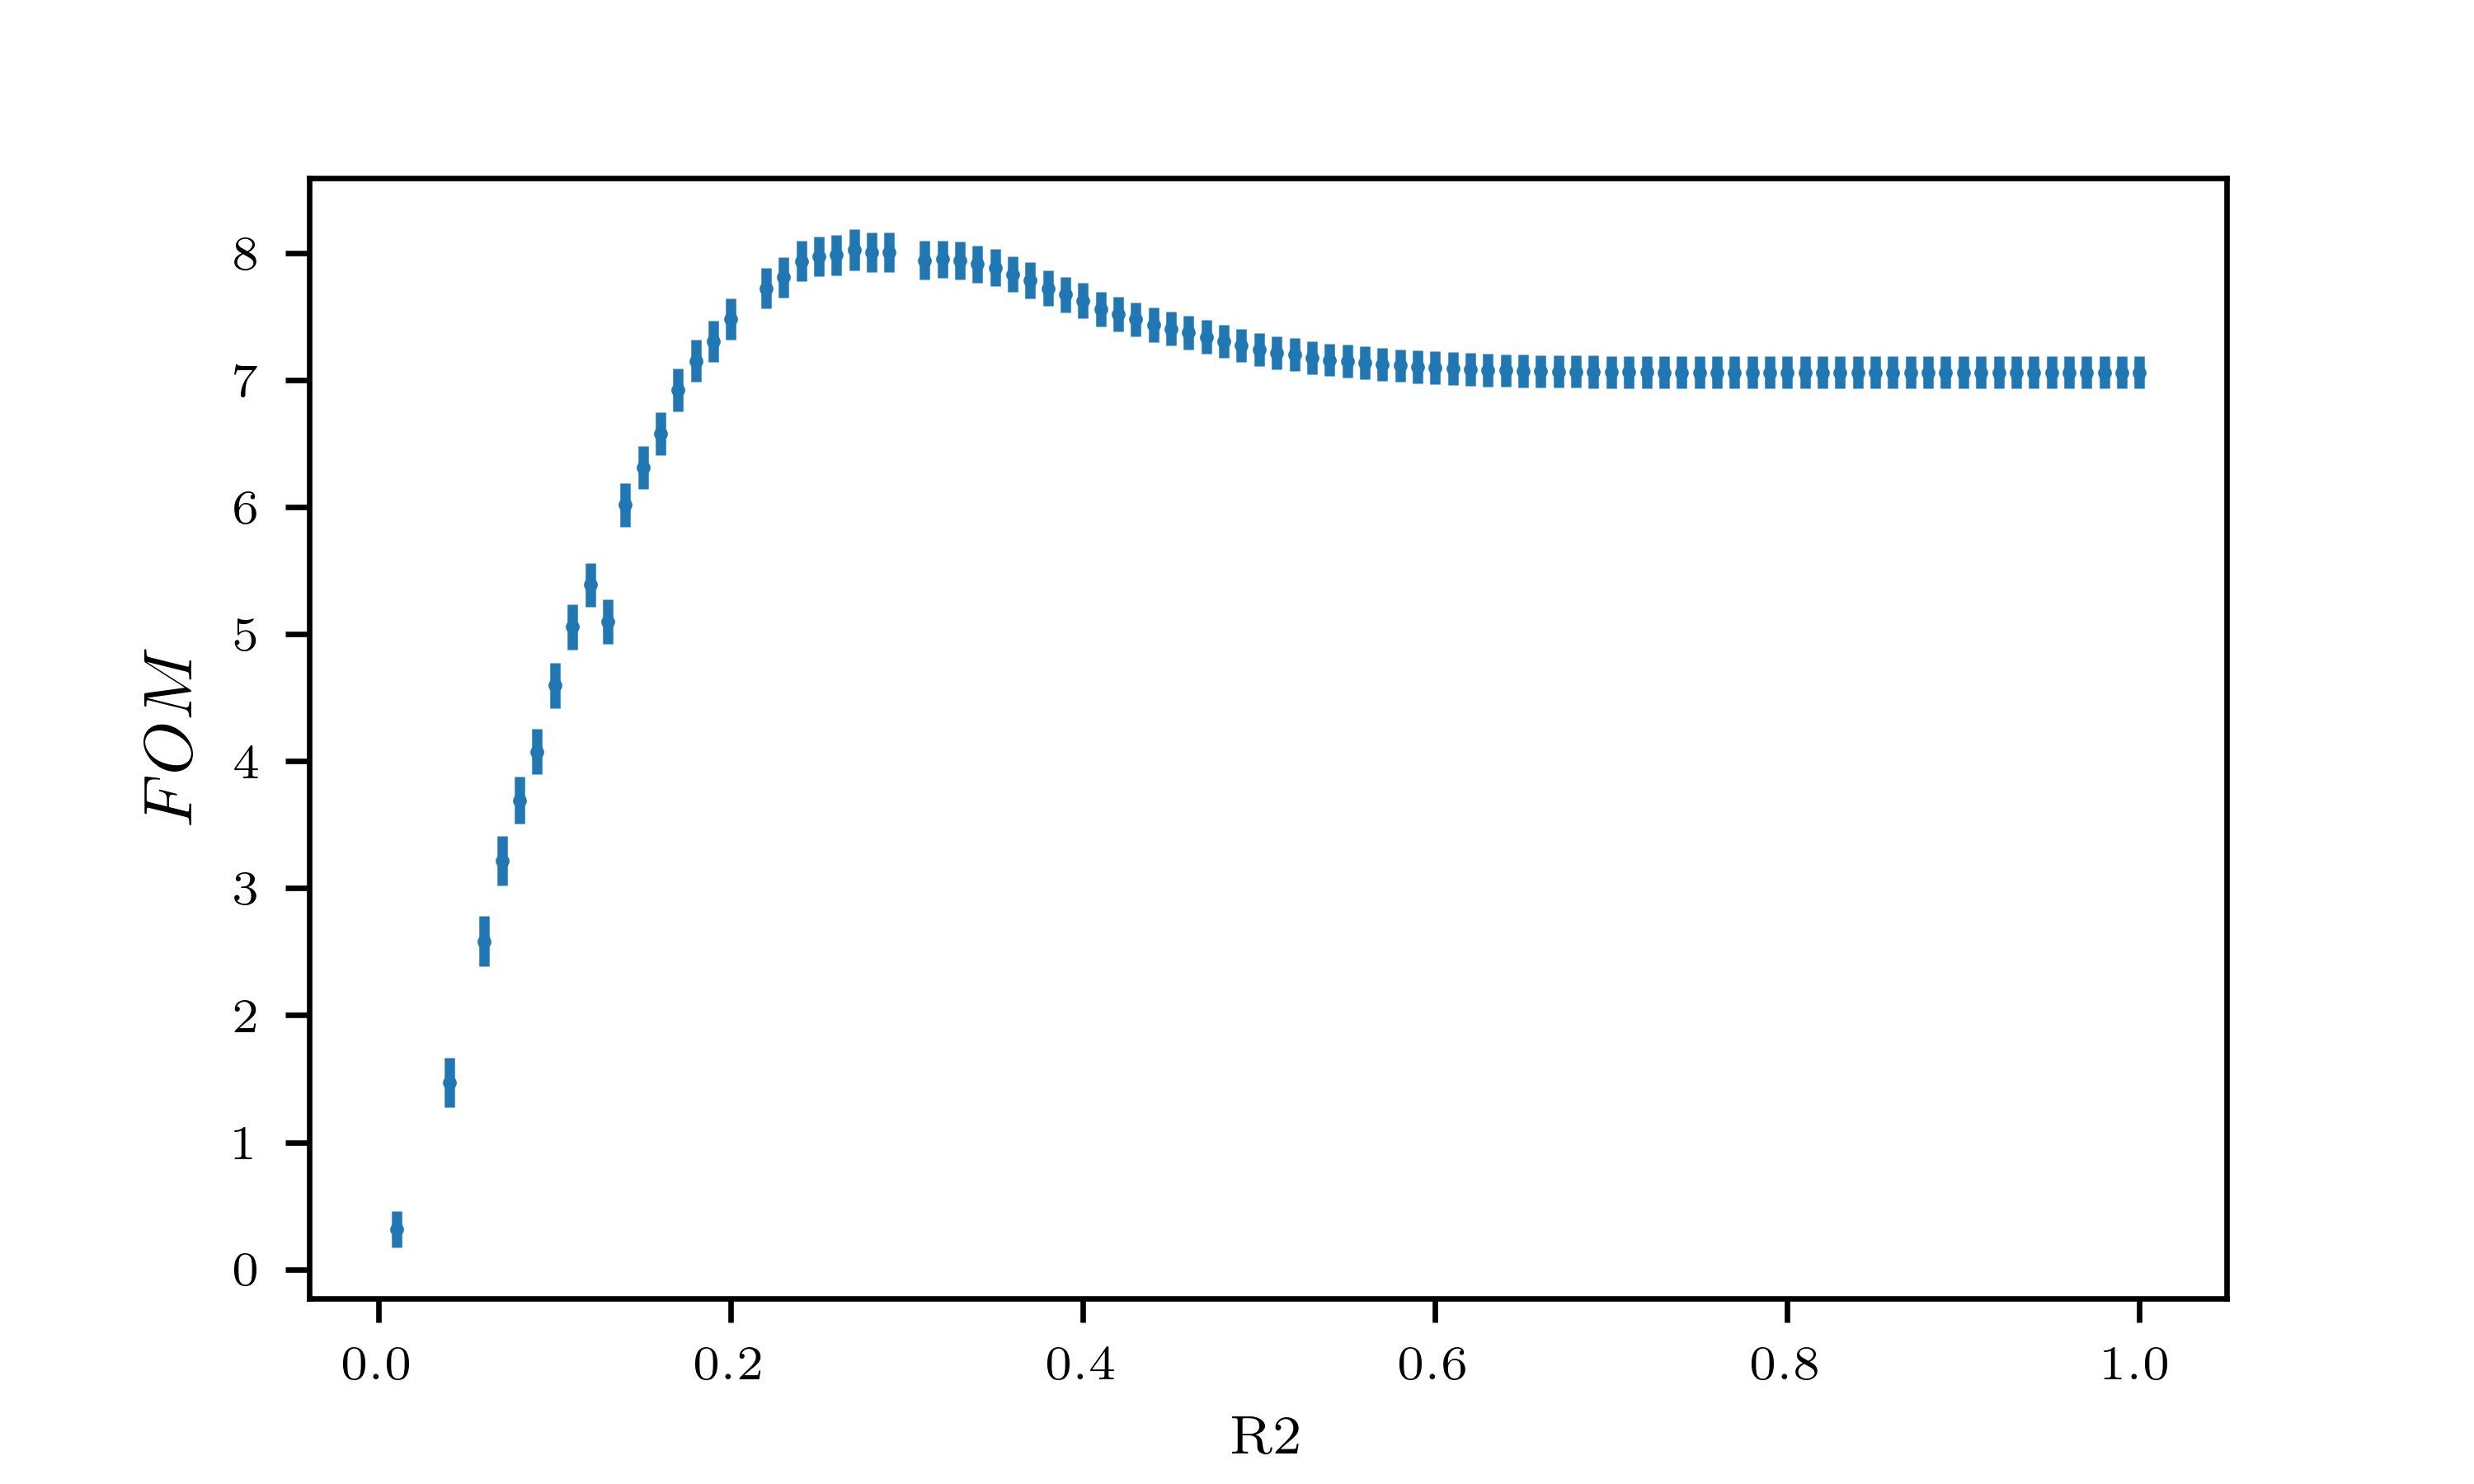
\includegraphics[width=0.65\textwidth]{03-Selection/figs/acorr_chargedB_FOMvsR2_cut.png}}
    \caption{Figure of Merit values calculated at several cuts on the $foxWolframR2$ variable}
    \label{fig:acorr_chargedB_FOMvsR2_cut}
    \end{figure}

\begin{figure}[H]
    %\centering
    {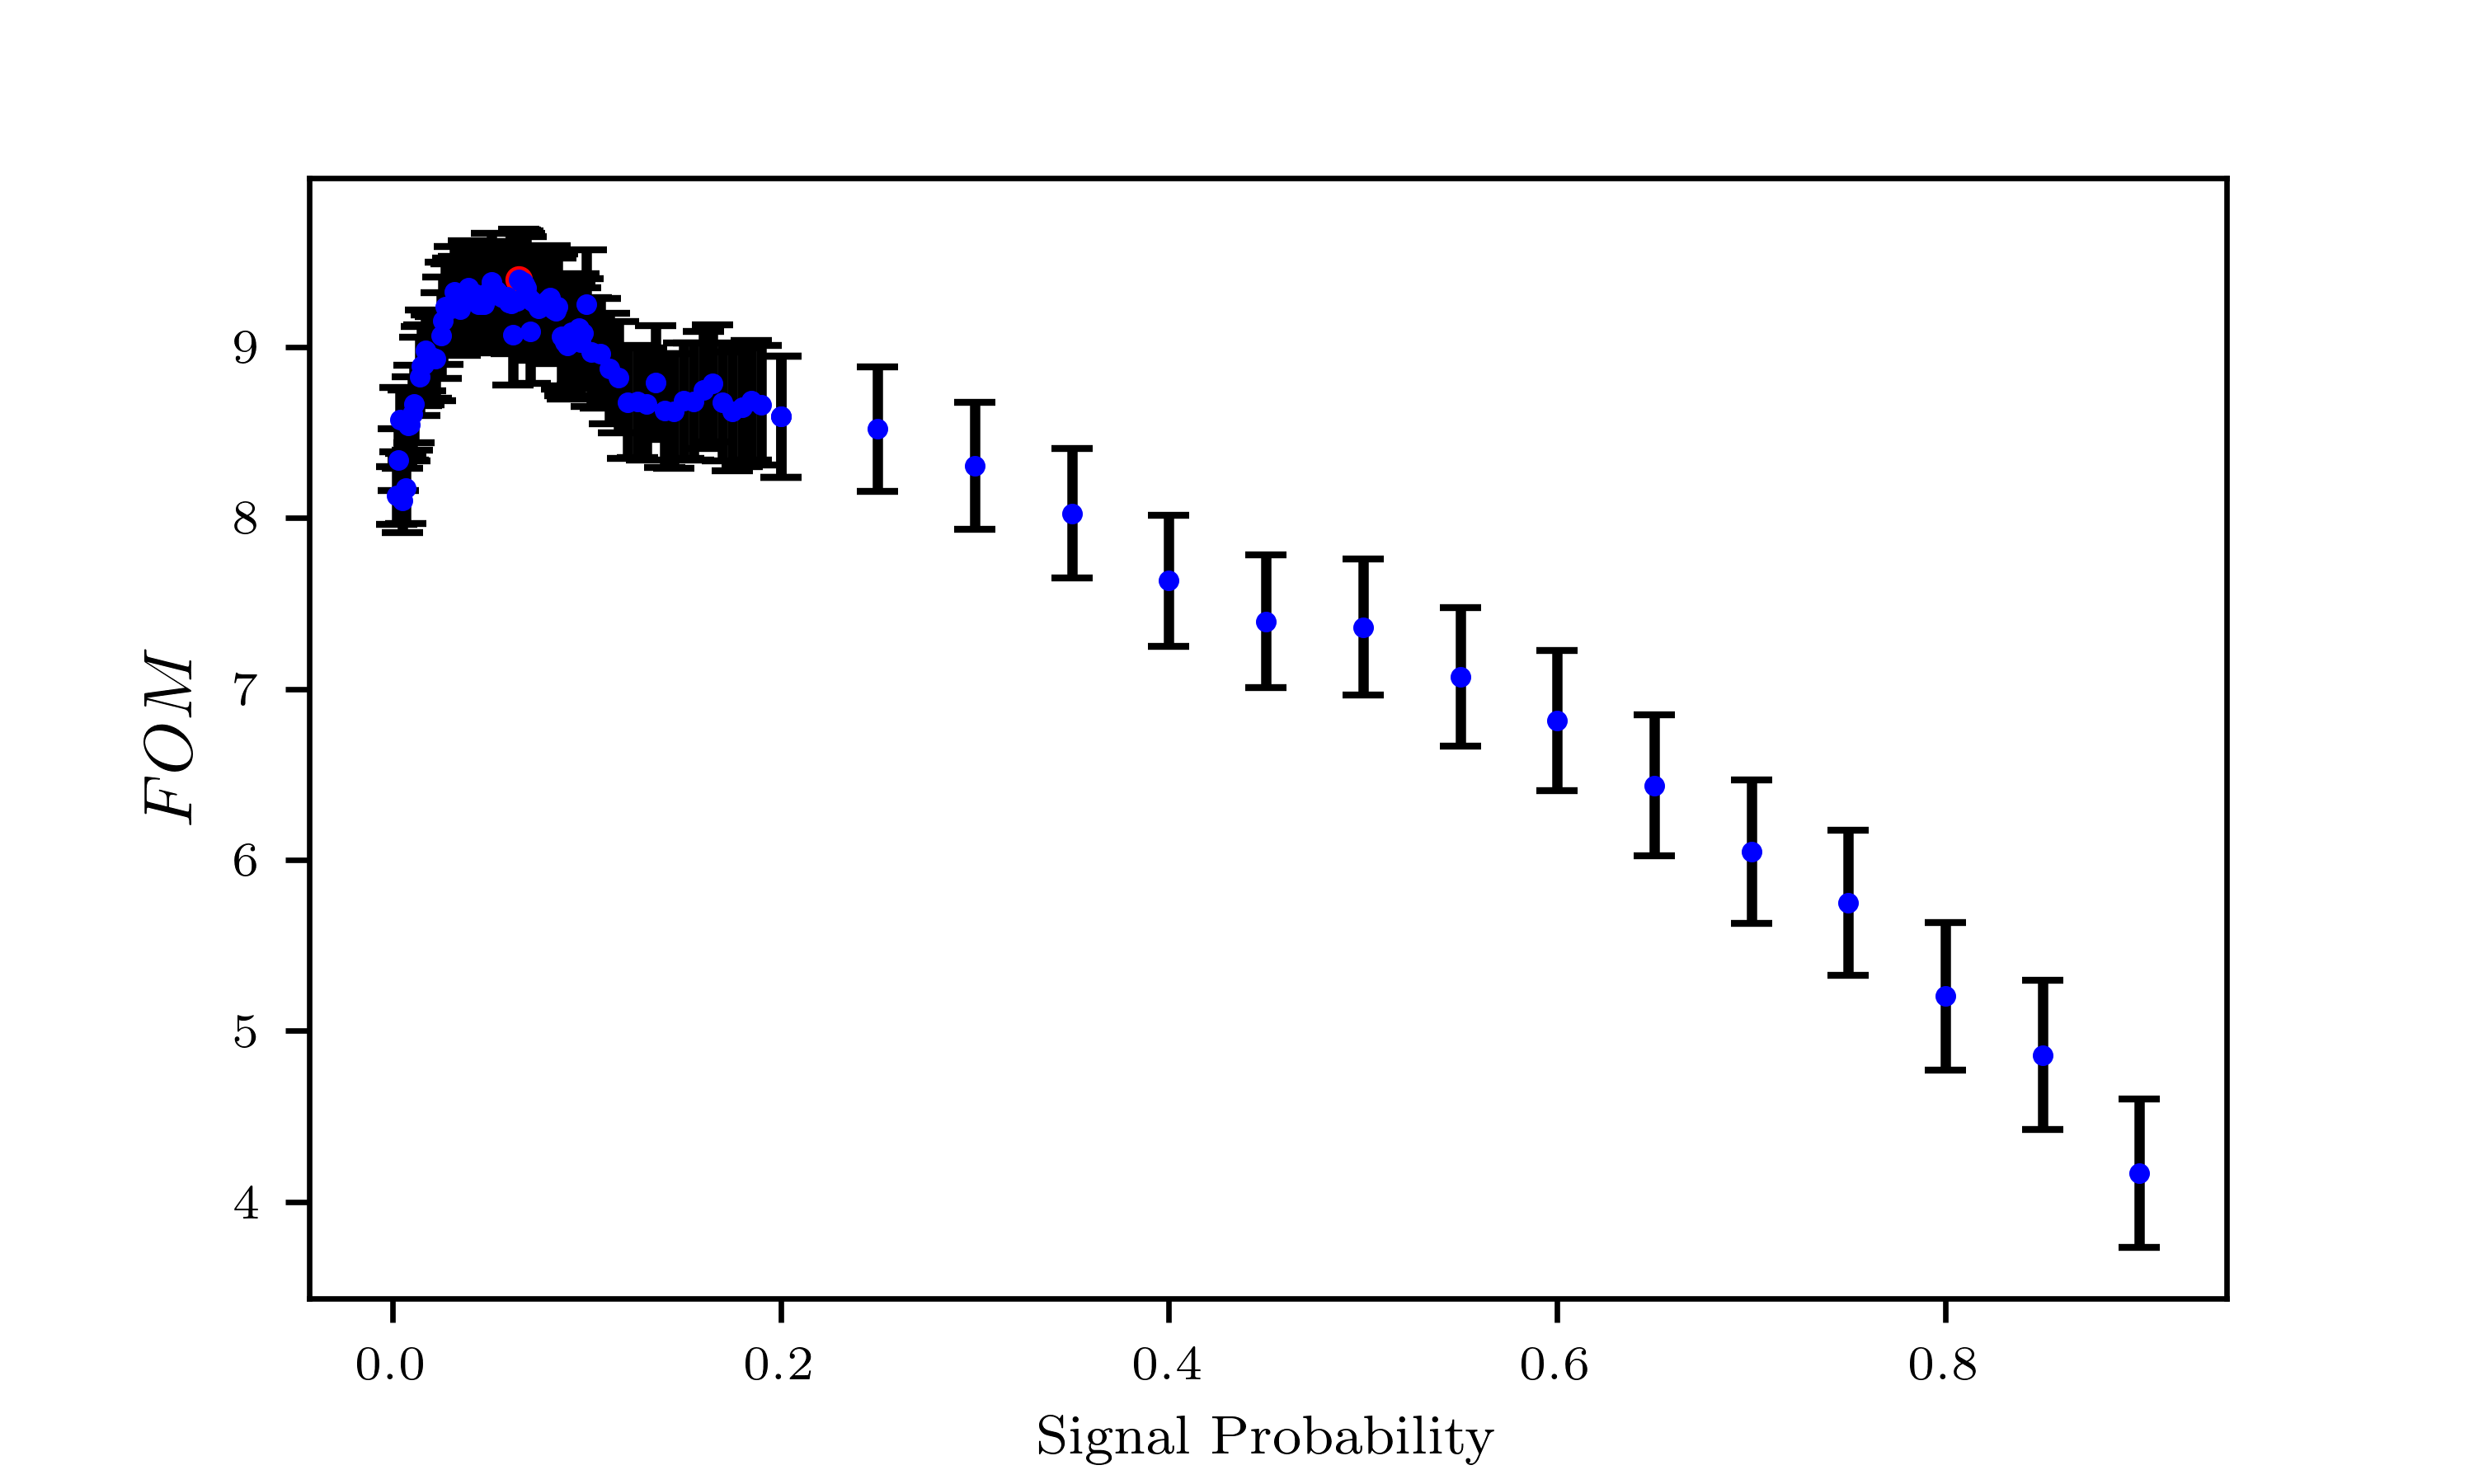
\includegraphics[width=0.75\textwidth]{03-Selection/figs/charged_anticorrLambdaC_FOMvsSigProb.png}}
    \caption{Figure of Merit values calculated at several cuts on the SignalProbability variable}
    \label{fig:charged_anticorrLambdaC_FOMvsSigProb}
    \end{figure}



\begin{figure}[H]
    %\centering
    {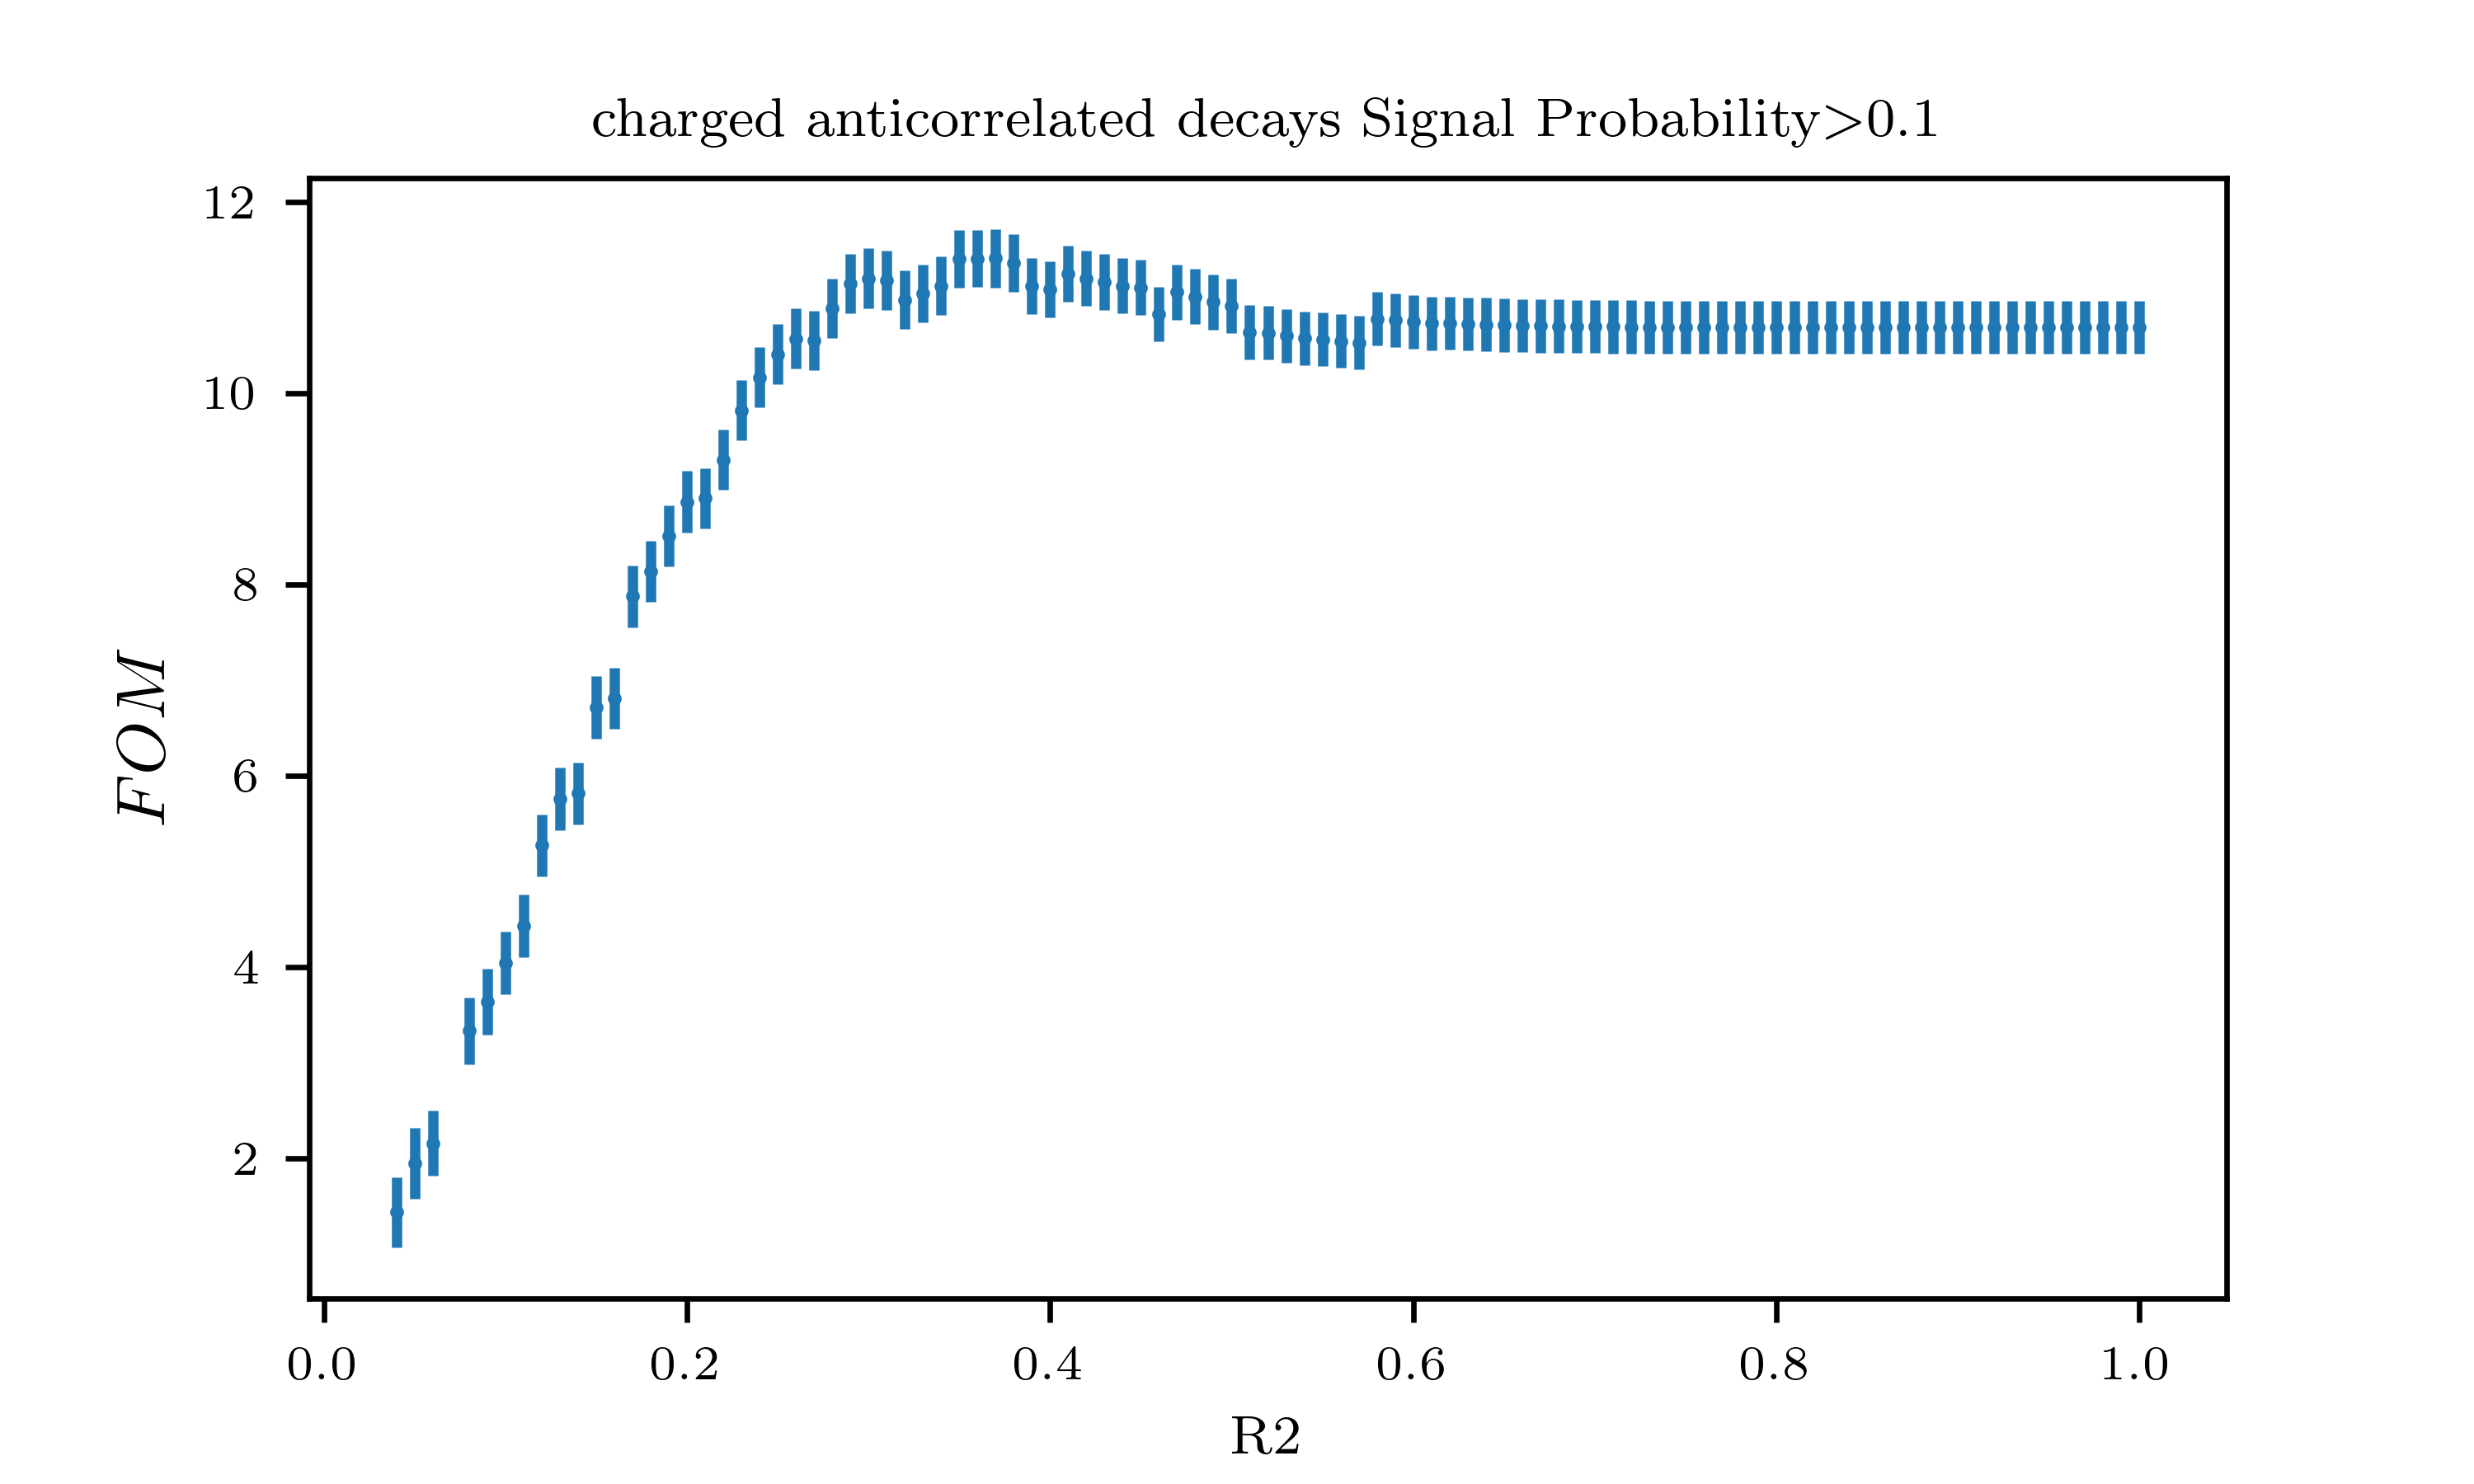
\includegraphics[width=0.75\textwidth]{03-Selection/figs/acorr_chargedB_FOMvsR2_cut_SigProbOpt.png}}
    \caption{Figure of Merit values calculated at several cuts on the $foxWolframR2$ variable}
    \label{fig:acorr_chargedB_FOMvsR2_cut_SigProbOpt}
    \end{figure}


    With the optimized cuts on SignalProbability and $foxWolframR2$ variable, the cut on $p^{\Lambda_c}_{CMS}$ is selected.\\
    \vspace{0.2 cm}
    

    \begin{figure}[H]
        %\centering
        {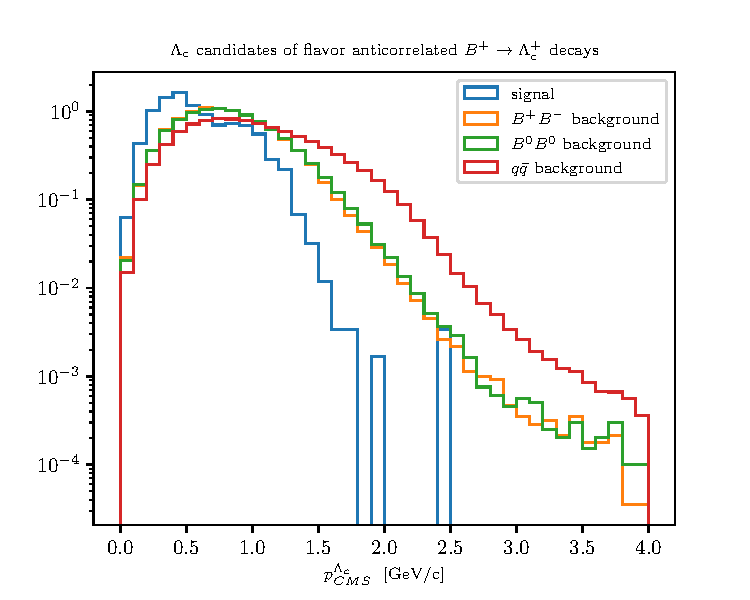
\includegraphics[width=0.85\textwidth]{03-Selection/figs/acorr_chargedB_Lambda_c_CMS_P.pdf}}
        \caption{Distribution of  $\Lambda_c$ candidates momenta in the center of mass system}
        \label{fig:acorr_chargedB_Lambda_c_CMS_P}
        \end{figure}
        
The final optimized selection cuts are:

        \begin{itemize}
            \item $foxWolframR2  < $  0.3
            \item SignalProbability $>$ 0.1
            \item $p^{\Lambda_c}_{CMS} <$ 1.5 GeV/$c$
        \end{itemize}
        
\cref{fig:acorr_chargedBMbc_InvM_optimizedSelection_SigR} shows the projections of the $M_{bc} $ and $M(p K \pi)$ distributions.

        \begin{figure}[H]
            %\centering
            {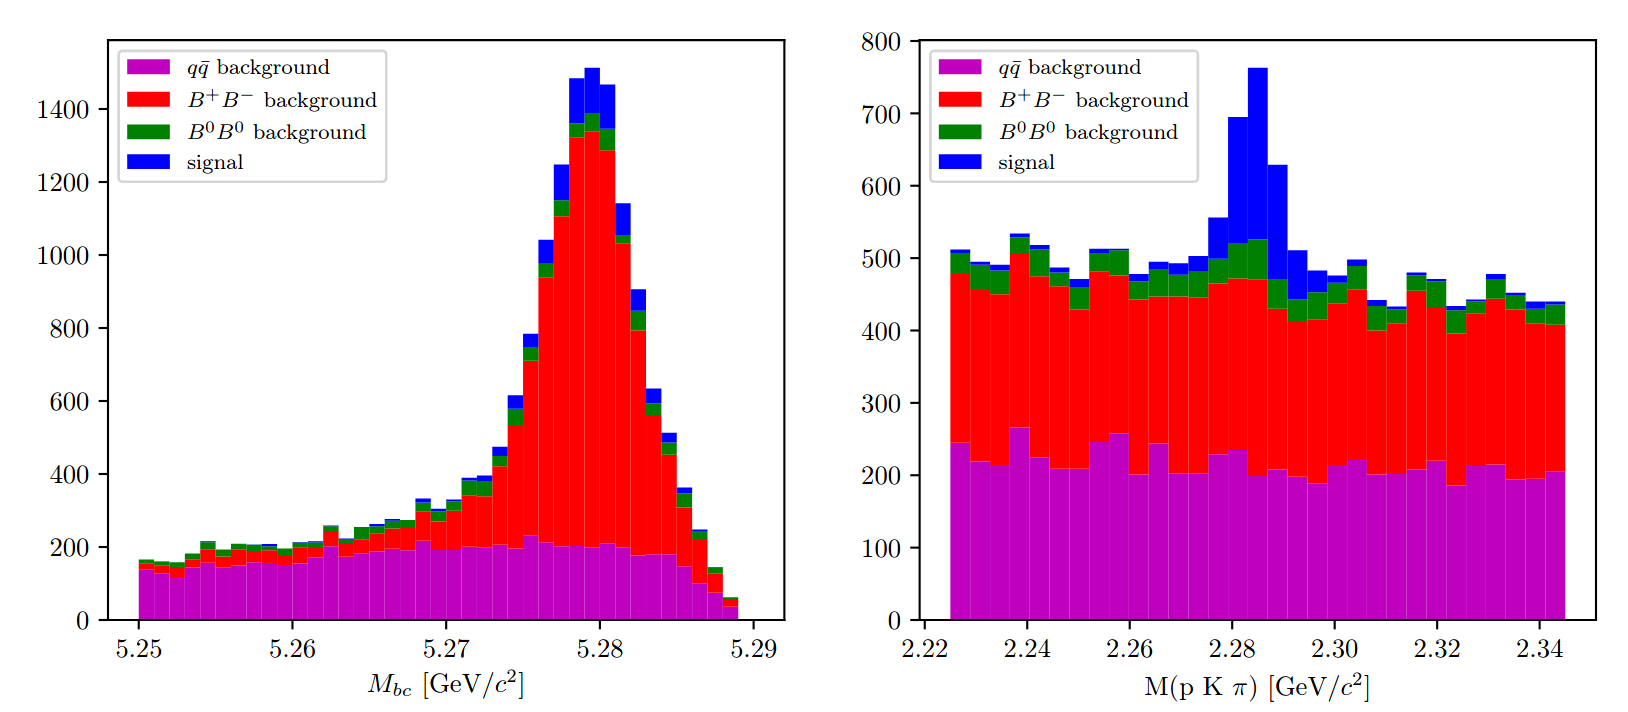
\includegraphics[width=0.95\textwidth]{03-Selection/figs/acorr_chargedB_Mbc_InvM_opt_cuts.png}}
            \caption{Distribution of $M_{bc} $ (left) and invariant mass of charged correlated $\Lambda_c$  candidates (right), in the signal region after the above mentioned selection cuts.}
            \label{fig:acorr_chargedBMbc_InvM_optimizedSelection_SigR}
            \end{figure}
               


\subsection{$\bar{B^0} \rightarrow \Lambda_c^+$ decays}
\label{sec:neutralCorrBtoLambdaC}

Also for neutral correlated decays, first  the cut on $foxWolframR2$ is optimized. 

\begin{figure}[h!]
    %\centering
    {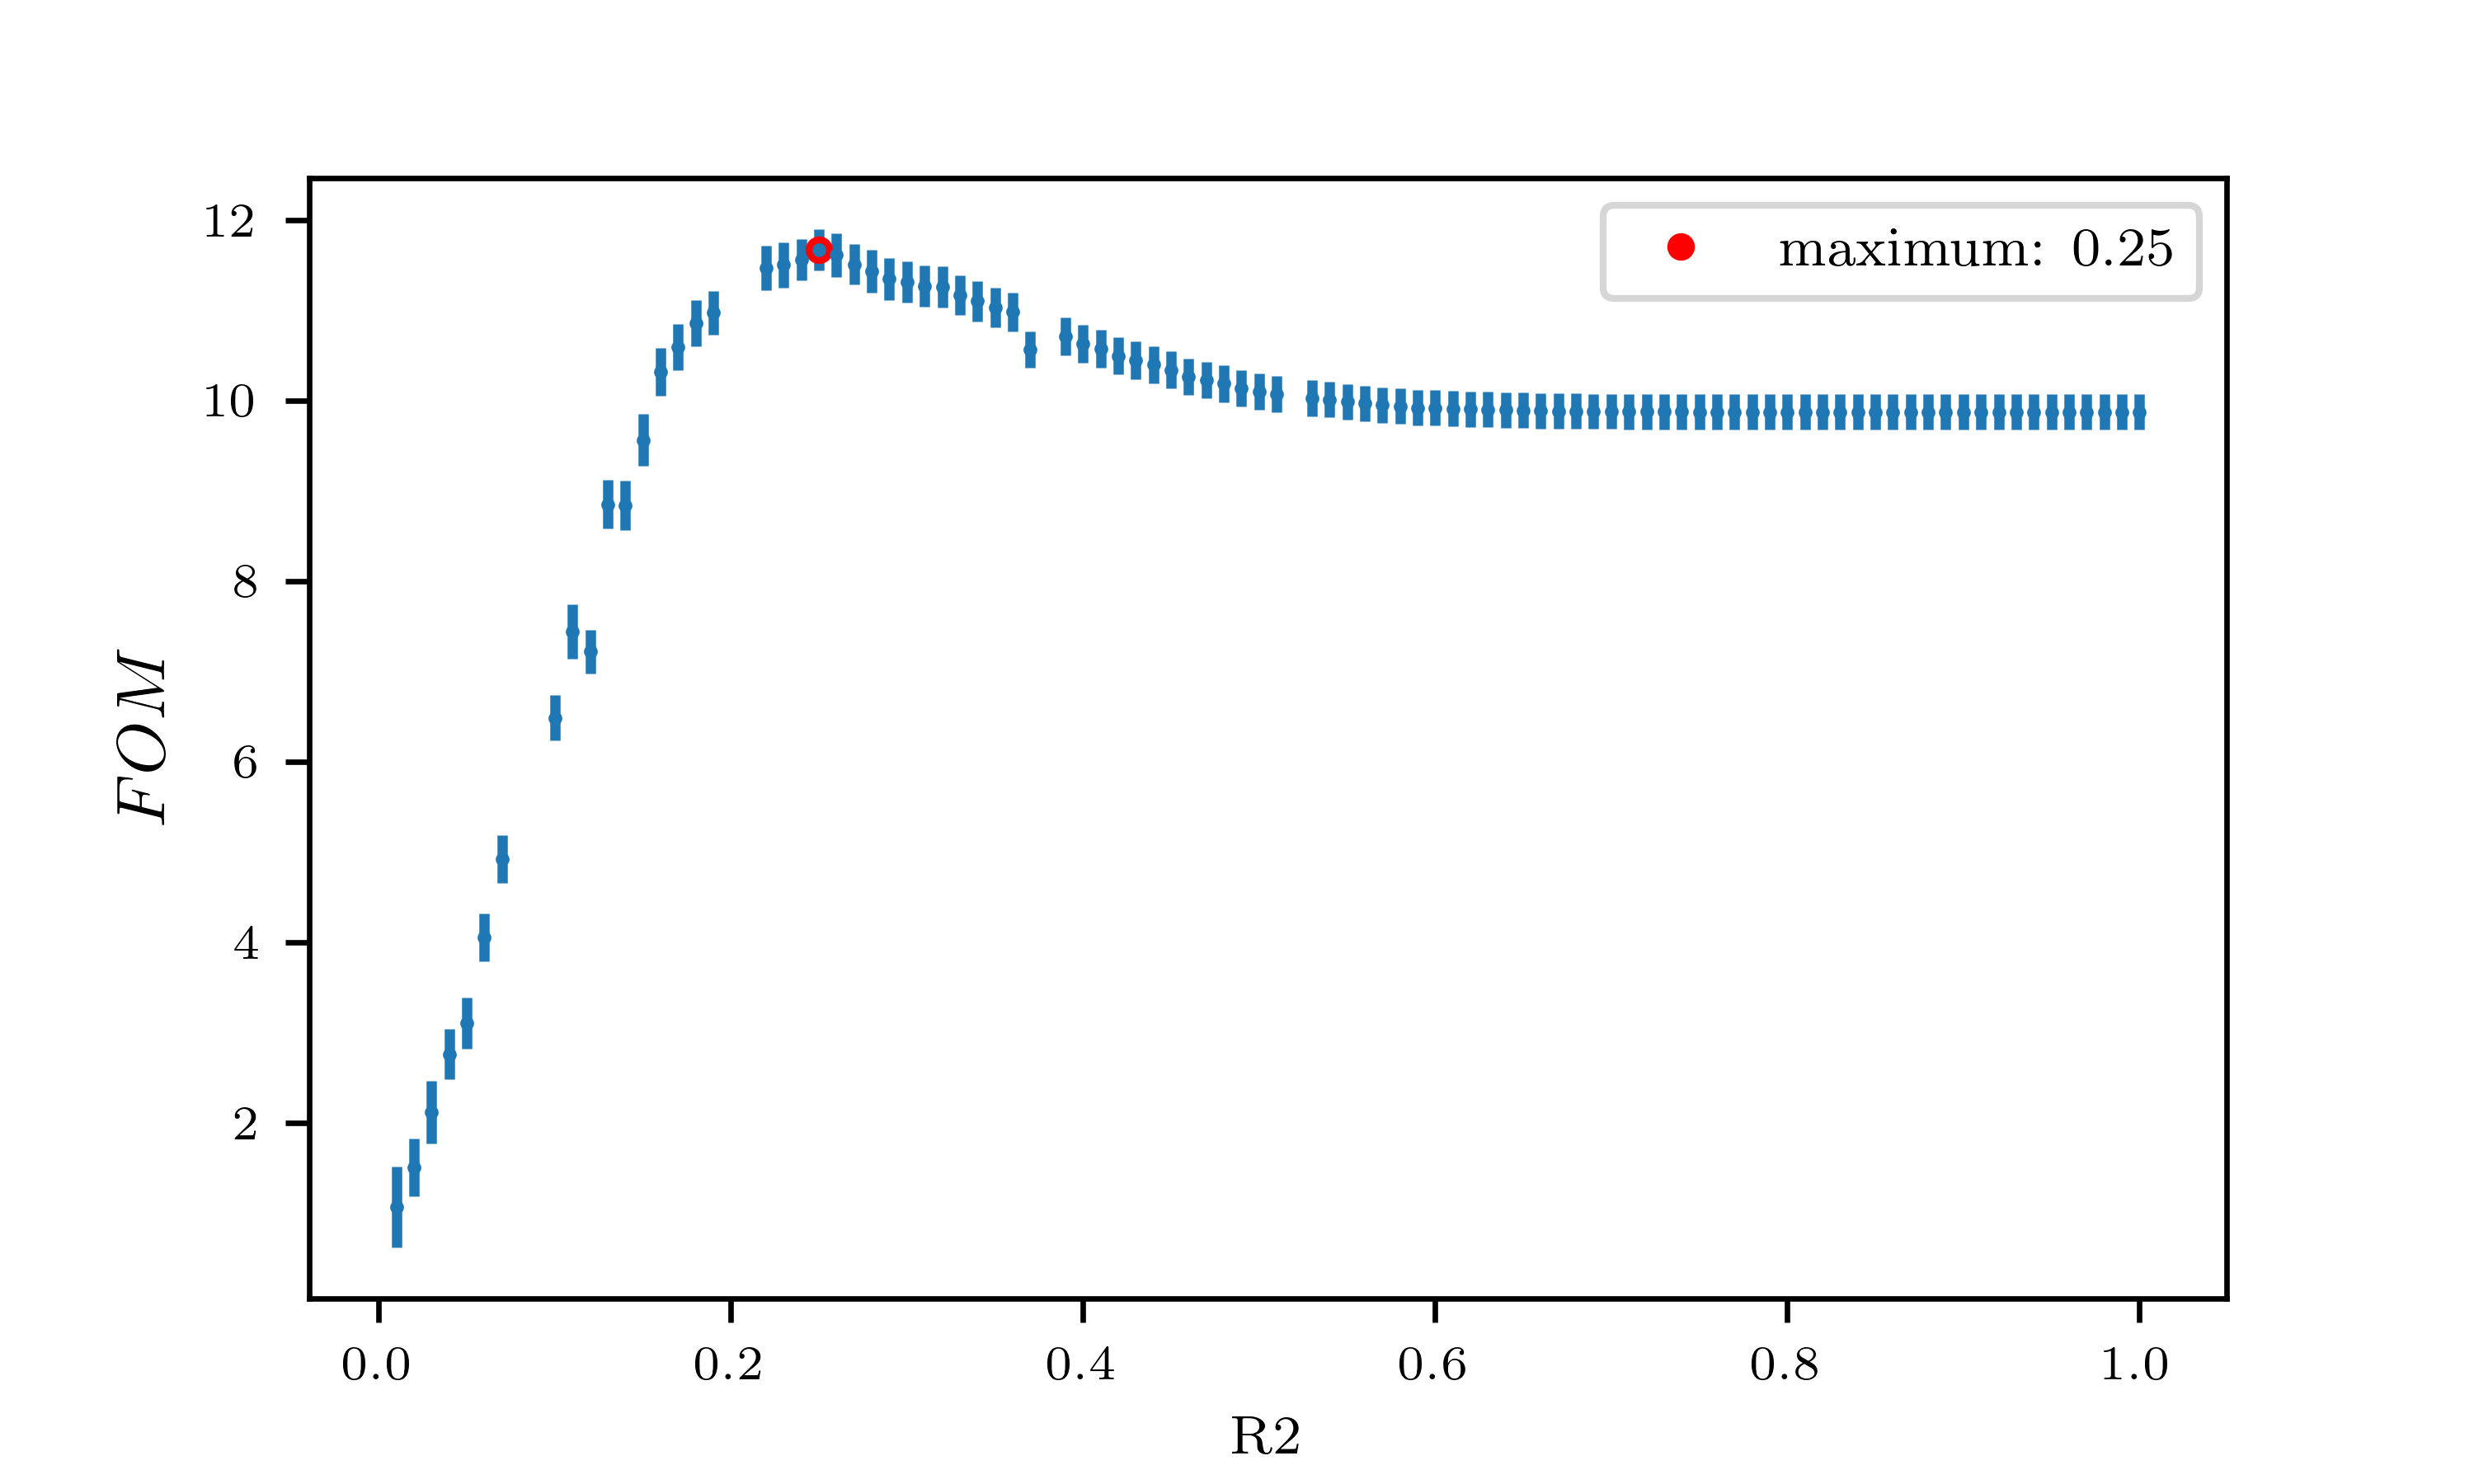
\includegraphics[width=0.65\textwidth]{03-Selection/figs/corr_B0_FOMvsR2_cut.png}}
    \caption{Figure of Merit values calculated at several cuts on the $foxWolframR2$ variable}
    \label{fig:corr_B0_FOMvsR2_cut}
    \end{figure}

    The cut suggested by \cref{fig:corr_B0_FOMvsR2_cut},  $foxWolframR2 < 0.27$ , is used to define the cut on the
    SignalProbability variable. From \cref{fig:corr_B0_FOMvsSigProb_cut_until1}, it seems the optimal cut maximazing
the $FOM$ would be around 0.05. If one zooms like in \cref{fig:B0corrLambdaC_FOMvsSigProb} one can see that there is a 
sort of plateau starting around  0.03 and ending after values around 0.11, where the values fluctuate within statistical 
uncertainties around $FOM$ = 13. In this case, a legitimate choice is to use the most stringent cut (SignalProbability > 0.11) 
being the $FOM$ same but rejecting more background events.
    
    

\begin{figure}[H]
    %\centering
    {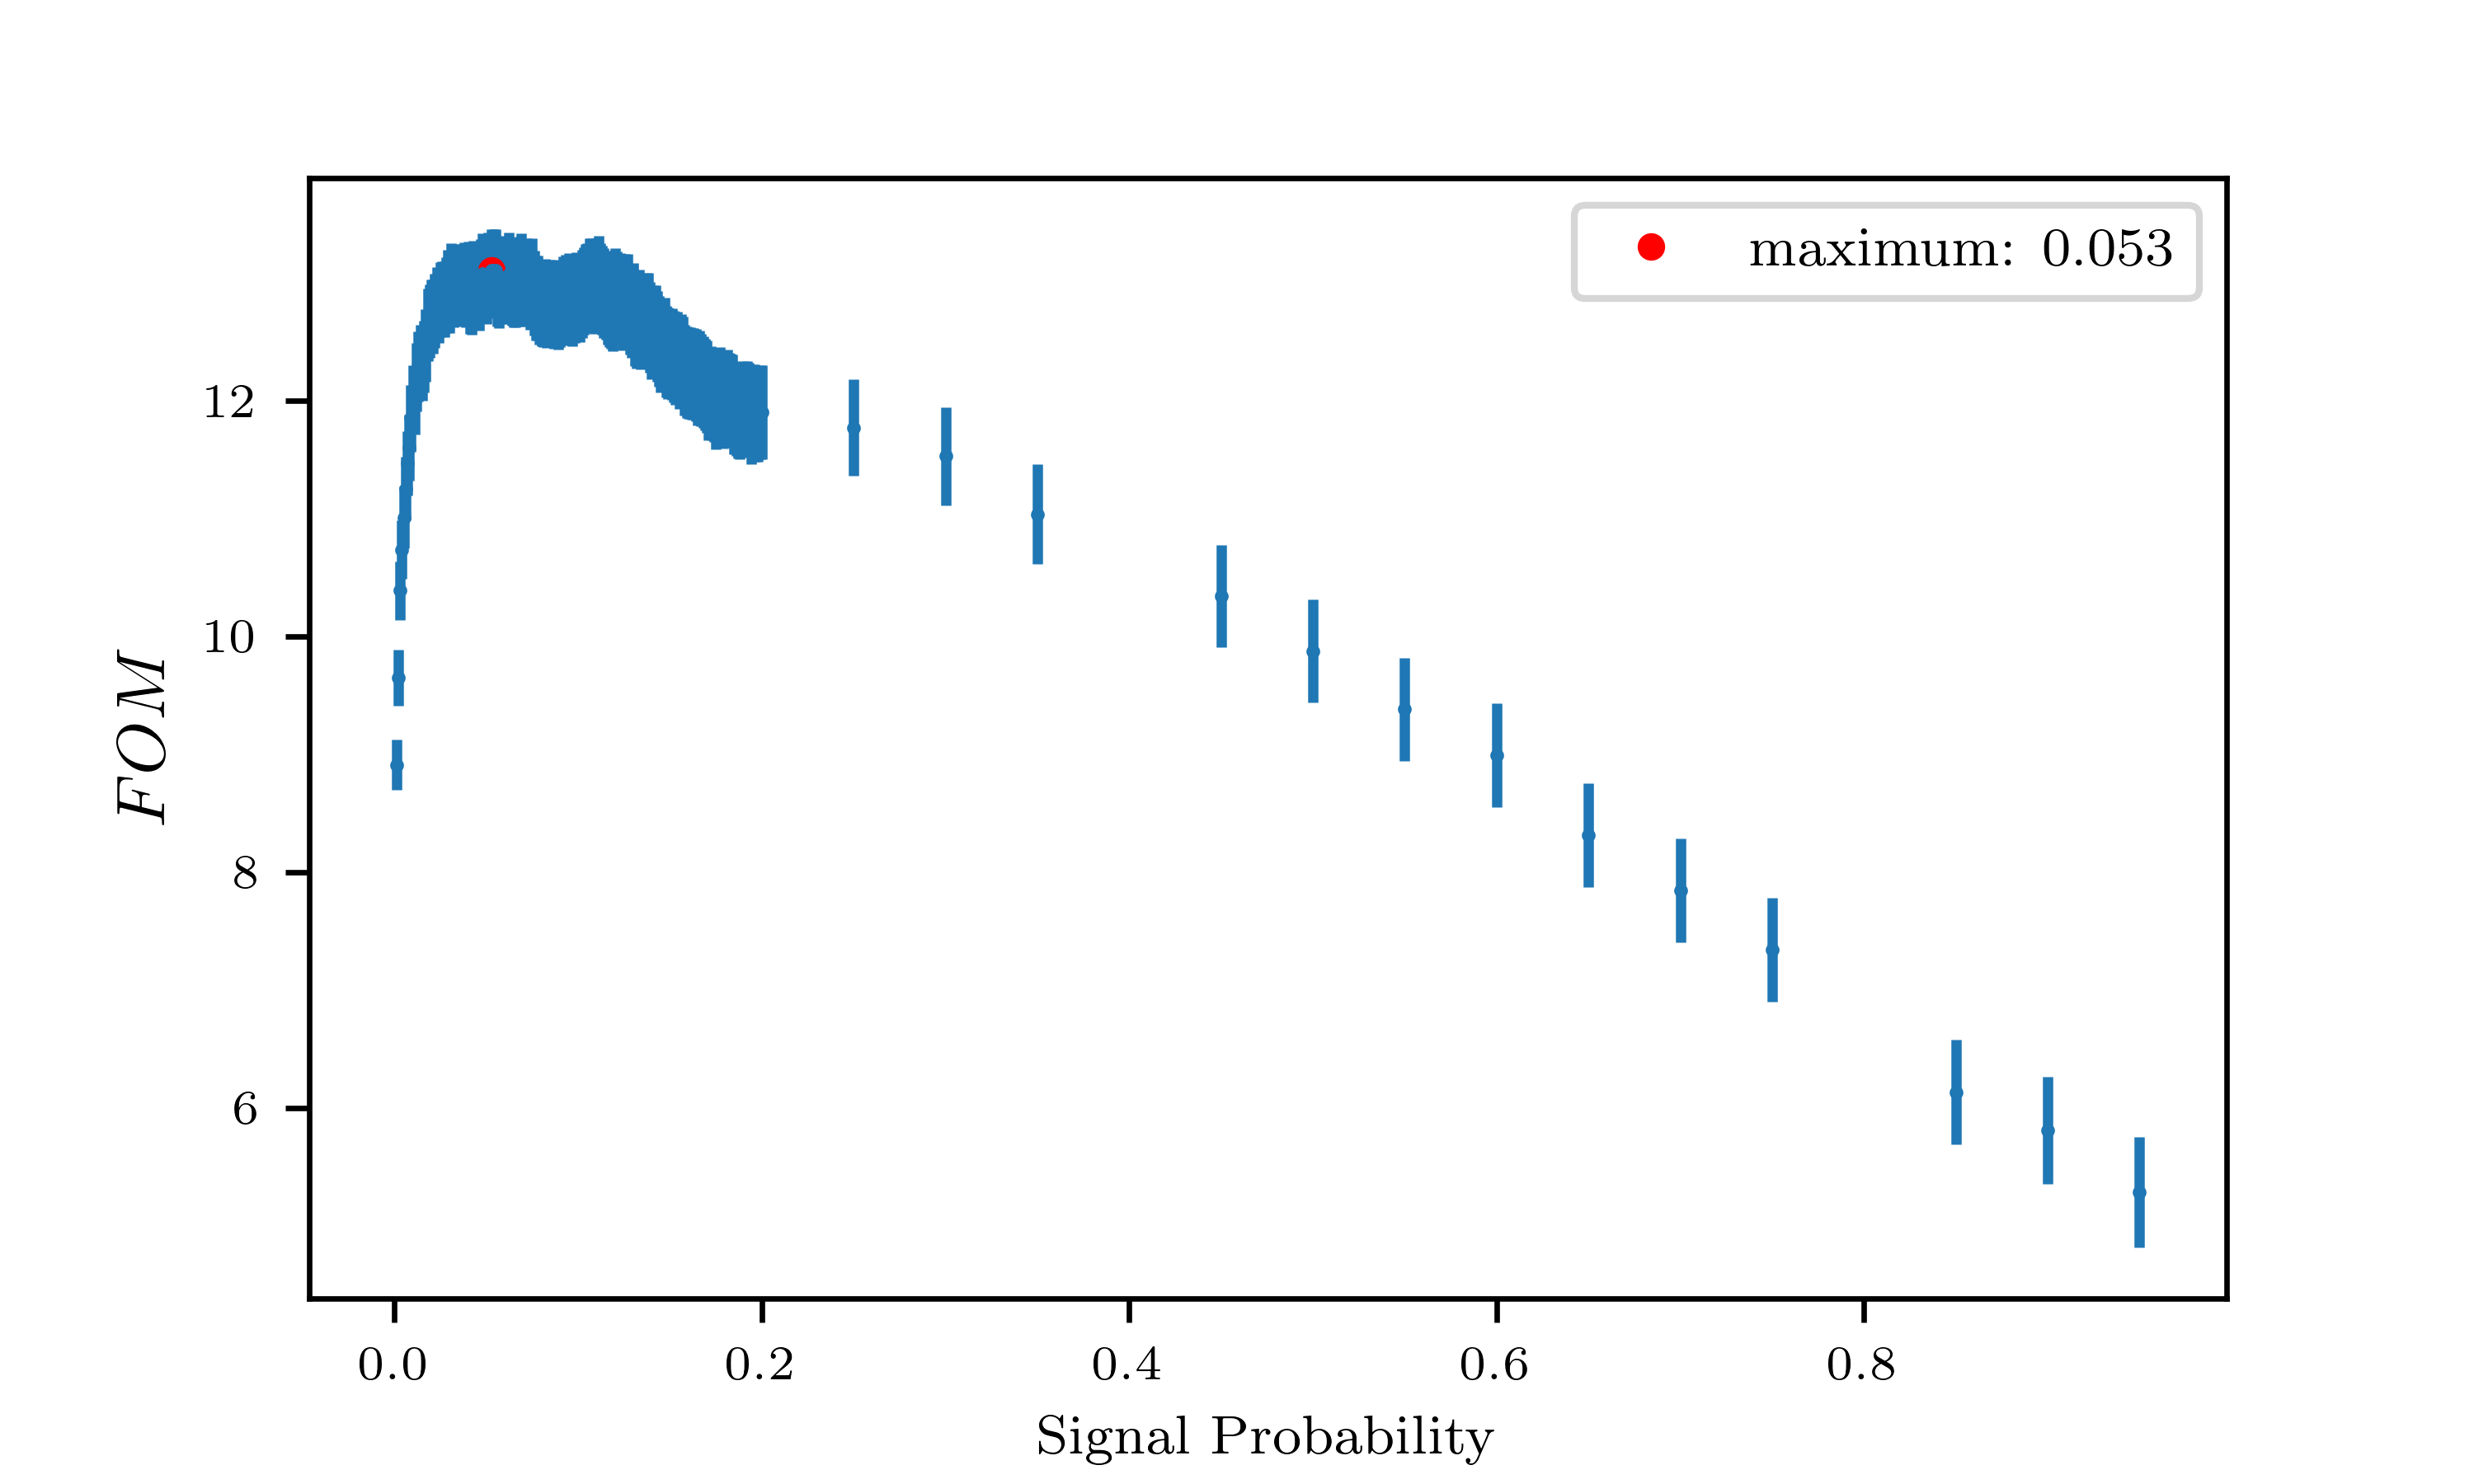
\includegraphics[width=0.75\textwidth]{03-Selection/figs/corr_B0_FOMvsSigProb_cut_until1.png}}
    \caption{Figure of Merit values calculated at several cuts on the SignalProbability variable}
    \label{fig:corr_B0_FOMvsSigProb_cut_until1}
    \end{figure}

\begin{figure}[H]
    %\centering
    {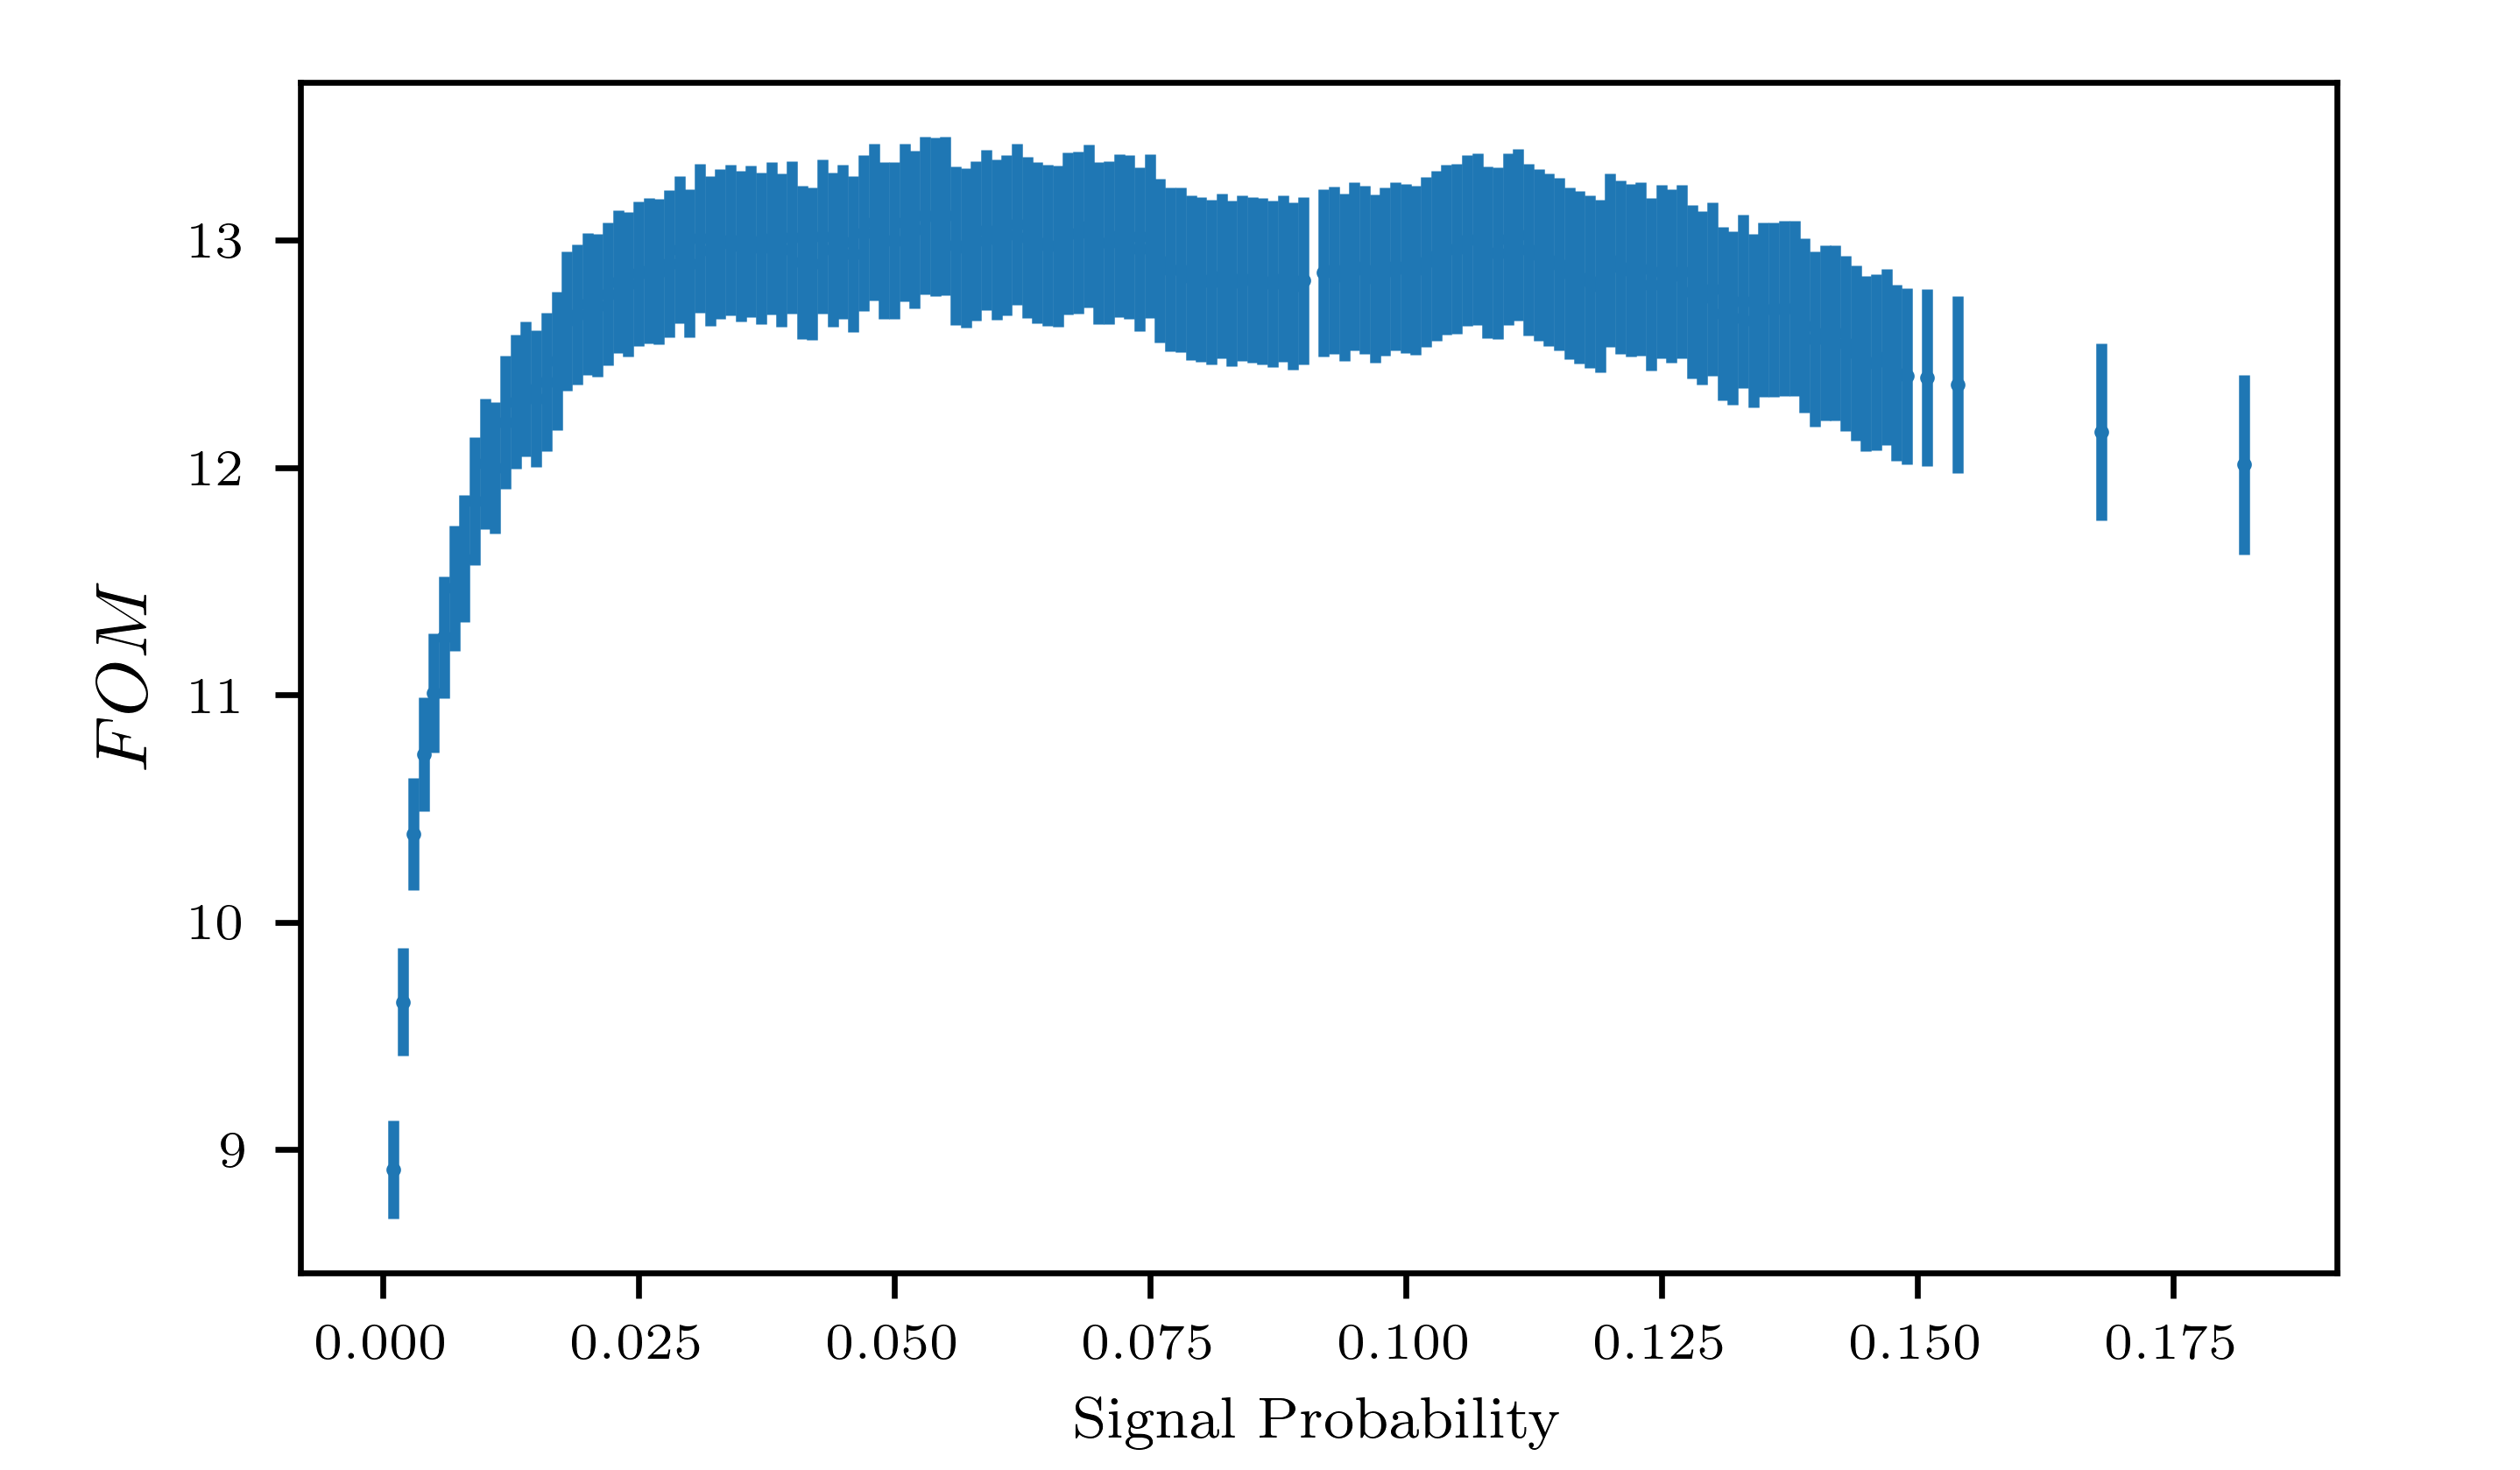
\includegraphics[width=0.75\textwidth]{03-Selection/figs/corr_B0_FOMvsSigProb_cut_until015.png}}
    \caption{Figure of Merit values calculated at several cuts on the SignalProbability variable}
    \label{fig:B0corrLambdaC_FOMvsSigProb}
    \end{figure}


The     $FOM$ curve for the $foxWolframR2$ variable is rechecked applying the chosen cut on SignalProbability
(\cref{fig:corr_B0SigProbOpt_FOMvsR2_cutRecheck}). As done in the other cases the final cut chosen is $foxWolframR2 < 0.3$ 
    \begin{figure}[H]
        %\centering
        {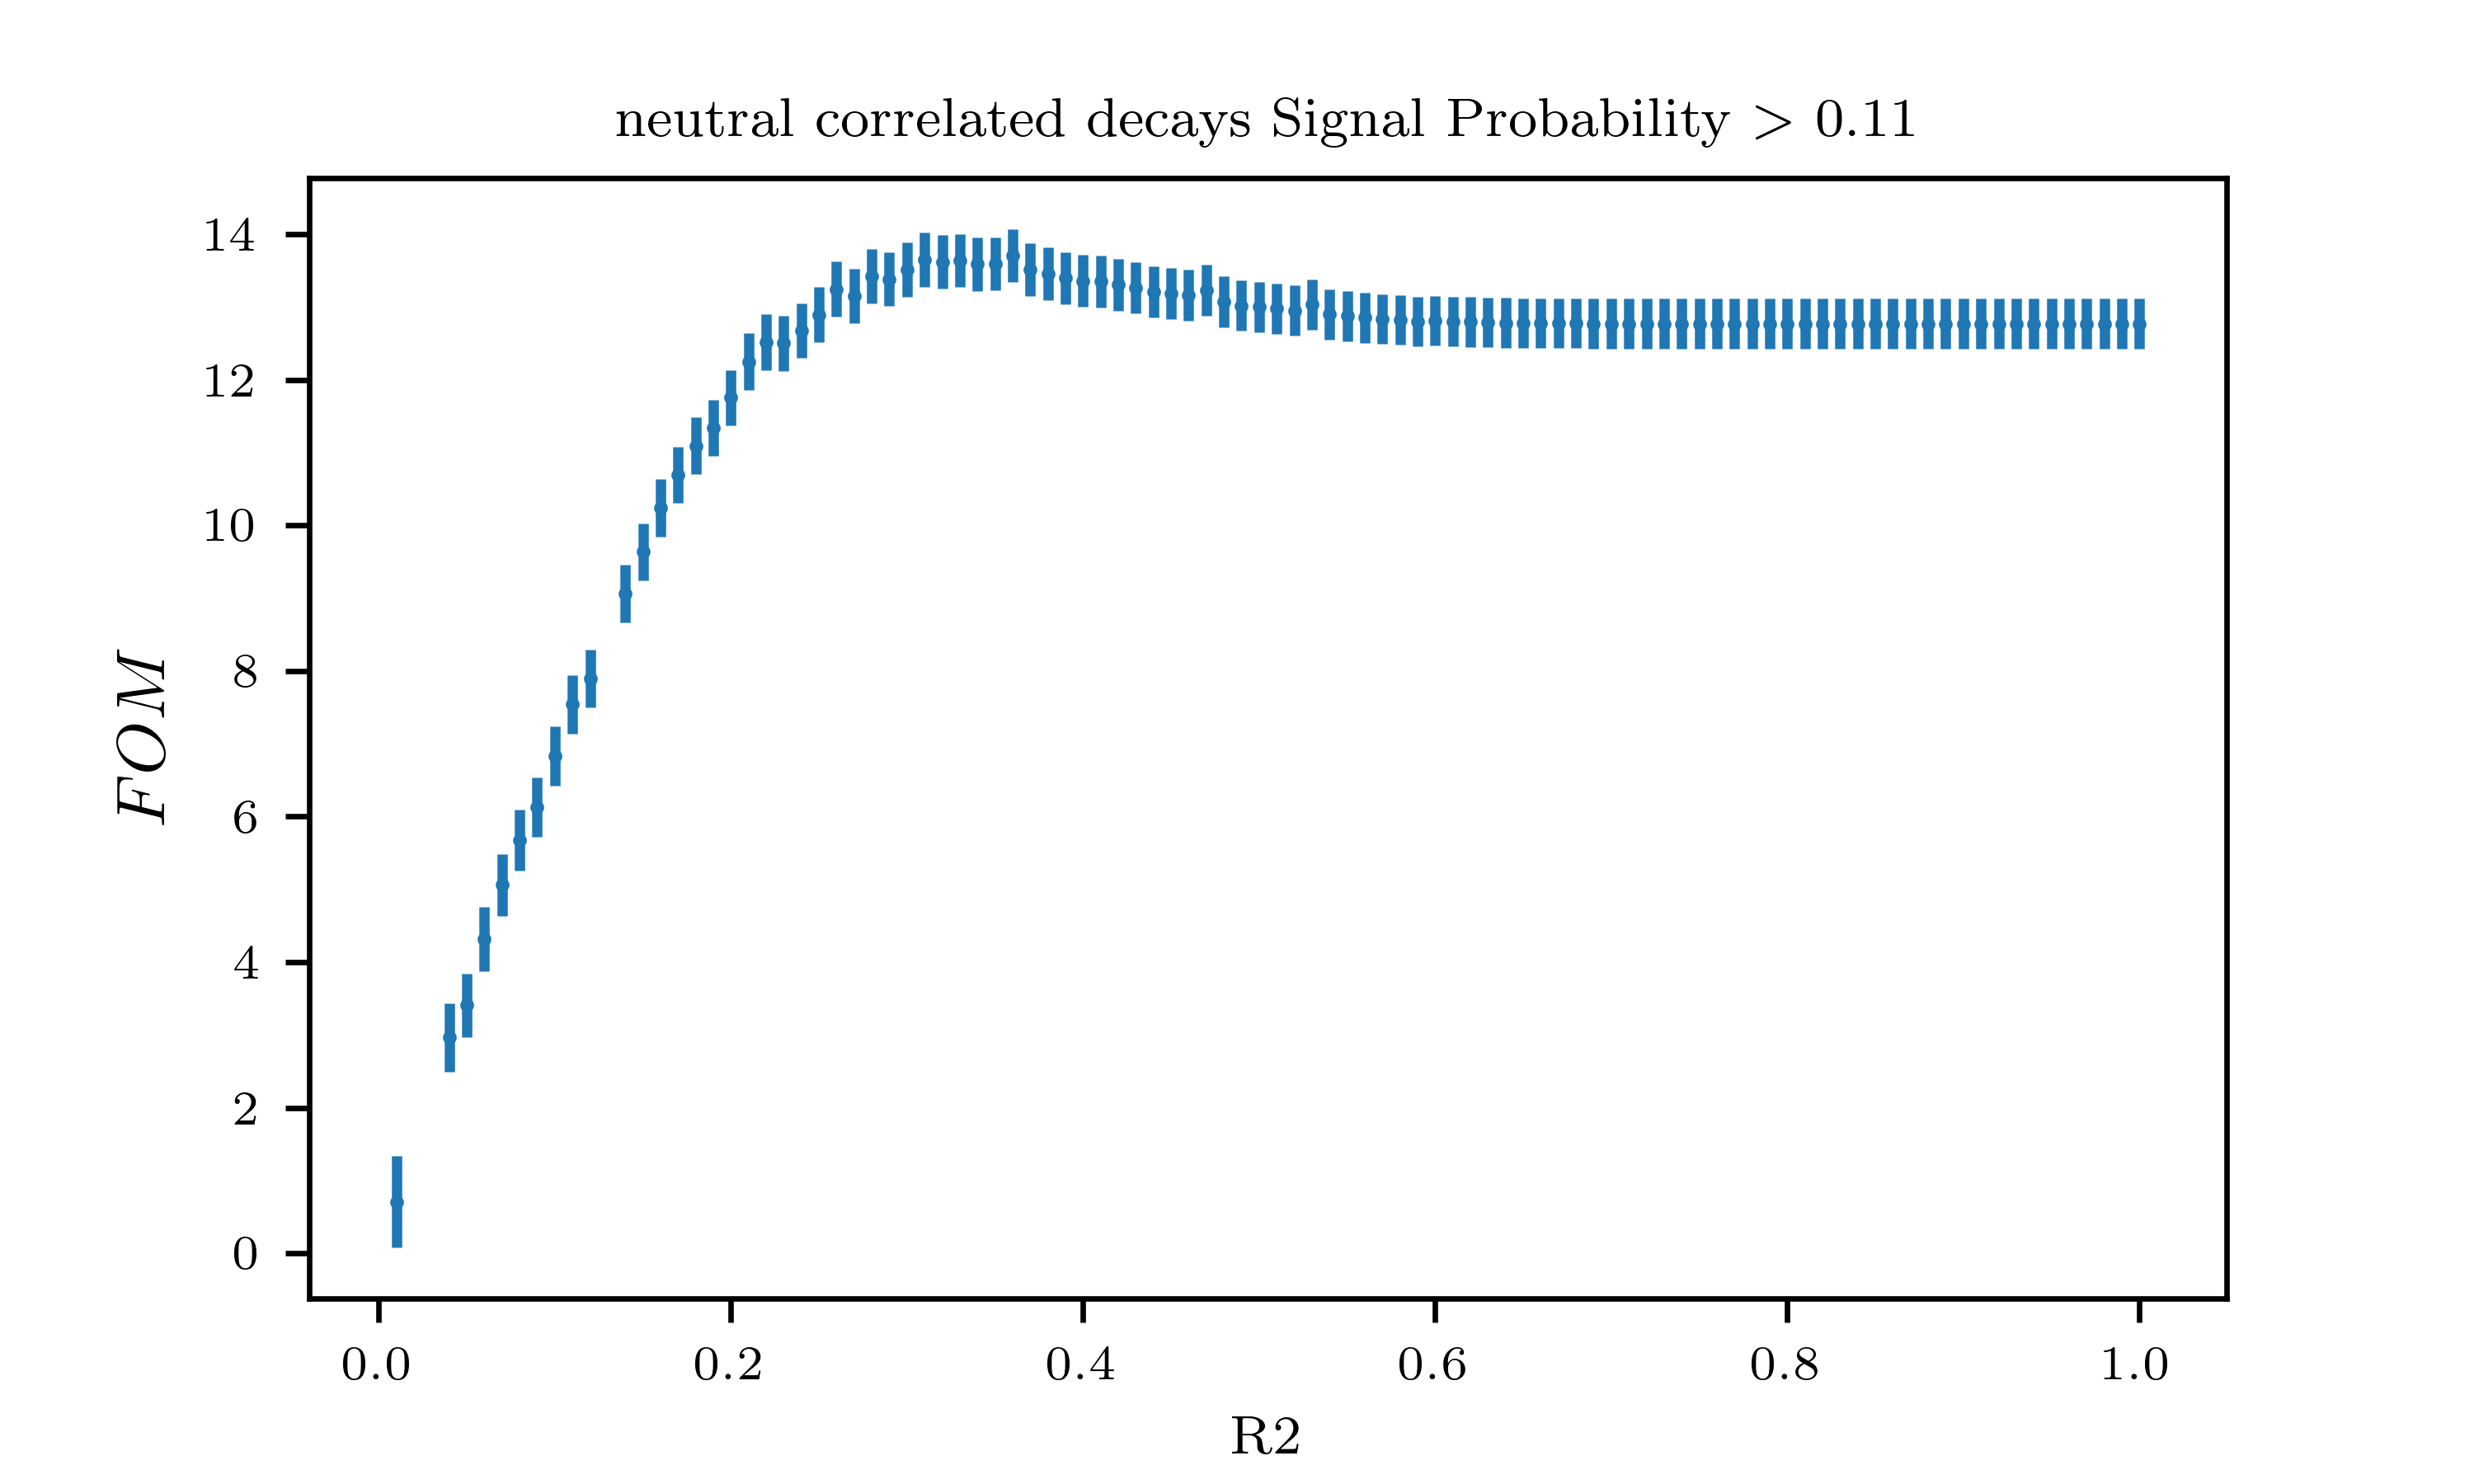
\includegraphics[width=0.75\textwidth]{03-Selection/figs/corr_B0SigProbOpt_FOMvsR2_cutRecheck.png}}
        \caption{Figure of Merit values calculated at several cuts on the $foxWolframR2$ variable}
        \label{fig:corr_B0SigProbOpt_FOMvsR2_cutRecheck}
        \end{figure}

    

 Using now the two optimized cuts to check the  $FOM$ curve for the momenta  a plateau appears for cuts starting from
 values around $p^{\Lambda_c}_{CMS} <$ 1.7 GeV/$c$ (see \cref{fig:corr_B0_FOMvsCMS_Pcut}).  In fact, around that value 
 the level of background becomes signifcantly higher compared to the amount o signal events as one can see in \cref{fig:B0corr_Lambda_c_CMS_P_optimisedSigProb_R}  


\begin{figure}[H]
    %\centering
    {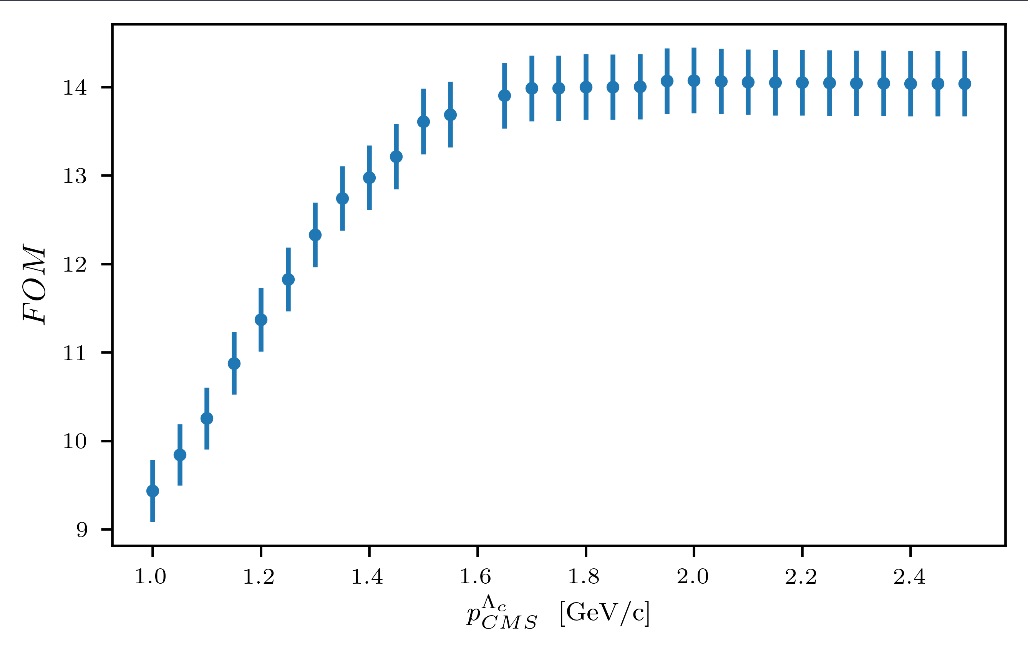
\includegraphics[width=0.85\textwidth]{03-Selection/figs/corr_B0_FOMvsCMS_Pcut.png}}
    \caption{Figure of Merit values calculated at several cuts on the momentum of the $\Lambda_c$ candidates in the center of mass system}
    \label{fig:corr_B0_FOMvsCMS_Pcut}
    \end{figure}



    \begin{figure}[H]
        %\centering
        {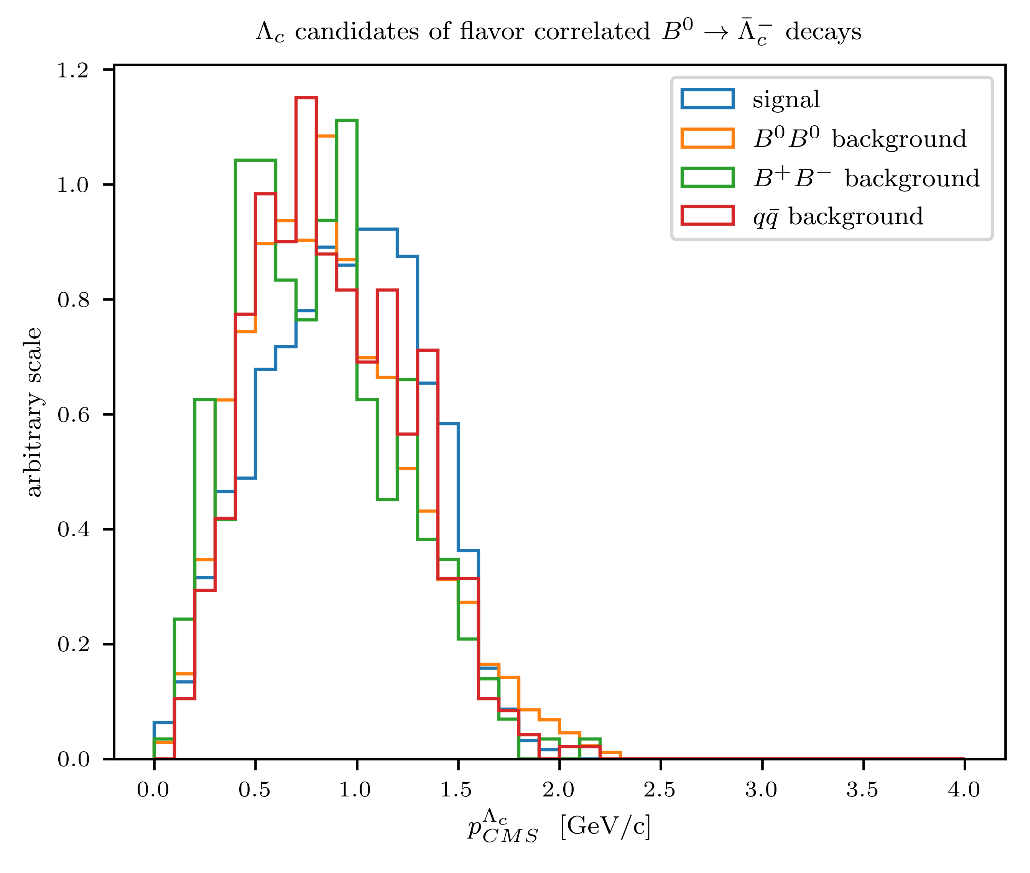
\includegraphics[width=0.85\textwidth]{03-Selection/figs/B0corr_Lambda_c_CMS_P_optimisedSigProb_R.png}}
        \caption{Distribution of  $\Lambda_c$ candidates momenta in the center of mass system}
        \label{fig:B0corr_Lambda_c_CMS_P_optimisedSigProb_R}
        \end{figure}
    

\cref{fig:B0corr_Mbc_MpKpi_optmised} shows the  $M_{bc} $ and $M(p K \pi)$ distributions after applying the following set of cuts:

\begin{itemize}
    \item $foxWolframR2  > $  0.3
    \item SignalProbability $>$ 0.11
    \item $p^{\Lambda_c}_{CMS} <$ 1.7 GeV/$c$
\end{itemize}
 

\begin{figure}[H]
%\centering
{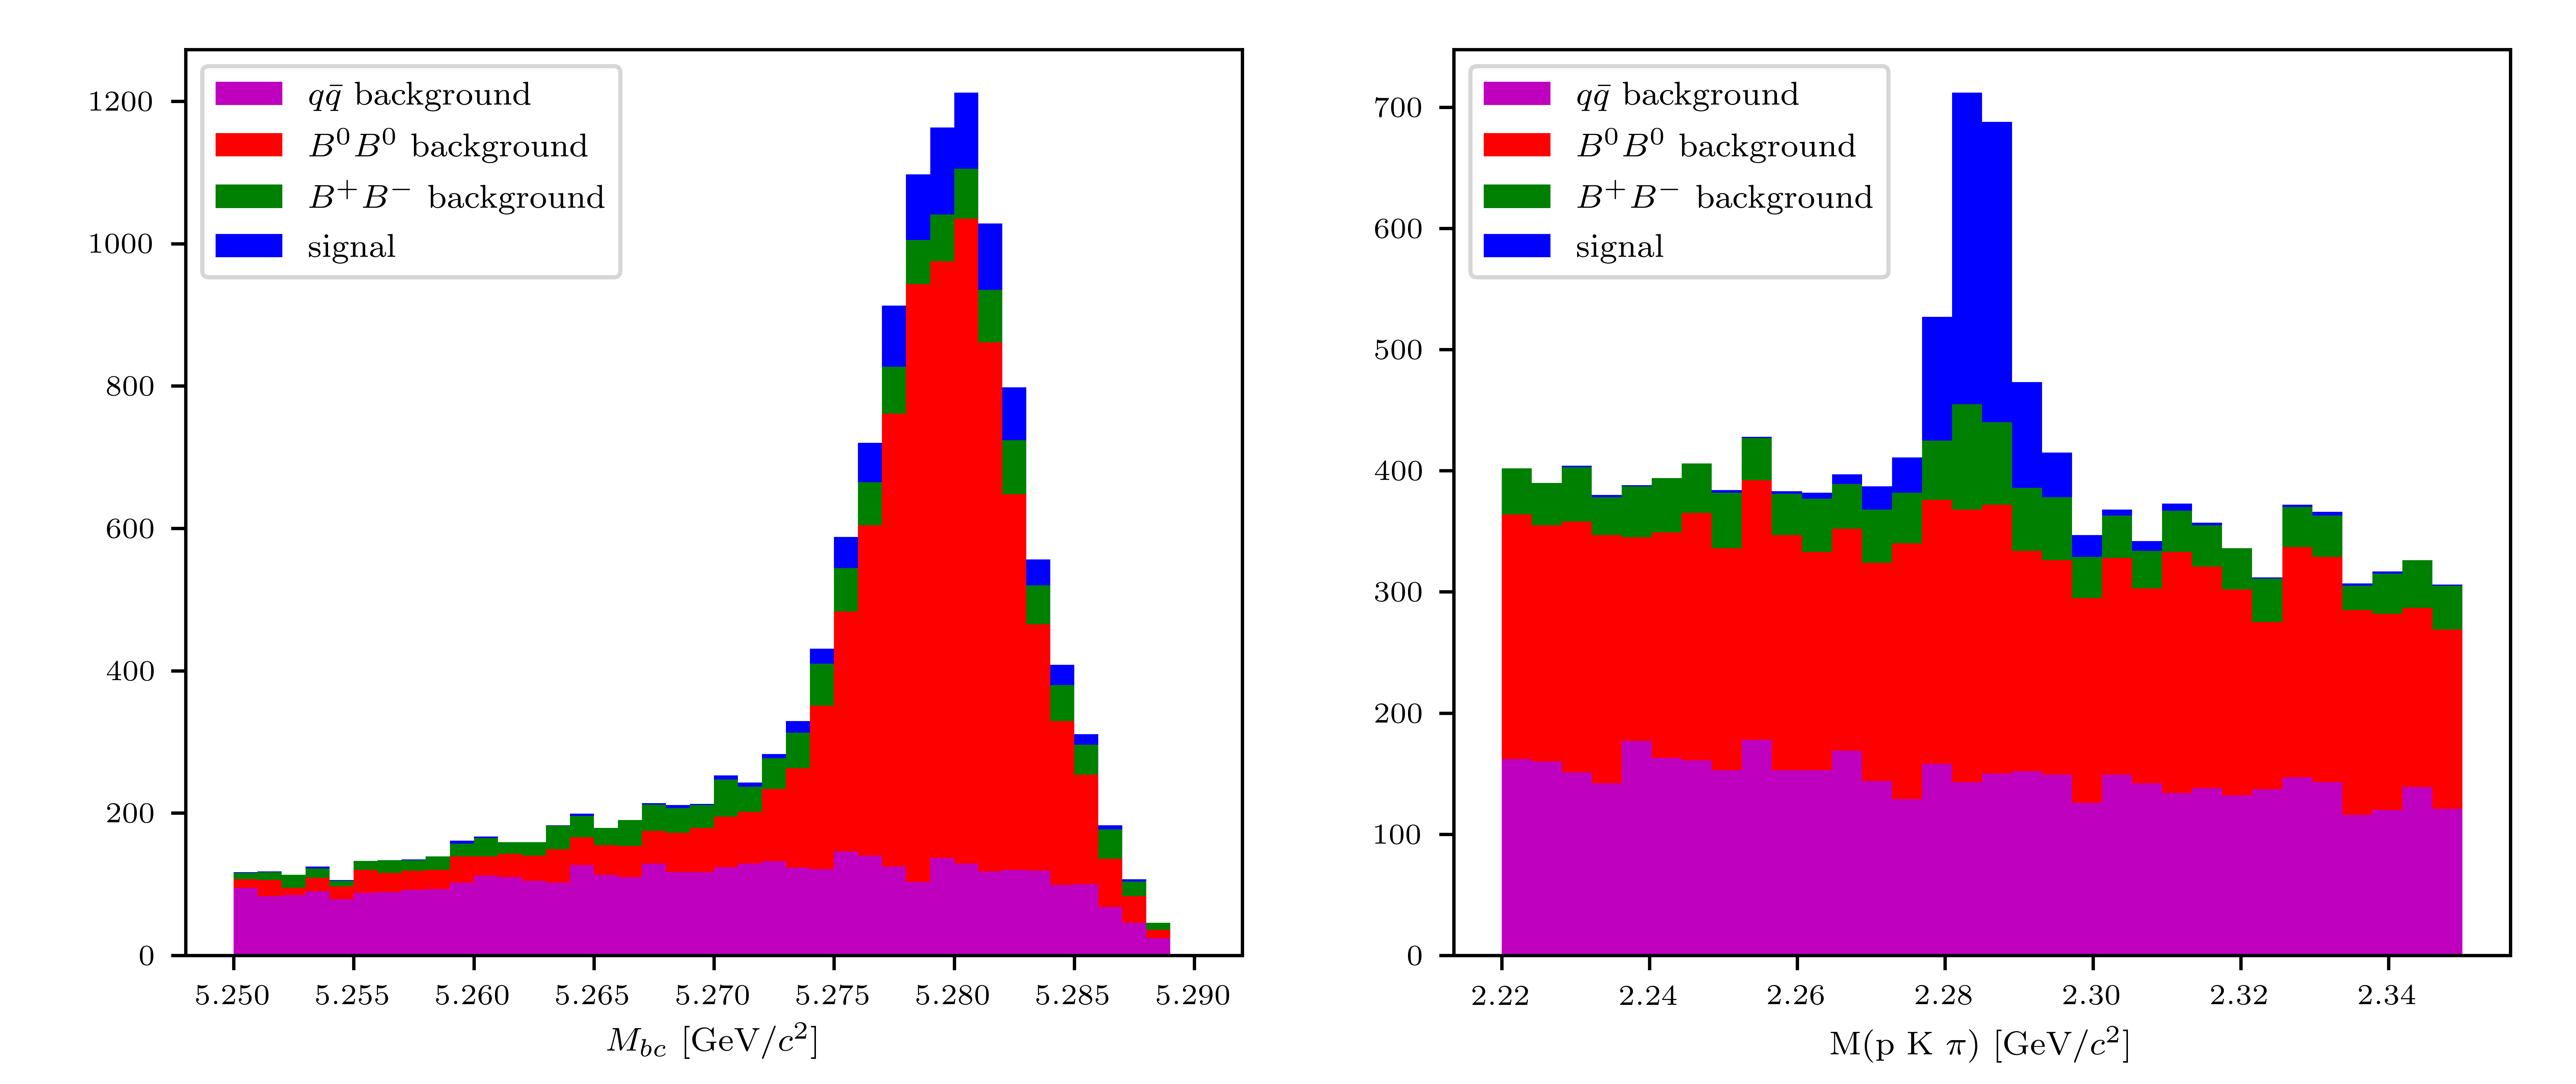
\includegraphics[width=0.95\textwidth]{03-Selection/figs/B0corr_Mbc_MpKpi_optmised.png}}
\caption{Distribution of $M_{bc} $ (left) and invariant mass of neutral correlated $\Lambda_c$  candidates (right), in the signal region after the above mentioned selection cuts.}
\label{fig:B0corr_Mbc_MpKpi_optmised}
\end{figure}



                               
\subsection{$B^0 \rightarrow \Lambda_c^+$ decays}
\label{sec:neutralAcorrBtoLambdaC}


Finally same procedure is applied also to the neutral anticorrelated decays. 
The final selections for the variables of  $foxWolframR2 $,  SignalProbability and the momentum of the $\Lambda_c$ candidates in the center of mass system:


\begin{itemize}
    \item $foxWolframR2  < $  0.3
    \item SignalProbability $>$ 0.15
    \item $p^{\Lambda_c}_{CMS} <$ 1.4 GeV/$c$
\end{itemize}    

\cref{fig:B0acorr_Mbc_MpKpi_optmised} shows the  $M_{bc} $ and $M(p K \pi)$ distributions after applying these cuts.
\begin{figure}[h!]
    %\centering
    {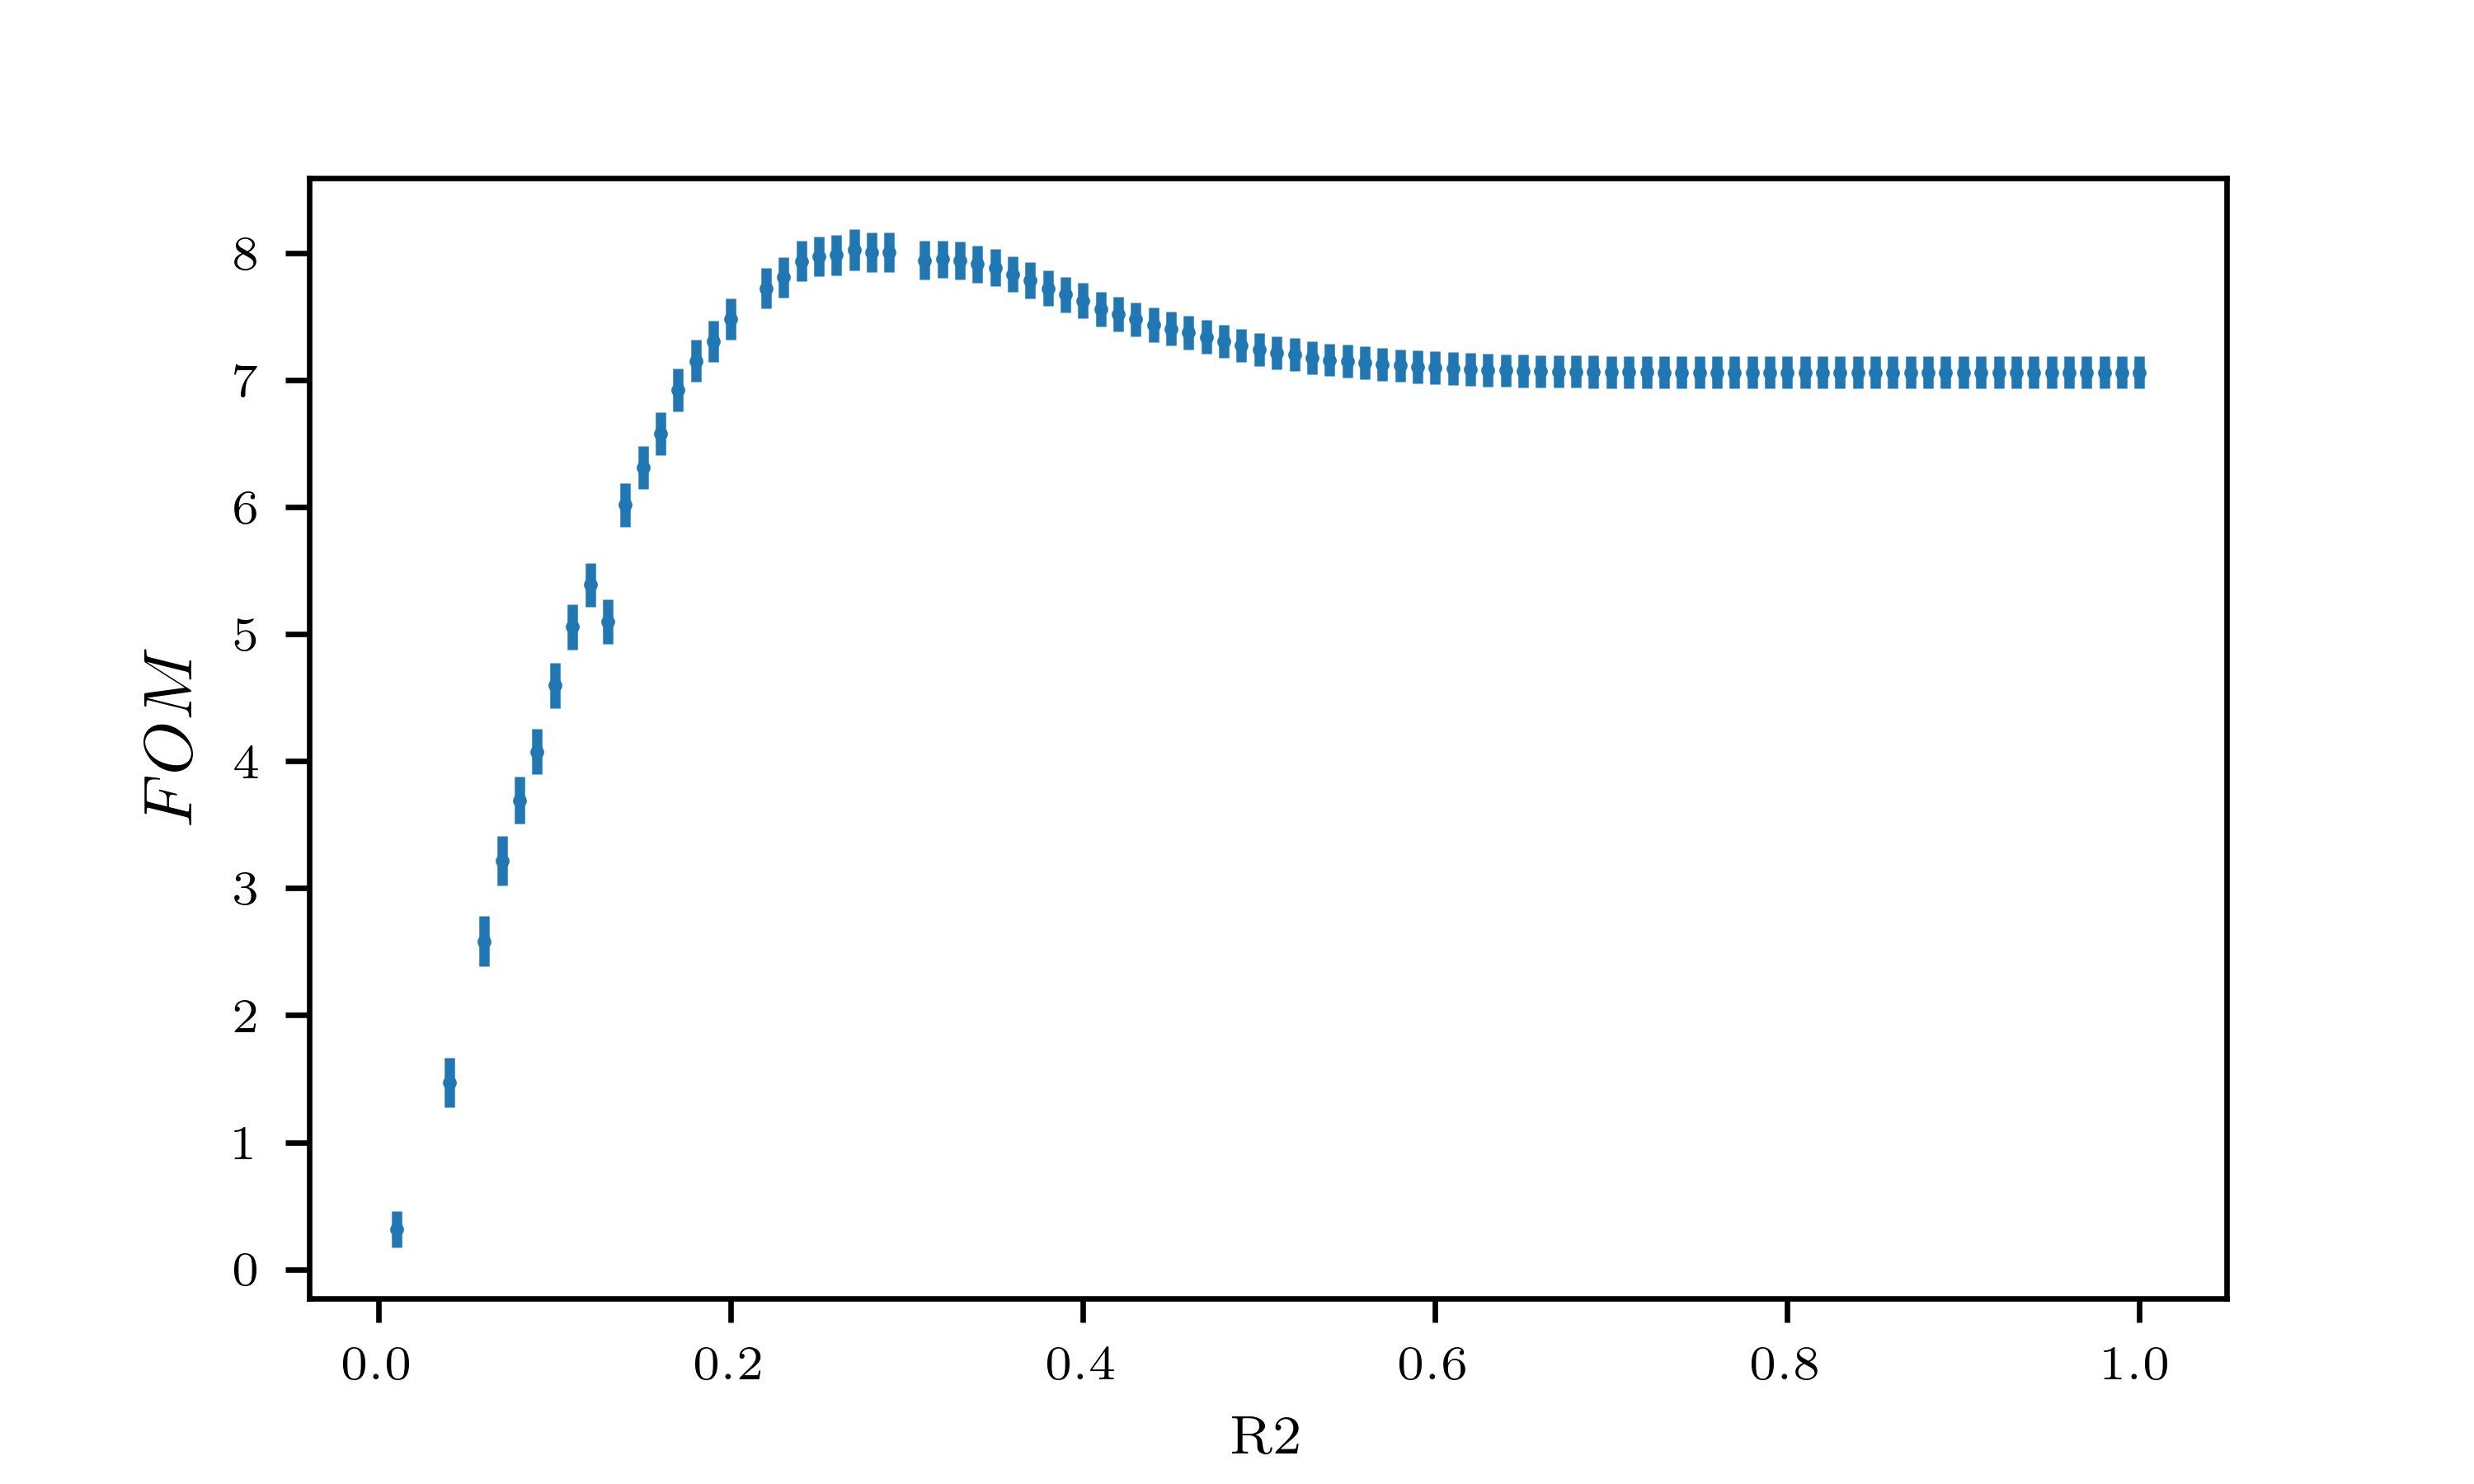
\includegraphics[width=0.75\textwidth]{03-Selection/figs/acorr_chargedB_FOMvsR2_cut.png}}
    \caption{Figure of Merit values calculated at several cuts on the $foxWolframR2$ variable}
    \label{fig:acorr_chargedB_FOMvsR2_cut}
    \end{figure}



\begin{figure}[h!]
    %\centering
    {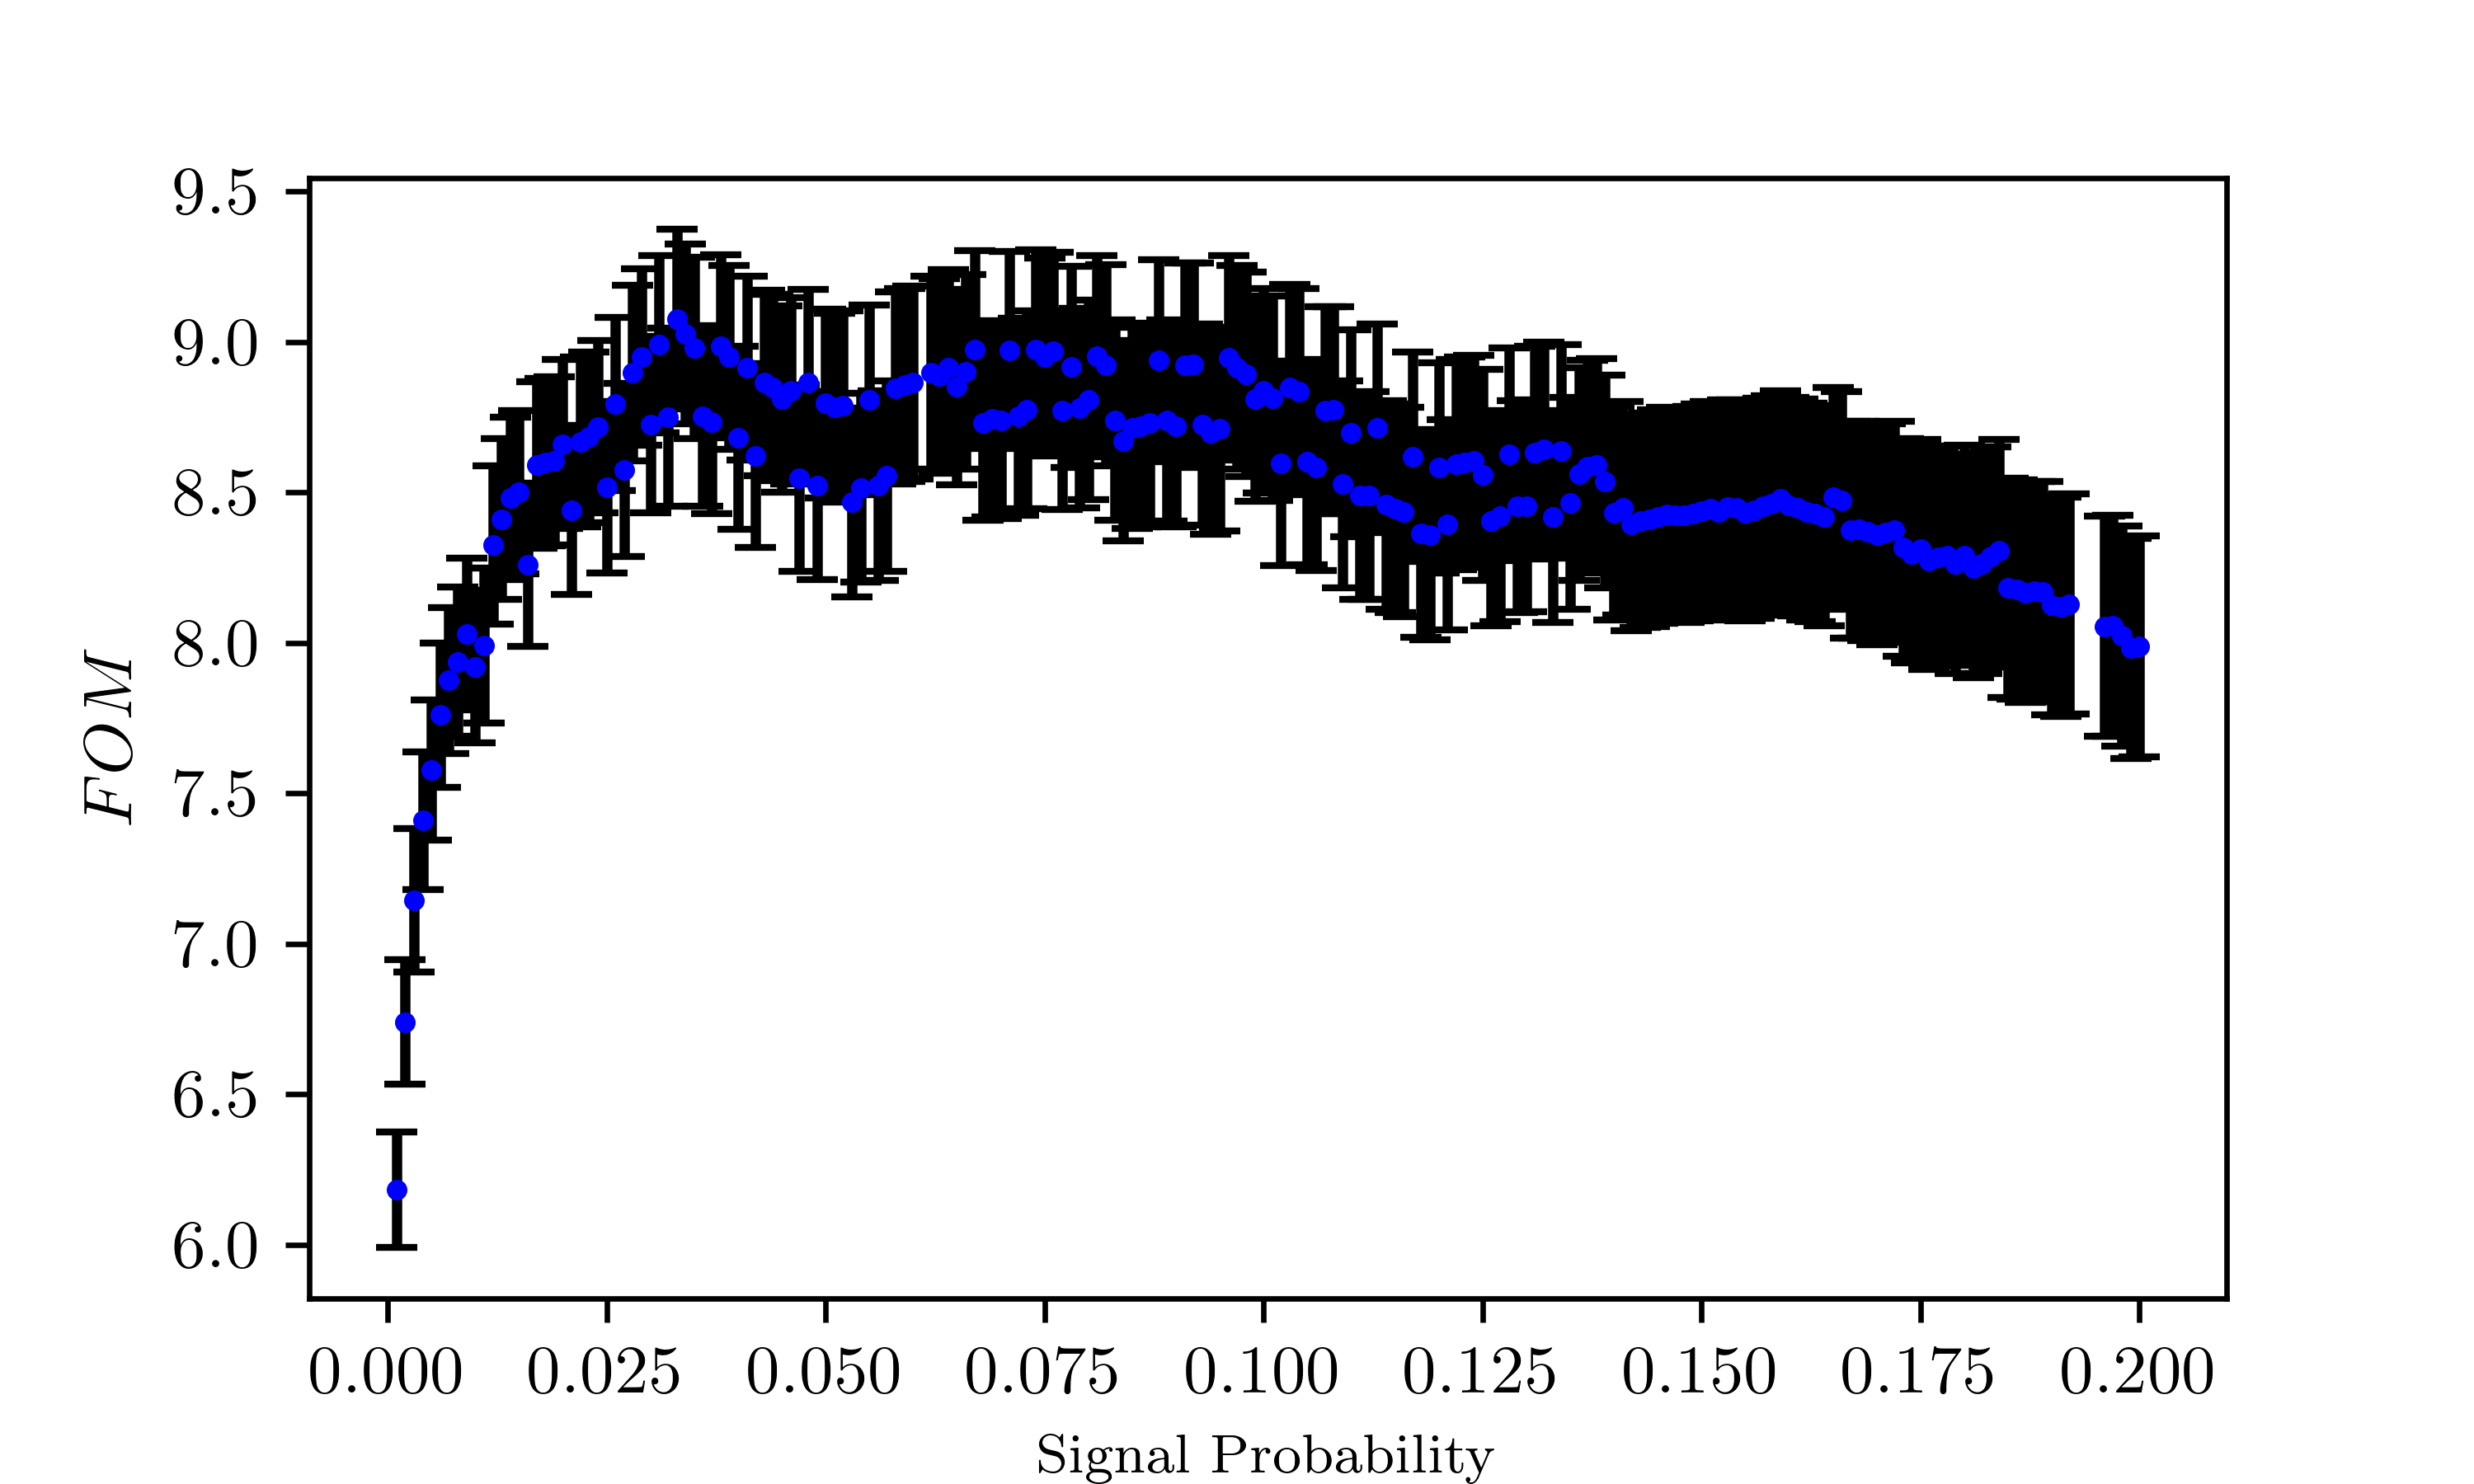
\includegraphics[width=0.85\textwidth]{03-Selection/figs/acorr_B0_FOMvsSigProb_cut.png}}
    \caption{Figure of Merit values calculated at several cuts on the SignalProbability variable}
    \label{fig:acorr_neutralB_FOMvsR2_cut}
    \end{figure}

\newpage

\begin{figure}[h!]
        %\centering
        {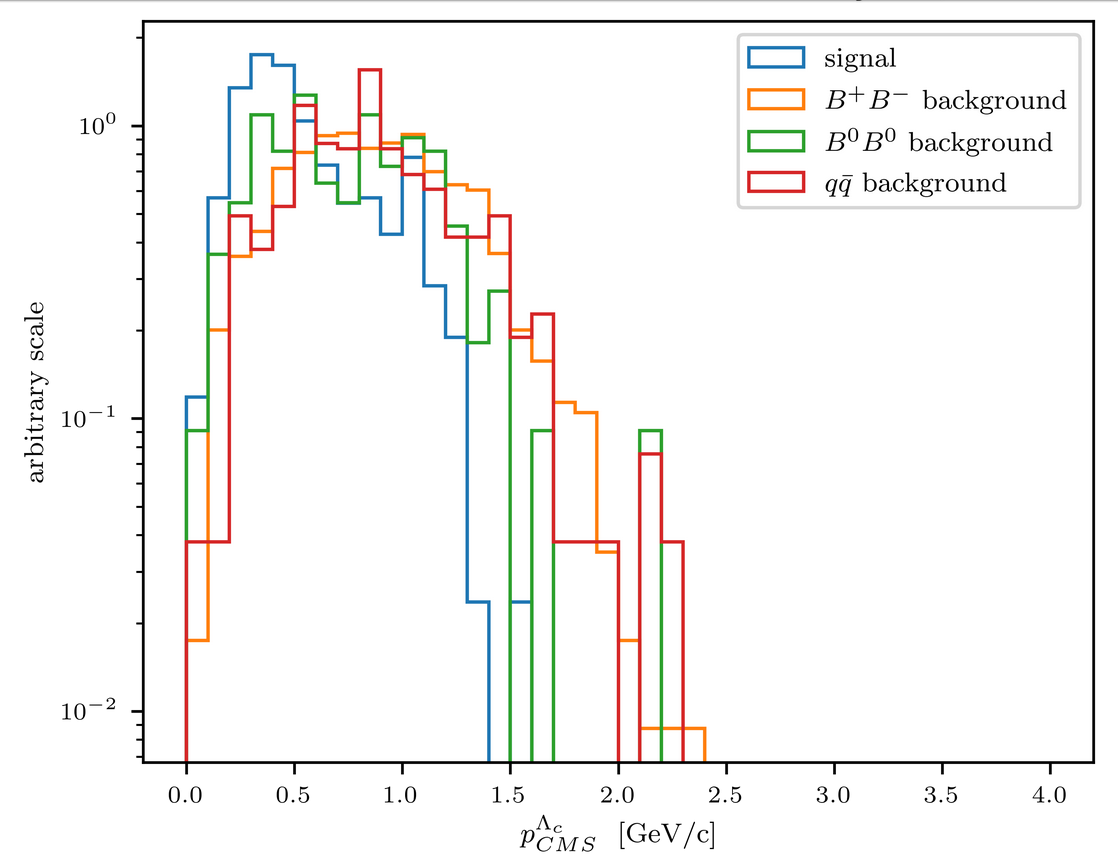
\includegraphics[width=0.75\textwidth]{03-Selection/figs/acorrB0_Lambda_c_CMS_P_optimisedSigProb_R.png}}
        \caption{Distribution of  $\Lambda_c$ candidates momenta in the center of mass system}
        \label{fig:acorrB0_Lambda_c_CMS_P_optimisedSigProb_R}
        \end{figure}

    \begin{figure}[h!]
        %\centering
        {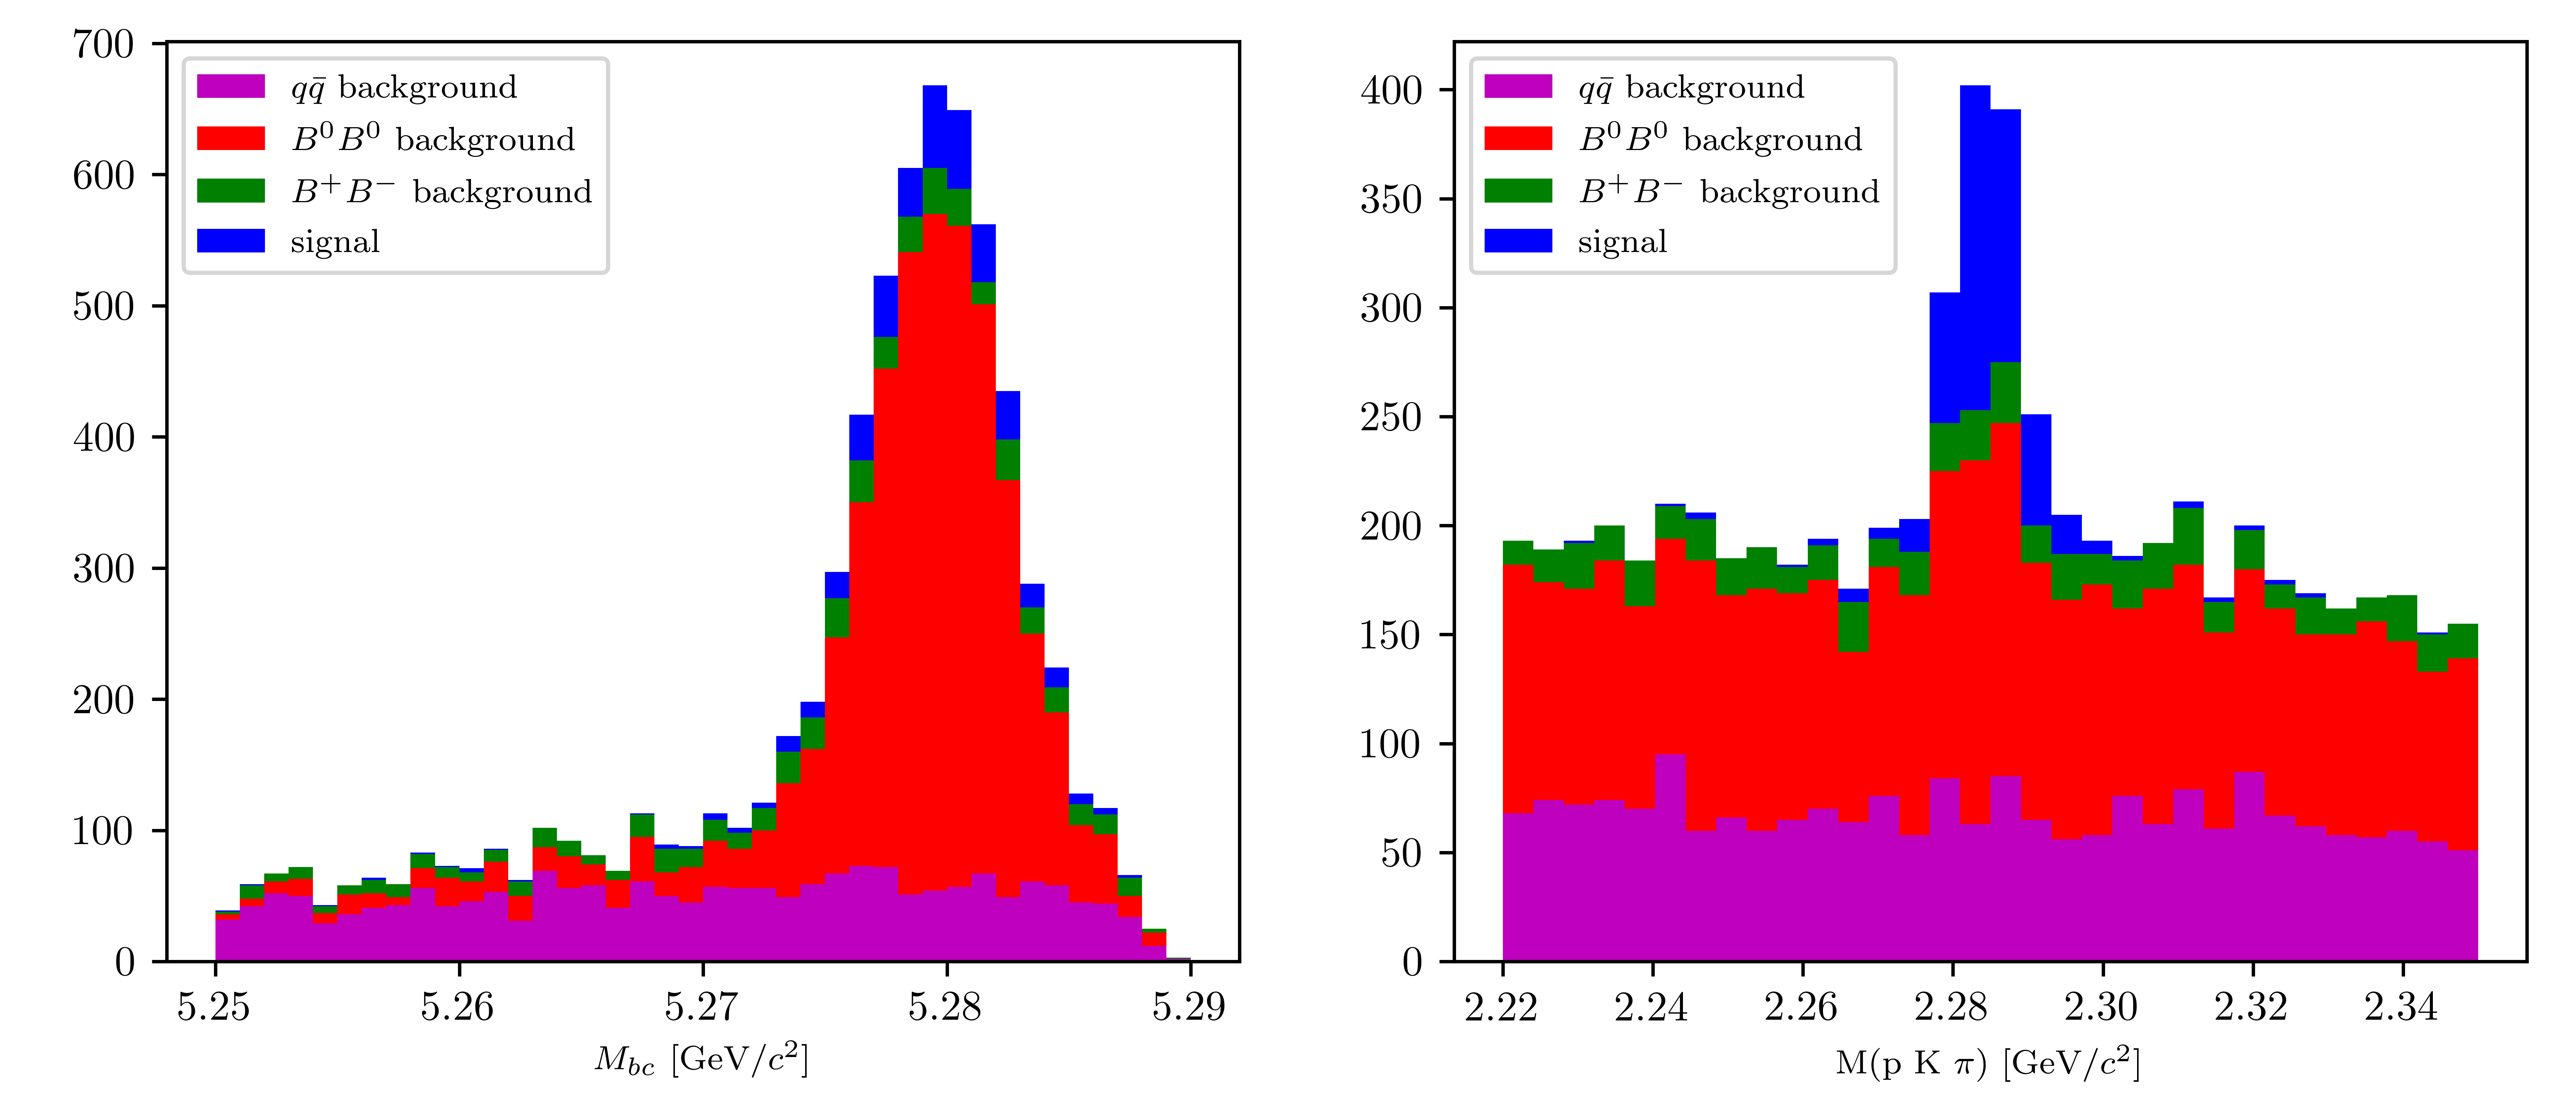
\includegraphics[width=0.95\textwidth]{03-Selection/figs/B0acorr_Mbc_MpKpi_optmised.png}}
        \caption{Distribution of $M_{bc} $ (left) and invariant mass of neutral anticorrelated $\Lambda_c$  candidates (right), in the signal region after the above mentioned selection cuts.}
        \label{fig:B0acorr_Mbc_MpKpi_optmised}
        \end{figure}
                            

        \newpage